\documentclass[11pt,a4paper]{report}
% ==========================
%     ENCODAGE & LANGUE
% ==========================
\usepackage[utf8]{inputenc}
\usepackage[T1]{fontenc}
\usepackage[french]{babel}
\usepackage{setspace}
\usepackage{csquotes}
\usepackage{siunitx}

% ==========================
%     MISE EN PAGE
% ==========================
\usepackage[a4paper,top=2.4cm,bottom=2.6cm,inner=2.6cm,outer=2.2cm]{geometry}
\usepackage[dvipsnames]{xcolor}
\usepackage{fancyhdr}
\definecolor{ReportBlue}{HTML}{1F4E79}
\definecolor{ReportDark}{HTML}{1F2933}
\definecolor{ReportGray}{HTML}{5C6670}
\definecolor{ReportLink}{HTML}{0B5CAD}
\setlength\headheight{16pt}
\emergencystretch=2em
\pagestyle{fancy}
\fancyhf{}
\fancyhead[L]{\small\textcolor{ReportGray}{Rapport M2 -- SDHCAL}}
\fancyhead[R]{\small\nouppercase{\leftmark}}
\fancyfoot[C]{\small\thepage}
\renewcommand{\headrulewidth}{0.4pt}
\renewcommand{\footrulewidth}{0pt}
\fancypagestyle{plain}{
  \fancyhf{}
  \fancyfoot[C]{\small\thepage}
  \renewcommand{\headrulewidth}{0pt}
}

% ==========================
%     POLICE & MICROTYPE
% ==========================
\usepackage{fourier}
\usepackage[protrusion=true,expansion=true]{microtype}

% ==========================
%     FIGURES & TABLEAUX
% ==========================
\usepackage{graphicx}
\usepackage{subcaption}
\usepackage{booktabs}
\usepackage{tabularx}
\usepackage[font=small,labelfont={bf,color=ReportBlue},labelsep=period]{caption}
\usepackage{float}
\usepackage{wrapfig}
\usepackage{tikz}
% ==========================
%     MATHS & LISTES
% ==========================
\usepackage{amsmath,amssymb}
\usepackage{enumitem}
\setlist{topsep=0.35em,itemsep=0.2em,parsep=0.1em}

% ==========================
%     LIENS
% ==========================
\usepackage[colorlinks=true,linkcolor=ReportBlue,citecolor=ReportBlue,urlcolor=ReportLink]{hyperref}
\usepackage{bookmark}
\hypersetup{
  pdftitle={Rapport de stage M2 -- PID et reconstruction d'energie dans le SDHCAL},
  pdfauthor={Mohamed Yanis IDIR},
  pdfsubject={Rapport de stage de Master 2},
  pdfkeywords={SDHCAL, calorimetrie hadronique, identification des particules, apprentissage automatique}
}

% ==========================
%     BIBLIOGRAPHIE (optionnelle)
% ==========================
\usepackage[backend=biber,sorting=none]{biblatex}
\addbibresource{references.bib}

% ==========================
%     TITRES
% ==========================
\usepackage{titlesec}
\titleformat{\chapter}[display]
  {\normalfont\huge\bfseries\color{ReportBlue}}
  {\chaptertitlename\ \thechapter}
  {0.35em}
  {\Huge\color{ReportDark}}
  [\vspace{0.4ex}\titlerule]
\titleformat{name=\chapter,numberless}[display]
  {\normalfont\huge\bfseries\color{ReportBlue}}
  {}
  {0pt}
  {\Huge\color{ReportDark}}
  [\vspace{0.4ex}\titlerule]
\titlespacing*{\chapter}{0pt}{-0.5cm}{1.2cm}
\titleformat{\section}
  {\Large\bfseries\color{ReportBlue}}
  {\thesection}
  {0.8em}
  {}
\titleformat{\subsection}
  {\large\bfseries\color{ReportDark}}
  {\thesubsection}
  {0.8em}
  {}
\titleformat{\subsubsection}{\large\bfseries}{\thesubsubsection}{1em}{}

% ==========================
%     COMMANDES UTILES
% ==========================
\newcommand{\HRule}[1]{\textcolor{ReportBlue}{\rule{\linewidth}{#1}}}
\newcommand{\code}[1]{\texttt{#1}}
\newcommand{\E}[1]{\times 10^{#1}}

% ==========================
%     PROFONDEUR TOC
% ==========================
\onehalfspacing
\setcounter{tocdepth}{2}
\setcounter{secnumdepth}{2}
\makeatletter
\renewcommand{\@pnumwidth}{2.2em}
\renewcommand{\@tocrmarg}{3.0em}
\makeatother

% ==========================
%     DOCUMENT
% ==========================
\begin{document}
\date{}
\hypersetup{pageanchor=false}
\pagenumbering{gobble}

% ==========================
%     PAGE DE GARDE
% ==========================
\begin{titlepage}
  \thispagestyle{empty}

  % Logos
  \begin{minipage}[c]{0.45\textwidth}
    \centering
    
\includegraphics[width=38mm]{img/ucbl_logo.png}\\[0.25cm]
    {\small Université Claude Bernard Lyon 1}
  \end{minipage}\hfill
  \begin{minipage}[c]{0.45\textwidth}
    \centering
    
\includegraphics[width=46mm]{img/Logo_IP2I.png}\\[0.25cm]
    {\small Institut de Physique des Deux Infinis de Lyon (IP2I)}
  \end{minipage}

  \vspace{3cm}
  \begin{center}
    \HRule{1.2pt}\vspace{0.6cm}

    {\LARGE\bfseries
      Identification des particules hadroniques et reconstruction de l’énergie\\
      dans un calorimètre SDHCAL à l’aide de méthodes d’apprentissage automatique
    \par}

    \vspace{0.6cm}
    \HRule{1.2pt}

    \vspace{0.8cm}
    {\large \textsc{Rapport de stage}}\\[0.3cm]
    {\normalsize Année universitaire 2024--2025}
  \end{center}

  \vfill

  \begin{center}
    {\normalsize
      Mohamed Yanis IDIR \\[0.2cm]
      Master Physique Subatomique
    }\par
    \vspace{0.6cm}
    {\normalsize \textbf{Encadré par :}}\\[0.1cm]
    {\normalsize
      Pr.~Imad Laktineh, Université Lyon~1 \\[-1pt]
      Pr.~Gérald Grenier, Université Lyon~1
    }
  \end{center}
\end{titlepage}
\clearpage
\hypersetup{pageanchor=true}
\pagenumbering{roman}

% ==========================
%     TABLE DES MATIÈRES
% ==========================
\newpage
\tableofcontents
\newpage

% ==========================
%     RÉSUMÉ
% ==========================
\chapter*{Résumé}
\phantomsection
\addcontentsline{toc}{chapter}{Résumé}

La mesure précise de l’énergie des hadrons constitue un enjeu majeur de la physique des hautes énergies. Contrairement aux gerbes électromagnétiques, relativement stables et bien modélisées, les gerbes hadroniques présentent d’importantes fluctuations événement par événement, liées notamment à la fraction électromagnétique, aux pertes d’énergie invisibles ainsi qu’aux fuites longitudinales et latérales. Ces effets dégradent la linéarité de la réponse calorimétrique et limitent la résolution en énergie.

Le \emph{Semi-Digital Hadron CALorimeter} (SDHCAL) propose une approche originale fondée sur une très haute granularité spatiale associée à une lecture semi-digitale à trois seuils. Une telle architecture permet d’accéder finement à la topologie des gerbes hadroniques et ouvre des perspectives intéressantes aussi bien pour l’identification des particules que pour la reconstruction de leur énergie.

Dans ce travail, une chaîne d’analyse complète a été développée et appliquée à des échantillons simulés de pions, protons et kaons neutres longs. L’identification hadronique repose principalement sur des arbres de décision boostés (\emph{Boosted Decision Trees}, BDT), tandis qu’une étude exploratoire de réseaux de neurones graphiques (GNN) a également été menée. Pour la reconstruction de l’énergie, deux approches ont été comparées : une méthode paramétrique fondée sur un ajustement par minimisation du $\chi^2$ des compteurs multi-seuils, et une régression supervisée par BDT exploitant un ensemble enrichi de descripteurs de gerbe.

Les performances ont ensuite été étudiées dans plusieurs scénarios réalistes combinant identification des particules et reconstruction d’énergie, afin de quantifier l’apport du PID sur la calibration calorimétrique.

Les résultats montrent que l’identification préalable des particules améliore la linéarité de la réponse et réduit les biais de reconstruction. Ils confirment également que les méthodes modernes d’apprentissage automatique constituent une voie prometteuse pour exploiter pleinement le potentiel des calorimètres hadroniques hautement granulaires dans les futurs collisionneurs.

\vspace{0.4cm}
\textbf{Mots-clés :} SDHCAL, calorimétrie hadronique, identification des particules, reconstruction d’énergie, apprentissage automatique.

% ==========================
%     CHAPITRES
% ==========================
\cleardoublepage
\pagenumbering{arabic}
\chapter*{Introduction}
\phantomsection
\addcontentsline{toc}{chapter}{Introduction}
\label{sec:introduction}

La mesure précise de l’énergie des hadrons demeure l’un des défis historiques de la calorimétrie en physique des hautes énergies. Contrairement aux gerbes électromagnétiques, relativement bien comprises et caractérisées par des fluctuations modérées, les gerbes hadroniques présentent une variabilité importante d’un événement à l’autre. La fraction électromagnétique, l’énergie invisible liée aux processus nucléaires, ainsi que les fuites longitudinales et latérales dégradent directement la linéarité de réponse et la résolution énergétique des calorimètres hadroniques. Ces limitations constituent un enjeu majeur pour les détecteurs de nouvelle génération.

Dans les approches de type \emph{Particle Flow Algorithm} (PFA) \cite{thomson2009pandora}, la mesure des jets repose sur la combinaison optimale des différents sous-détecteurs. Dans ce cadre, le calorimètre hadronique (HCAL) occupe une place centrale : sa granularité, sa capacité de séparation spatiale et la qualité de sa reconstruction énergétique conditionnent fortement la performance globale du détecteur.

C’est dans cette perspective qu’a été développé le \emph{Semi-Digital Hadron CALorimeter} (SDHCAL). Ce concept associe une segmentation spatiale très fine, reposant sur des cellules centimétriques, à une lecture semi-digitale sur trois seuils codés sur deux bits. Une telle architecture permet de conserver une information calorimétrique riche tout en maîtrisant le volume de données et la consommation électronique. La haute granularité obtenue ouvre également la voie à une analyse détaillée de la morphologie des gerbes, aussi bien pour l’identification de particules (\emph{Particle Identification}, PID) que pour la reconstruction d’énergie.

Parallèlement, les méthodes d’apprentissage automatique (\emph{Machine Learning}) occupent désormais une place croissante en physique des particules. Après les premières approches multivariées popularisées notamment via TMVA \cite{tmva2007}, des techniques plus récentes telles que les arbres de décision boostés, les réseaux convolutionnels ou les réseaux de neurones graphiques ont démontré leur capacité à exploiter efficacement la complexité des données issues des détecteurs modernes \cite{qu2020,abdughani2019gnn}.

Le présent travail s’inscrit dans cette dynamique et propose une chaîne d’analyse complète appliquée à un prototype SDHCAL simulé, intégrant à la fois \textbf{l’identification hadronique} et la \textbf{reconstruction de l’énergie}. Deux approches de reconstruction énergétique sont étudiées :

\begin{enumerate}[label=(\roman*)]
    \item une méthode paramétrique fondée sur la minimisation d’un \(\chi^2\) utilisant les compteurs multi-seuils \((N_1, N_2, N_3)\) ;
    \item une régression supervisée par arbres de décision boostés (\emph{Boosted Decision Trees}, BDT), exploitant un ensemble étendu de descripteurs de gerbe.
\end{enumerate}

L’identification des particules repose également sur un classifieur BDT, complété par une étude exploratoire basée sur les réseaux de neurones graphiques (GNN).

\paragraph{Motivation du PID dans les données de type faisceau.}

Dans les études expérimentales de calorimétrie hadronique, la calibration du détecteur est généralement réalisée à partir de faisceaux dominés par des pions, qui constituent une espèce abondante et relativement bien contrôlée. Cette calibration pion sert ensuite de référence pour reconstruire l’énergie des gerbes hadroniques. Toutefois, en pratique, les faisceaux utilisés lors des tests ne sont pas parfaitement purs : ils présentent des contaminations non négligeables en protons, électrons ou muons, dont la proportion peut varier avec l’énergie et les conditions expérimentales. En l’absence de dispositifs d’identification dédiés en amont du calorimètre, l’espèce incidente n’est donc pas connue événement par événement.

Or, les différentes particules hadroniques n’interagissent pas de manière identique dans le calorimètre. Les protons, par exemple, présentent une longueur d’interaction différente de celle des pions, ce qui peut modifier le développement longitudinal de la gerbe et son confinement. De même, la fraction électromagnétique, fortement liée à la production de $\pi^0$, peut fluctuer différemment selon l’espèce incidente. L’application d’une calibration unique, dérivée des pions, à un échantillon contenant un mélange de particules introduit ainsi un biais potentiel dans la reconstruction de l’énergie.

Dans ce contexte, l’identification des particules (\emph{Particle Identification}, PID) apparaît comme un levier essentiel pour améliorer les performances du détecteur. En distinguant les espèces incidentes à partir de la topologie de leur gerbe, il devient possible d’appliquer des calibrations spécifiques à chaque type de particule, ou à défaut de mieux contrôler les effets de mélange. Cette approche permet de rapprocher les conditions expérimentales réelles d’un scénario idéal dans lequel l’espèce incidente serait parfaitement connue, et constitue une motivation centrale du développement de méthodes de PID dans le SDHCAL.

\paragraph{Trois scénarios de référence.}

Afin de quantifier l’impact de cette information, les performances de reconstruction sont étudiées selon trois configurations représentatives :

\begin{enumerate}[label=(\roman*)]
    \item \textbf{Calibration standard faisceau} : calibration pion appliquée à toutes les espèces (borne inférieure) ;
    \item \textbf{Calibration assistée par PID} : routage des événements selon la classe prédite ;
    \item \textbf{Calibration idéale} : routage selon la véritable espèce incidente issue de la simulation (borne supérieure).
\end{enumerate}

Cette comparaison permet d’évaluer dans quelle mesure l’identification des particules permet de réduire les biais induits par les mélanges d’espèces et de se rapprocher de la performance optimale.

\paragraph{Objectifs du travail.}

Les objectifs principaux de cette étude sont les suivants :

\begin{itemize}
    \item définir et extraire des observables robustes et discriminantes pour le PID et la reconstruction d’énergie ;
    \item comparer les performances des approches paramétriques et supervisées en termes de linéarité, biais et résolution ;
    \item quantifier l’impact du PID sur la performance énergétique dans des échantillons mixtes ;
    \item explorer le potentiel des approches profondes basées sur graphes pour les calorimètres hautement granulaires.
\end{itemize}

\paragraph{Organisation du mémoire.}

Le manuscrit débute par un rappel du contexte théorique relatif aux particules, aux interactions matière-détecteur et au développement des gerbes hadroniques. Le principe du SDHCAL, sa simulation et sa chaîne de digitalisation sont ensuite présentés. Les chapitres suivants détaillent les méthodes d’analyse mises en œuvre pour l’identification des particules et la reconstruction de l’énergie. Enfin, une étude sur mélanges d’espèces hadroniques permet de comparer les différents scénarios envisagés avant de conclure sur les perspectives ouvertes par ce travail.

\chapter{Contexte théorique}
\label{sec:cntxt-thr}

Ce chapitre présente les éléments théoriques nécessaires à la compréhension de ce travail. Après un rappel du Modèle Standard et des propriétés des hadrons, nous introduisons les particules étudiées ainsi que les enjeux liés à leur détection dans les calorimètres hadroniques.

\section{Le Modèle Standard de la physique des particules}

Le \textit{Modèle Standard} (MS) constitue aujourd'hui le cadre théorique de référence pour décrire les particules élémentaires et trois des quatre interactions fondamentales : l'interaction forte, l'interaction faible et l'interaction électromagnétique. La gravitation n'y est pas incluse \cite{Griffiths2008, HalzenMartin1984}.

Il repose sur la symétrie de jauge :

\[
SU(3)_C \times SU(2)_L \times U(1)_Y,
\]

où :

\begin{itemize}
    \item \(SU(3)_C\) décrit la chromodynamique quantique (QCD), théorie de l'interaction forte ;
    \item \(SU(2)_L \times U(1)_Y\) décrit le secteur électrofaible \cite{PeskinSchroeder1995} ;
    \item après brisure spontanée de symétrie via le mécanisme de Brout--Englert--Higgs, l'électromagnétisme émerge via le groupe \(U(1)_{\mathrm{em}}\), et les particules acquièrent leur masse.
\end{itemize}

Le Modèle Standard a été validé expérimentalement avec une précision remarquable, culminant avec la découverte du boson de Higgs en 2012 au LHC \cite{ATLASHiggs2012, CMSHiggs2012}.

\begin{figure}[!ht]
    \centering
    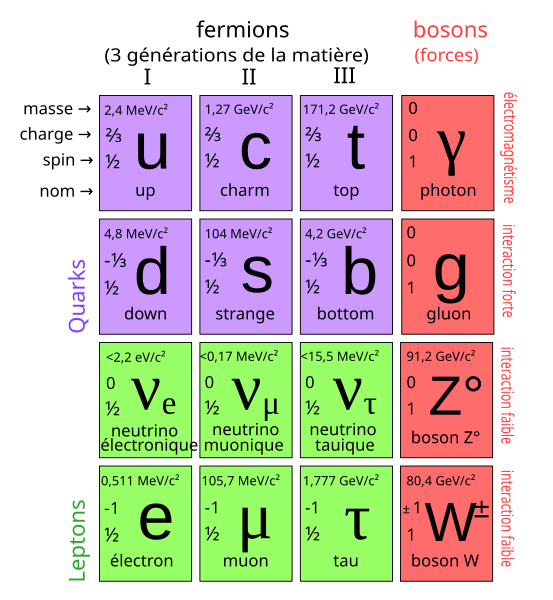
\includegraphics[width=0.5\linewidth]{img/ms.png}
    \caption{Particules élémentaires décrites par le Modèle Standard \cite{pdg2024}.}
    \label{fig:SM}
\end{figure}

\section{Constituants fondamentaux}

Les particules du Modèle Standard se répartissent en deux grandes catégories : les fermions, constituants de la matière, et les bosons, médiateurs des interactions.

\subsection{Fermions}

Les fermions de spin \(1/2\) obéissent à la statistique de Fermi-Dirac. Ils se divisent en :

\begin{itemize}
    \item \textbf{Leptons} : électron \(e\), muon \(\mu\), tau \(\tau\) et leurs neutrinos associés ;
    \item \textbf{Quarks} : \(u,\,d,\,c,\,s,\,t,\,b\), porteurs de charge de couleur et soumis à l'interaction forte.
\end{itemize}

Ils sont organisés en trois générations de masses croissantes. La matière ordinaire est essentiellement constituée des fermions de première génération.

\subsection{Bosons de jauge}

Les interactions fondamentales sont médiées par des bosons de spin 1 :

\begin{itemize}
    \item photon \(\gamma\) : interaction électromagnétique ;
    \item bosons \(W^\pm\) et \(Z^0\) : interaction faible \cite{pdg2024} ;
    \item gluons : interaction forte.
\end{itemize}

\subsection{Boson de Higgs}

Le boson de Higgs est une particule scalaire de spin 0, responsable de la brisure spontanée de la symétrie électrofaible et de la génération des masses des particules.

\section{Hadrons et interaction forte}

Dans le contexte de la calorimétrie hadronique, les particules observées expérimentalement sont principalement des états liés de quarks, appelés hadrons.

La QCD décrit l'interaction forte entre quarks et gluons. Elle est caractérisée par deux propriétés fondamentales \cite{PeskinSchroeder1995} :

\begin{itemize}
    \item \textbf{Confinement de couleur} : les quarks ne sont jamais observés isolément ;
    \item \textbf{Liberté asymptotique} : le couplage fort diminue à haute énergie.
\end{itemize}

On distingue principalement deux familles d'hadrons \cite{pdg2024} :

\begin{itemize}
    \item \textbf{Baryons} (\(qqq\)) : proton, neutron, etc. ;
    \item \textbf{Mésons} (\(q\bar{q}\)) : pions, kaons, etc.
\end{itemize}

Leur interaction avec la matière absorbante repose sur des processus nucléaires inélastiques complexes, à l'origine du développement des gerbes hadroniques dans les calorimètres.

\section{Particules d'intérêt de cette étude}

Dans ce travail, nous nous concentrons sur trois espèces hadroniques représentatives, choisies pour leurs signatures calorimétriques distinctes.

Leurs propriétés fondamentales sont résumées dans le Tableau~\ref{tab:hadrons}.

\begin{table}[!ht]
    \centering
    \caption{Propriétés des hadrons étudiés \cite{pdg2024}.}
    \label{tab:hadrons}
    \begin{tabular}{lccccl}
        \hline
        \textbf{Particule} & \textbf{Symbole} & \textbf{Masse (MeV)} &
        \textbf{Charge} & \textbf{Temps de vie} & \textbf{Contenu en quarks} \\
        \hline
        Pion chargé  & \(\pi^-\)  & 139.57  & \(-1\) & \(26.0\)~ns   & \(\bar{u}d\)                        \\
        Proton       & \(p\)      & 938.27  & \(+1\) & stable        & \(uud\)                             \\
        Kaon neutre long & \(K^0_L\) & 497.61 & \(0\) & \(51.2\)~ns  & \(\frac{1}{\sqrt{2}}(d\bar{s}-s\bar{d})\) \\
        \hline
    \end{tabular}
\end{table}

Ces particules présentent des comportements différents dans un calorimètre :

\begin{itemize}
    \item \textbf{Les pions} produisent des gerbes avec une composante électromagnétique significative via la production de \(\pi^0\) ;
    \item \textbf{Les protons} génèrent des gerbes plus hadroniques et généralement plus profondes ;
    \item \textbf{Les kaons neutres longs} n'ionisent pas avant leur première interaction et présentent des signatures distinctes liées à leur étrangeté.
\end{itemize}

La séparation de ces espèces constitue le problème central d'identification de particules (PID) étudié dans ce mémoire.

\section{Lien avec la calorimétrie hadronique}

Dans les expériences de physique des hautes énergies, une fraction importante de l'énergie finale est transportée par des hadrons organisés en jets. La mesure précise de ces jets repose de manière déterminante sur les calorimètres hadroniques.

Les gerbes hadroniques présentent des fluctuations importantes liées aux processus nucléaires inélastiques, à l'énergie invisible et aux fuites, ce qui dégrade la résolution énergétique. Ces limitations constituent une motivation centrale pour le développement de calorimètres à haute granularité.

Le \emph{Semi-Digital Hadron CALorimeter} (SDHCAL), développé au sein de la collaboration CALICE, s'inscrit dans cette approche. Sa granularité fine et sa lecture multi-seuils permettent d'exploiter la structure des gerbes hadroniques de manière détaillée, ouvrant la voie à des méthodes avancées d'identification des particules et de reconstruction d'énergie.
\chapter{Interactions particule--matière et développement des gerbes}
\label{sec:interactions}

La réponse d'un détecteur calorimétrique repose directement sur les mécanismes d'interaction entre
les particules incidentes et la matière absorbante. Selon leur nature, leur charge et leur énergie,
ces particules déposent leur énergie par ionisation, rayonnement ou interactions nucléaires, donnant
naissance à des cascades secondaires appelées \textbf{gerbes}. La compréhension de ces phénomènes
est essentielle pour interpréter la réponse du SDHCAL et améliorer les performances de
reconstruction étudiées dans ce mémoire.

% ─────────────────────────────────────────────────────────────────────────────
\section{Interaction des particules avec la matière}
\label{sec:interactions-matiere}

\subsection{Interactions des particules chargées}

Dans un milieu, une particule chargée perd principalement de l'énergie par \textbf{ionisation} et
\textbf{excitation} des atomes. La dépendance moyenne du pouvoir d'arrêt suit la loi de
Bethe--Bloch \cite{bichsel1988, pdg2024} :

\begin{equation}
\left\langle -\frac{\mathrm{d}E}{\mathrm{d}x} \right\rangle
= K\,z^{2}\,\frac{Z}{A}\,\frac{1}{\beta^{2}}
\left[
\frac{1}{2}\ln\!\left(
\frac{2 m_{e} c^{2}\,\beta^{2}\gamma^{2}\,T_{\max}}{I^{2}}
\right)
- \beta^{2} - \frac{\delta}{2}
\right],
\label{eq:bethe-bloch}
\end{equation}

où $K = 4\pi N_A r_e^2 m_e c^2$, $z$ est la charge de la particule incidente, $Z/A$ le rapport
charge/masse du milieu, $I$ le potentiel moyen d'excitation, $T_{\max}$ l'énergie maximale
transférable à un électron libre et $\delta$ le terme de correction de densité \cite{pdg2024}.

Cette expression présente un \textit{minimum d'ionisation} pour $\beta\gamma \simeq 3$--$4$
(régime de la particule au minimum d'ionisation, MIP). Dans la gamme d'énergies considérée pour
le SDHCAL (1--130~GeV), l'ionisation domine pour les hadrons et les muons, ce qui justifie l'usage
du MIP comme unité de calibration et motive la lecture multi-seuils pour caractériser la densité
locale de dépôt.

Les autres mécanismes sont secondaires dans ce contexte :

\begin{itemize}
    \item \textbf{Bremsstrahlung} : dominant seulement pour $e^\pm$ au-delà de l'énergie critique
          $E_c \sim 500/Z$~MeV ; négligeable pour hadrons et muons aux énergies visées.
    \item \textbf{Diffusions $e$--$e$} (Møller/Bhabha) et annihilation $e^+$ : effets spécifiques
          aux $e^\pm$, marginaux pour la calorimétrie hadronique étudiée ici.
\end{itemize}

\subsection{Interactions des photons}

Les photons interagissent avec la matière via trois processus principaux, dont l'importance relative
dépend de leur énergie \cite{pdg2024} :

\begin{itemize}
    \item à \textbf{basse énergie} (keV), l'\textit{effet photoélectrique} domine ;
    \item aux \textbf{énergies intermédiaires} (quelques MeV), la \textit{diffusion Compton}
          est prépondérante ;
    \item à \textbf{haute énergie} ($\gg 2 m_e c^2$), la \textit{création de paires}
          $\gamma \to e^+e^-$ devient dominante.
\end{itemize}

Dans un calorimètre comme le SDHCAL, ces mécanismes contribuent essentiellement à la composante
électromagnétique des gerbes, notamment via la désintégration $\pi^0 \to \gamma\gamma$.

\subsection{Interactions des hadrons et des neutrons}

Comme les électrons, les hadrons chargés perdent d'abord de l'énergie par ionisation. Mais, soumis
à l'\textbf{interaction forte}, leurs processus d'interaction sont beaucoup plus complexes.

Lorsqu'un hadron incident interagit avec un noyau, il déclenche une \textbf{spallation nucléaire}
\cite{knoll2010, wigmans2000}. Celle-ci se déroule en deux étapes :

\begin{enumerate}
    \item \textbf{Cascade intranucléaire} : le hadron interagit avec un ou plusieurs nucléons,
          induisant des collisions secondaires. Des hadrons supplémentaires peuvent être créés ;
          certains s'échappent du noyau, d'autres sont réabsorbés.
    \item \textbf{Désexcitation du noyau} : évaporation de protons, neutrons et particules
          $\alpha$, suivie d'émission de $\gamma$. Dans les noyaux lourds, la fission est possible.
\end{enumerate}

Ce processus est hautement stochastique. Une fraction de l'énergie reste \textbf{invisible aux
calorimètres} :

\begin{itemize}
    \item énergie de liaison nucléaire consommée lors de la spallation ;
    \item énergie cinétique de recul du noyau résiduel ;
    \item neutrons secondaires faiblement ou tardivement détectés.
\end{itemize}

Les \textbf{hadrons neutres} (comme le $K^0_L$) n'ionisent pas et ne déposent de l'énergie que via
ces interactions nucléaires, ce qui rend leur point de départ de gerbe plus variable.

Les \textbf{neutrons} constituent un cas particulier selon leur énergie \cite{knoll2010} :

\begin{itemize}
    \item \textbf{Diffusion élastique} ($E < 1$--$10$~MeV) : transfert d'énergie cinétique aux
          noyaux, efficace sur l'hydrogène, mais induisant des signaux retardés ou délocalisés.
    \item \textbf{Diffusion inélastique} ($10$--$100$~MeV) : excitation du noyau suivie
          d'émissions $\gamma$, $p$, $n$, $\alpha$, voire fission.
    \item \textbf{Capture radiative} ($E \approx 0$) : absorption par le noyau, désexcitation
          par $\gamma$ ou $\alpha$.
\end{itemize}

La déposition d'énergie des hadrons dans un calorimètre combine donc des processus d'ionisation,
d'interactions fortes et de cascades nucléaires, avec une forte variabilité et une part d'énergie
non détectée. Ces effets expliquent la complexité de la réponse des calorimètres hadroniques et
les difficultés à atteindre une résolution comparable à celle des calorimètres
électromagnétiques \cite{fabjan2003, wigmans2000}.

% ─────────────────────────────────────────────────────────────────────────────
\section{Gerbes électromagnétiques}
\label{sec:gerbes-em}

Les gerbes électromagnétiques (EM) sont initiées par des électrons, des photons, ou par des
$\pi^0 \to \gamma\gamma$ \cite{heitler1954, rossi1952}. Elles résultent de l'alternance entre
\textit{bremsstrahlung} ($e^\pm \to e^\pm\gamma$) et \textit{création de paires}
($\gamma \to e^+e^-$), jusqu'à ce que l'énergie descende sous l'énergie critique $E_c$, où
l'ionisation devient dominante.

La structure longitudinale et transverse des gerbes est caractérisée par deux grandeurs
fondamentales \cite{pdg2024} :

\begin{itemize}
    \item la \textbf{longueur de radiation} $X_0$, définie comme la distance sur laquelle un
          électron perd en moyenne $1/e$ de son énergie par bremsstrahlung, et qui fixe l'échelle
          longitudinale de développement ;
    \item le \textbf{rayon de Molière} $R_M \approx 21\,\mathrm{MeV}\cdot X_0 / E_c$, qui définit
          l'extension transverse (environ 90\% de l'énergie est contenue dans un cylindre de
          rayon $R_M$).
\end{itemize}

Le profil longitudinal d'énergie déposée peut être décrit par \cite{pdg2024} :

\begin{equation}
\frac{\mathrm{d}E}{\mathrm{d}t} = E_0\,b\,\frac{(bt)^{a-1} e^{-bt}}{\Gamma(a)},
\label{eq:longitudinal-em}
\end{equation}

où $t = x/X_0$ est la profondeur réduite et les paramètres $a$, $b$ dépendent du matériau et de
l'énergie incidente. La position du maximum est donnée par $t_{\max} = (a-1)/b$.

Les gerbes électromagnétiques constituent une référence utile : leur développement est compact,
régulier et bien modélisé, contrairement aux gerbes hadroniques.

% ─────────────────────────────────────────────────────────────────────────────
\section{Gerbes hadroniques}
\label{sec:gerbes-had}

Lorsqu'un hadron de haute énergie pénètre dans un matériau absorbant, il initie une
\textbf{gerbe hadronique} — une cascade complexe de particules secondaires résultant d'interactions
nucléaires successives. Contrairement aux gerbes électromagnétiques, les gerbes hadroniques
présentent d'importantes fluctuations événement par événement dans leur composition, leur extension
spatiale et la fraction d'énergie effectivement détectée \cite{wigmans2000, fabjan2003}.

\subsection{Développement de la cascade}

La gerbe débute par une interaction inélastique du hadron incident avec un noyau du milieu,
produisant pions chargés et neutres, kaons, nucléons secondaires et fragments nucléaires. Les
hadrons secondaires suffisamment énergétiques alimentent la cascade en interagissant à leur tour.

Une caractéristique essentielle est la production de $\pi^0$, qui se désintègrent quasi
instantanément :

\[
\pi^0 \rightarrow \gamma\gamma,
\]

initiant des sous-gerbes électromagnétiques imbriquées. La fraction d'énergie dérivée vers cette
composante EM fluctue fortement d'un événement à l'autre et constitue la principale source de
variabilité de la réponse calorimétrique.

\subsection{Longueur d'interaction}

La grandeur gouvernant le développement longitudinal est la \textbf{longueur d'interaction
nucléaire} \cite{pdg2024} :

\begin{equation}
\lambda_I = \frac{A}{N_A\,\rho\,\sigma_{\mathrm{inel}}},
\label{eq:lambda-i}
\end{equation}

où $A$ est la masse molaire du matériau, $\rho$ sa densité, $N_A$ le nombre d'Avogadro et
$\sigma_{\mathrm{inel}}$ la section efficace inélastique hadron-noyau. Dans les matériaux denses
typiques, $\lambda_I \gg X_0$ : les gerbes hadroniques sont plus profondes et plus diffuses que
les gerbes électromagnétiques, imposant des calorimètres plus épais et moins bien contenus.

\begin{table}[!ht]
    \centering
    \caption{Comparaison des longueurs caractéristiques pour quelques matériaux d'absorbeur
             courants \cite{pdg2024}.}
    \label{tab:longueurs-carac}
    \begin{tabular}{lcccc}
        \hline
        \textbf{Matériau} & $Z$ & $X_0$ (cm) & $\lambda_I$ (cm) & $\lambda_I / X_0$ \\
        \hline
        Fer (Fe)      & 26 & 1.76  & 16.77 & 9.5  \\
        Plomb (Pb)    & 82 & 0.56  & 17.59 & 31.4 \\
        Acier inox    & -- & 1.76  & 16.77 & 9.5  \\
        Tungstène (W) & 74 & 0.35  & 9.95  & 28.4 \\
        \hline
    \end{tabular}
\end{table}

\noindent Le Tableau~\ref{tab:longueurs-carac} illustre le fait que, quelle que soit la densité du
matériau, $\lambda_I$ reste toujours bien supérieure à $X_0$, justifiant la profondeur importante
requise pour les calorimètres hadroniques.

\subsection{Fraction électromagnétique et rapport \texorpdfstring{$h/e$}{h/e}}

La fraction d'énergie transférée à la composante EM via la production de $\pi^0$ est appelée
\textbf{fraction électromagnétique} :

\[
f_{\mathrm{em}} = \frac{E_{\mathrm{EM}}}{E_{\mathrm{tot}}}.
\]

En moyenne, $\langle f_{\mathrm{em}} \rangle$ croît avec l'énergie incidente selon une loi
approximative \cite{wigmans2000} :

\begin{equation}
\langle f_{\mathrm{em}} \rangle \approx 1 - \left(\frac{E}{E_0}\right)^{m-1},
\label{eq:fem}
\end{equation}

avec $E_0$ et $m$ des paramètres dépendant du matériau et de l'espèce hadronique. Toutefois,
$f_{\mathrm{em}}$ fluctue fortement d'un événement à l'autre, même à énergie fixée.

La réponse moyenne d'un calorimètre à une gerbe hadronique s'écrit \cite{wigmans2000} :

\begin{equation}
\langle E_{\pi}\rangle = \left[f_{\mathrm{em}} + (1 - f_{\mathrm{em}})\,\frac{h}{e}\right] E,
\label{eq:he}
\end{equation}

où $e$ et $h$ désignent respectivement les réponses électromagnétique et hadronique du détecteur.
Un calorimètre est dit \textbf{compensant} lorsque $h/e = 1$, ce qui minimise les effets des
fluctuations de $f_{\mathrm{em}}$ sur la résolution. Hors compensation, ces fluctuations constituent
la contribution dominante à la non-linéarité et à la dégradation de la résolution énergétique.

\subsection{Énergie invisible}

Une fraction de l'énergie incidente n'est pas convertie en signal mesurable \cite{fabjan2003} :

\begin{itemize}
    \item énergie de liaison nucléaire consommée lors de la spallation ;
    \item énergie cinétique de recul des noyaux résiduels ;
    \item neutrons secondaires peu ou tardivement détectés ;
    \item particules pénétrantes (muons, neutrinos produits dans certaines désintégrations).
\end{itemize}

Cette énergie invisible est intrinsèquement variable d'un événement à l'autre et contribue
directement à la dégradation de la résolution.

\subsection{Effets temporels}

Les cascades hadroniques ont une structure temporelle plus étendue que les gerbes
électromagnétiques. Une partie du signal est déposée rapidement par les particules relativistes,
tandis que d'autres contributions apparaissent plus tardivement via les neutrons ralentis puis
capturés (temps caractéristiques de l'ordre de quelques dizaines de nanosecondes).

La réponse mesurée dépend donc directement de la fenêtre temporelle d'acquisition du détecteur.
Cet aspect est particulièrement pertinent pour le SDHCAL, dont la lecture semi-digitale est
sensible à la chronologie des dépôts, et dont les variables temporelles constituent des
descripteurs potentiellement discriminants pour le PID (voir chapitre~\ref{sec:pid_mlp}).

\subsection{Containment et fluctuations}

Les gerbes hadroniques, en raison de leur grande extension longitudinale et transverse, peuvent
ne pas être totalement contenues dans le volume instrumenté. L'énergie qui s'échappe crée des
\textbf{fuites longitudinales ou latérales} qui s'ajoutent aux autres sources de dégradation.

La paramétrisation standard de la résolution énergétique d'un calorimètre hadronique est
\cite{fabjan2003} :

\begin{equation}
\frac{\sigma(E)}{E} = \frac{a}{\sqrt{E/\mathrm{GeV}}} \oplus b \oplus \frac{c}{E/\mathrm{GeV}},
\label{eq:resolution}
\end{equation}

où $a$ est le terme stochastique (dominé par les fluctuations de $f_{\mathrm{em}}$ et les
fluctuations d'échantillonnage), $b$ le terme constant (effets systématiques, non-uniformités,
fuites) et $c$ le terme de bruit électronique. L'amélioration de la résolution passe avant tout
par la maîtrise du terme $a$, c'est-à-dire par la réduction des effets liés aux fluctuations
hadroniques.

\subsection{Profils spatiaux}

Le profil longitudinal d'une gerbe hadronique présente une montée rapide suivie d'une décroissance
lente. Son profil transverse se compose de :

\begin{itemize}
    \item un \textbf{cœur dense}, enrichi en composante électromagnétique ($\pi^0 \to \gamma\gamma$),
          de rayon caractéristique proche de $R_M$ ;
    \item une \textbf{région périphérique diffuse}, dominée par les hadrons secondaires et les
          neutrons, s'étendant jusqu'à plusieurs $\lambda_I$ transversalement.
\end{itemize}

\begin{figure}[!ht]
    \centering
    \begin{tikzpicture}[scale=1.05]

        %% ── Axes du profil longitudinal ────────────────────────────────────
        \draw[->, thick] (0,0) -- (7.5,0)
            node[right, font=\small] {Profondeur ($\lambda_I$)};
        \draw[->, thick] (0,0) -- (0,4.2)
            node[above, font=\small] {$\mathrm{d}E/\mathrm{d}x$ (u.a.)};

        %% ── Gerbe hadronique ───────────────────────────────────────────────
        \draw[thick, blue!70!black]
            plot[smooth, tension=0.6] coordinates
            {(0,0)(0.6,0.8)(1.2,2.4)(1.8,3.4)(2.4,3.6)(3.0,3.3)
             (3.8,2.7)(4.8,1.8)(5.8,1.0)(6.8,0.4)(7.2,0.15)};
        \node[blue!70!black, font=\small] at (5.5,3.1)
            {Gerbe hadronique};

        %% ── Gerbe électromagnétique ─────────────────────────────────────
        \draw[thick, red!70!black, dashed]
            plot[smooth, tension=0.7] coordinates
            {(0,0)(0.4,1.2)(0.8,3.0)(1.1,3.8)(1.4,3.2)
             (1.9,1.8)(2.6,0.7)(3.5,0.2)(4.0,0.05)};
        \node[red!70!black, font=\small] at (3.0,3.5)
            {Gerbe EM};

        %% ── Annotations longueurs caractéristiques ───────────────────────
        \draw[<->, gray] (0,-0.5) -- (1.1,-0.5)
            node[midway, below, font=\tiny] {$\sim\! X_0$};
        \draw[<->, gray] (0,-1.0) -- (3.0,-1.0)
            node[midway, below, font=\tiny] {$\sim\! \lambda_I$};

    \end{tikzpicture}

    \vspace{0.8em}

    \begin{tikzpicture}[scale=1.05]

        %% ── Vue transversale ───────────────────────────────────────────────
        \draw[->, thick] (-3.5,0) -- (3.5,0)
            node[right, font=\small] {Rayon transverse};
        \draw[->, thick] (0,-0.3) -- (0,3.8)
            node[above, font=\small] {Densité d'énergie (u.a.)};

        %% ── Composante EM (cœur compact) ──────────────────────────────────
        \fill[red!20]
            plot[smooth, tension=0.8] coordinates
            {(-1.0,0)(-0.8,0.6)(-0.4,2.2)(0,2.9)(0.4,2.2)(0.8,0.6)(1.0,0)}
            -- cycle;
        \draw[thick, red!70!black]
            plot[smooth, tension=0.8] coordinates
            {(-1.0,0)(-0.8,0.6)(-0.4,2.2)(0,2.9)(0.4,2.2)(0.8,0.6)(1.0,0)};
        \node[red!70!black, font=\small] at (1.8,2.8)
            {Cœur EM ($\sim\!R_M$)};

        %% ── Halo hadronique ───────────────────────────────────────────────
        \fill[blue!10]
            plot[smooth, tension=0.6] coordinates
            {(-3.2,0)(-2.5,0.3)(-2.0,0.7)(-1.2,0.9)(-0.8,0.6)
             (-0.4,2.2)(0,2.9)(0.4,2.2)(0.8,0.6)(1.2,0.9)
             (2.0,0.7)(2.5,0.3)(3.2,0)}
            -- cycle;
        \draw[thick, blue!70!black]
            plot[smooth, tension=0.6] coordinates
            {(-3.2,0)(-2.5,0.3)(-2.0,0.7)(-1.2,0.9)(-0.8,0.6)
             (-0.4,2.2)(0,2.9)(0.4,2.2)(0.8,0.6)(1.2,0.9)
             (2.0,0.7)(2.5,0.3)(3.2,0)};
        \node[blue!70!black, font=\small] at (-2.3,1.5)
            {Halo hadronique};

        %% ── Annotation R_M ────────────────────────────────────────────────
        \draw[<->, gray] (0,-0.25) -- (1.0,-0.25)
            node[midway, below, font=\tiny] {$R_M$};

    \end{tikzpicture}

    \caption{Haut : profils longitudinaux comparés d'une gerbe hadronique (bleu) et
             électromagnétique (rouge pointillé). Les échelles caractéristiques $X_0$ et
             $\lambda_I$ sont indiquées. Bas : profil transverse d'une gerbe hadronique montrant
             le cœur électromagnétique compact (rouge) et le halo hadronique étendu (bleu).}
    \label{fig:profils-gerbes}
\end{figure}

La Figure~\ref{fig:profils-gerbes} illustre ces différences. L'étude fine de ces profils, rendue
possible par la haute granularité du SDHCAL, constitue la base des méthodes d'identification
hadronique développées dans ce mémoire.

\subsection{Lien avec cette étude}

L'ensemble des effets décrits dans ce chapitre motive directement le développement du SDHCAL et
l'usage de méthodes d'apprentissage automatique pour l'analyse des gerbes. Les fluctuations de
$f_{\mathrm{em}}$, les profils spatiaux différenciés selon l'espèce et la structure temporelle
des dépôts constituent autant d'observables exploitables pour le PID et la reconstruction
d'énergie — à condition de disposer d'un calorimètre suffisamment granulaire pour les mesurer
finement.

\chapter{Identification hadronique : physique et enjeux expérimentaux}
\label{chap:pid_physique}

Ce chapitre précise les raisons physiques et expérimentales qui motivent l'identification hadronique dans le SDHCAL. Après avoir rappelé l'intérêt du PID, nous discutons les différences attendues entre pions, protons et kaons neutres longs, puis les conséquences de cette séparation pour la reconstruction calorimétrique.

\section{Pourquoi distinguer les hadrons ?}

L'identification des particules (\emph{Particle Identification}, PID) constitue une étape importante dans les expériences de physique des hautes énergies. Dans les états finals hadroniques, les particules produites forment souvent des jets issus de la fragmentation de quarks et de gluons. Une mauvaise identification des espèces peut conduire à une association incorrecte des dépôts d'énergie, à une calibration inadéquate ou à une dégradation de la résolution globale \cite{pdg2024}.

Le besoin de PID apparaît aussi dans les campagnes de faisceaux-tests. Les faisceaux secondaires utilisés pour calibrer les calorimètres ne sont pas parfaitement purs : un faisceau nominalement composé de pions peut contenir des protons, des muons ou d'autres composantes parasites. Si toutes les particules sont traitées comme une seule espèce de référence, la réponse moyenne du détecteur peut être biaisée.

Dans le cas du SDHCAL, la haute granularité spatiale et la lecture semi-digitale à trois seuils fournissent une information plus riche qu'un simple signal intégré. La morphologie tridimensionnelle des gerbes devient alors exploitable pour différencier les espèces hadroniques événement par événement.

\section{Différences physiques entre pions, protons et kaons neutres longs}
\label{sec:differences-physiques}

Les trois espèces étudiées présentent des propriétés fondamentales différentes, résumées dans le Tableau~\ref{tab:proprietes-pid}. Ces différences influencent leur mode d'interaction avec la matière et donc la structure moyenne de leurs gerbes.

\begin{table}[!ht]
    \centering
    \caption{Propriétés fondamentales des trois espèces hadroniques étudiées et conséquences calorimétriques attendues \cite{pdg2024}.}
    \label{tab:proprietes-pid}
    \renewcommand{\arraystretch}{1.35}
    \begin{tabularx}{\textwidth}{lccc>{\raggedright\arraybackslash}X}
        \hline
        \textbf{Espèce} & \textbf{Masse} & \textbf{Charge} & \textbf{Nature} &
        \textbf{Conséquence principale} \\
        \hline
        $\pi^-$   & 139.6~MeV & $-1$ & Méson   &
            Ionisation initiale ; composante EM souvent marquée \\
        $p$       & 938.3~MeV & $+1$ & Baryon  &
            Gerbe plus hadronique et plus profonde \\
        $K^0_L$   & 497.6~MeV & $0$  & Méson neutre &
            Pas d'ionisation initiale ; départ de gerbe variable \\
        \hline
    \end{tabularx}
\end{table}

\subsection{Pions chargés \texorpdfstring{$\pi^-$}{pi-}}

Les pions chargés sont des mésons légers. Avant leur première interaction nucléaire, ils déposent de l'énergie par ionisation dans les premières couches du calorimètre. Lors du développement de la gerbe, la production de pions neutres secondaires, suivie de la désintégration $\pi^0 \to \gamma\gamma$, alimente la composante électromagnétique de la cascade. Les gerbes de pions présentent ainsi souvent un développement relativement précoce et un cœur électromagnétique marqué.

\subsection{Protons \texorpdfstring{$p$}{p}}

Les protons sont des baryons stables de masse plus élevée. Leur nature baryonique modifie la dynamique de la cascade, notamment à travers la conservation du nombre baryonique. À énergie identique, leurs gerbes tendent en moyenne à être plus hadroniques, plus profondes et plus diffuses que celles des pions, avec une fraction électromagnétique généralement plus faible.

\subsection{Kaons neutres longs \texorpdfstring{$K^0_L$}{KL0}}

Les kaons neutres longs ne portent pas de charge électrique. Ils ne déposent donc pas d'énergie par ionisation avant leur première interaction nucléaire. Le point de départ de leur gerbe est gouverné par leur libre parcours moyen dans le matériau, ce qui rend leur développement longitudinal plus variable. Leur contenu en étrangeté implique également des voies de réaction différentes de celles des pions et des protons.

\section{Signatures calorimétriques attendues}
\label{sec:comparaison-signatures}

Les différences de masse, de charge et de structure interne se traduisent par des signatures calorimétriques moyennes distinctes. Ces tendances restent statistiques, car les gerbes hadroniques présentent de fortes fluctuations événement par événement.

\begin{table}[!ht]
    \centering
    \caption{Comparaison qualitative des signatures calorimétriques moyennes attendues dans le SDHCAL.}
    \label{tab:comparaison-signatures}
    \renewcommand{\arraystretch}{1.4}
    \resizebox{\textwidth}{!}{%
    \begin{tabular}{lccc}
        \hline
        \textbf{Caractéristique} &
        \textbf{Pion $\pi^-$} &
        \textbf{Proton $p$} &
        \textbf{Kaon neutre long $K^0_L$} \\
        \hline
        Signal d'ionisation avant gerbe    & Oui               & Oui               & Non \\
        Fraction électromagnétique moyenne & Élevée            & Plus faible       & Variable \\
        Profondeur de première interaction & Plutôt précoce    & Plutôt précoce    & Plus variable \\
        Développement longitudinal         & Relativement précoce & Plus profond   & Variable \\
        Extension transverse               & Modérée           & Plus large        & Variable \\
        Fluctuations événement/événement   & Importantes       & Importantes       & Très importantes \\
        \hline
    \end{tabular}%
    }
\end{table}

Ces différences suggèrent que des observables de morphologie, telles que le profil longitudinal, la compacité transverse, la profondeur du premier dépôt ou la répartition entre seuils, peuvent porter une information discriminante exploitable pour le PID.

\section{Conséquences pour la reconstruction calorimétrique}
\label{sec:consequences-reco}

L'identification de l'espèce incidente ne constitue pas seulement un problème de classification. Elle peut également améliorer la reconstruction de l'énergie.

En effet, si deux espèces présentent des réponses moyennes différentes dans le calorimètre, l'application d'une calibration unique introduit un biais. Une calibration ajustée sur des pions peut par exemple ne pas être optimale pour des protons ou des kaons. Le PID permet alors de router les événements vers une calibration adaptée à l'espèce prédite, ou au minimum de mieux contrôler les effets liés aux mélanges d'espèces.

Dans ce travail, cette idée est étudiée à travers trois scénarios :

\begin{enumerate}[label=(\roman*)]
    \item une calibration pion appliquée à toutes les espèces ;
    \item une calibration assistée par PID, utilisant la classe prédite ;
    \item une calibration idéale, utilisant la vérité issue de la simulation.
\end{enumerate}

Cette comparaison permet d'évaluer quantitativement dans quelle mesure le PID peut rapprocher la reconstruction réelle d'une situation idéale où l'espèce incidente serait parfaitement connue.

\section{Lien avec le SDHCAL}
\label{sec:lien-sdhcal-pid}

Le SDHCAL est particulièrement adapté à cette problématique grâce à sa granularité fine et à sa lecture semi-digitale. Ces caractéristiques donnent accès à plusieurs familles d'observables :

\begin{itemize}
    \item observables longitudinales : profondeur du premier dépôt, position du maximum, extension de la gerbe ;
    \item observables transverses : compacité, rayon effectif, dispersion spatiale ;
    \item observables de densité : nombre de hits, répartition entre les seuils 1, 2 et 3 ;
    \item observables temporelles éventuelles : distribution des temps de dépôt.
\end{itemize}

L'exploitation conjointe de ces informations par des méthodes d'apprentissage supervisé constitue le cœur de l'étude d'identification hadronique présentée dans la suite du mémoire.

\section{Conclusion}
\label{sec:conclusion-pid-physique}

La séparation entre pions, protons et kaons neutres longs repose sur des différences physiques réelles : charge électrique, masse, nature mésonique ou baryonique, et dynamique d'interaction hadronique. Ces différences se traduisent par des signatures calorimétriques distinctes, notamment sur le développement longitudinal, la compacité transverse et la fraction électromagnétique moyenne.

Cependant, les fortes fluctuations des gerbes hadroniques rendent cette séparation non triviale. Les signatures des différentes espèces se recouvrent partiellement, ce qui justifie l'utilisation de méthodes multivariées et d'apprentissage automatique capables d'exploiter simultanément plusieurs observables de gerbe.

\chapter{Le calorimètre SDHCAL}
\label{chap:sdhcal}

\section{Motivation du concept SDHCAL}

Le \emph{Semi-Digital Hadron CALorimeter} (SDHCAL) est un calorimètre hadronique hautement granulaire développé dans le cadre de la collaboration CALICE. Il s'inscrit dans le contexte des futurs détecteurs de physique des hautes énergies, où la reconstruction précise des jets impose une excellente séparation spatiale des particules et une mesure fiable des gerbes hadroniques.

Contrairement aux calorimètres hadroniques conventionnels, le SDHCAL ne repose pas uniquement sur une mesure globale de l'énergie déposée. Son principe consiste à exploiter la structure tridimensionnelle des gerbes, grâce à une segmentation fine et à une lecture semi-digitale. Cette approche est particulièrement adaptée aux algorithmes de type \emph{Particle Flow Algorithm} et aux méthodes modernes d'identification des particules.

Le concept du SDHCAL repose sur deux éléments principaux :

\begin{enumerate}
    \item une granularité spatiale fine, permettant une imagerie détaillée des gerbes ;
    \item une lecture à trois seuils, conservant une information sur la densité locale des dépôts.
\end{enumerate}

Cette combinaison permet de conserver une information riche sur la morphologie des gerbes, tout en limitant la complexité électronique par rapport à une lecture entièrement analogique.

\section{Géométrie générale du prototype}

Le prototype SDHCAL est un calorimètre à échantillonnage constitué de 48 couches actives insérées entre des plaques d'acier inoxydable de 2~cm d'épaisseur. L'ensemble correspond à une profondeur totale d'environ \(6\,\lambda_I\), permettant de contenir une grande partie des gerbes hadroniques dans la gamme d'énergie étudiée.

Chaque couche active couvre une surface de \(96 \times 96~\mathrm{cm}^2\) et est segmentée en pads de \(1 \times 1~\mathrm{cm}^2\). Chaque plan contient ainsi 9216 cellules indépendantes, ce qui donne accès à une image tridimensionnelle détaillée du développement des cascades.

Les détecteurs actifs utilisés sont des chambres résistives à plaques de verre, ou \emph{Glass Resistive Plate Chambers} (GRPC). Elles sont constituées de deux plaques de verre séparées par un faible entrefer gazeux, dans lequel se développe l'avalanche induite par le passage d'une particule chargée.

Les GRPC présentent plusieurs avantages pour un calorimètre hautement granulaire :

\begin{itemize}
    \item un coût modéré pour de grandes surfaces ;
    \item une bonne homogénéité spatiale ;
    \item une efficacité élevée pour les particules au minimum d'ionisation ;
    \item une compatibilité naturelle avec une lecture segmentée en pads.
\end{itemize}

\begin{figure}[!ht]
    \centering
    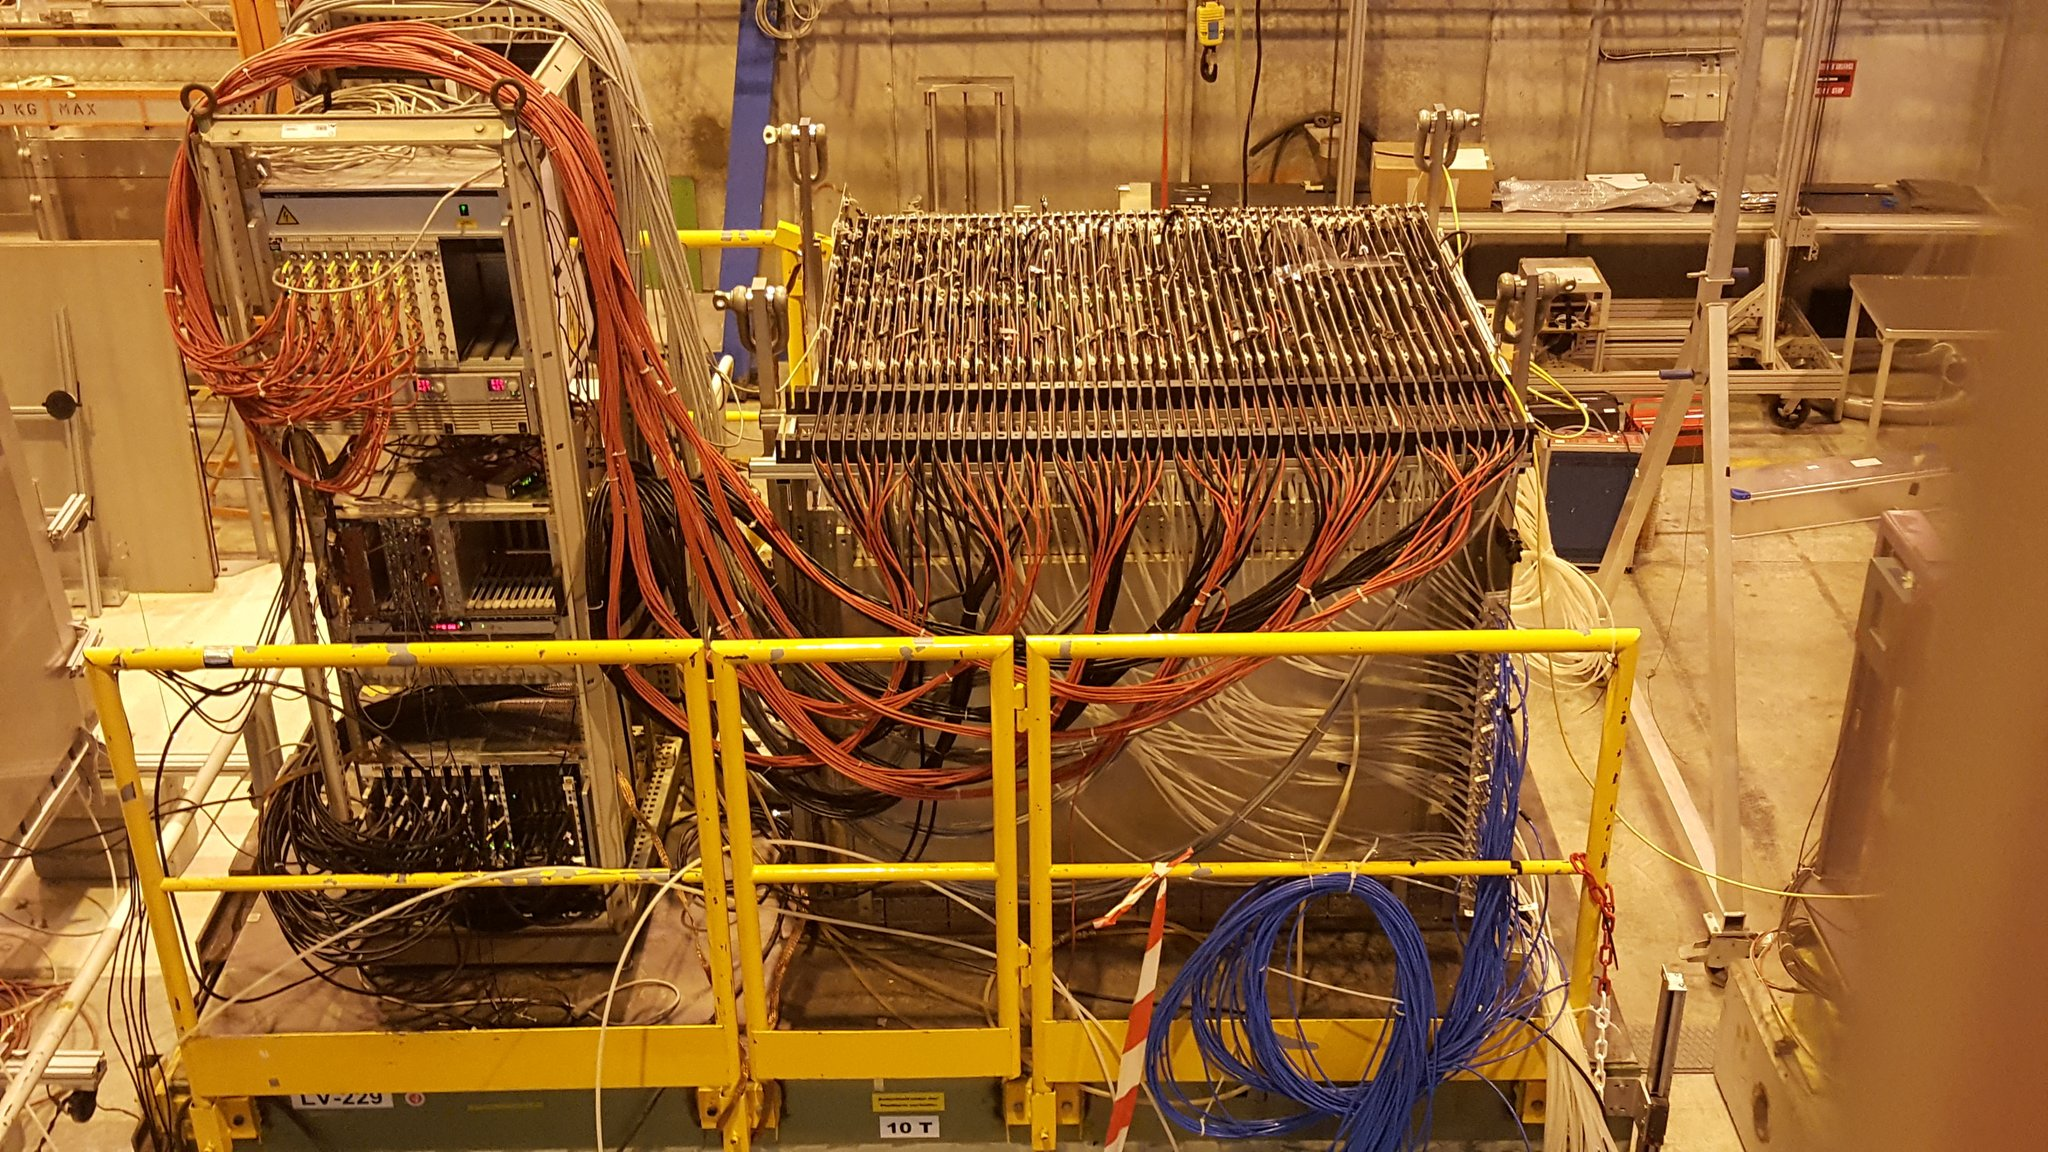
\includegraphics[width=0.8\linewidth]{Fig/sdhcal_prototype.jpeg}
    \caption{Vue du prototype SDHCAL instrumenté lors d'une campagne de test faisceau.}
    \label{fig:sdhcal_real}
\end{figure}

\section{Principe de détection dans les GRPC}

Lorsqu'une particule chargée traverse une GRPC, elle ionise le gaz contenu dans l'entrefer. Les électrons primaires produits sont accélérés par le champ électrique appliqué entre les plaques de verre, déclenchant une avalanche électronique.

Le signal induit est collecté sur les pads de lecture situés à proximité de l'anode. La charge mesurée dépend notamment du nombre d'ionisations initiales, de la position de passage de la particule, des conditions de champ électrique, de la composition du gaz et des fluctuations propres au processus d'avalanche.

Le mélange gazeux et les conditions de fonctionnement sont choisis afin d'assurer une avalanche stable, une efficacité élevée et une limitation des décharges de type streamer.

\section{Lecture semi-digitale à trois seuils}

L'originalité du SDHCAL réside dans sa lecture semi-digitale codée sur deux bits. Trois seuils de charge sont appliqués à chaque canal :

\begin{equation}
T_1 < T_2 < T_3.
\end{equation}

Chaque hit est classé selon le plus haut seuil franchi. Cette information permet de distinguer grossièrement les dépôts isolés, les régions de densité intermédiaire et les zones très denses de la gerbe.

Une lecture purement digitale fournirait uniquement une information de présence ou d'absence de hit, ce qui entraînerait une saturation dans les régions centrales des gerbes. À l'inverse, la lecture semi-digitale conserve une sensibilité à la densité locale tout en maintenant une électronique plus simple qu'une lecture analogique complète.

Les observables directement accessibles sont notamment :

\begin{itemize}
    \item le nombre total de hits ;
    \item les compteurs par seuil \(N_1\), \(N_2\), \(N_3\) ;
    \item les fractions relatives entre seuils ;
    \item les distributions spatiales des hits ;
    \item les densités locales de dépôt.
\end{itemize}

Ces informations constituent la base des méthodes de reconstruction d'énergie et d'identification hadronique étudiées dans ce mémoire.

\section{Électronique de lecture et acquisition}

L'électronique de lecture est intégrée au plus près des chambres grâce aux ASICs \textsc{HARDROC}, conçus pour les détecteurs gazeux hautement segmentés. Chaque ASIC gère plusieurs dizaines de canaux et dispose d'une mémoire locale permettant de stocker les informations avant la lecture.

Cette architecture embarquée réduit le câblage externe et rend possible l'instrumentation d'un très grand nombre de canaux. Le système peut fonctionner en mode déclenché ou en mode sans déclenchement, selon les conditions expérimentales.

Une stratégie de \emph{power pulsing} peut également être utilisée afin de réduire la consommation électrique pendant les périodes sans faisceau, un point important pour les futurs collisionneurs linéaires.

\section{Simulation et digitalisation}

L'étude présentée dans ce mémoire repose sur une chaîne de simulation basée sur l'environnement iLCSoft, utilisant Geant4 pour la propagation des particules dans le détecteur. La simulation fournit les dépôts d'énergie élémentaires dans les couches actives.

Une étape de digitalisation transforme ensuite ces dépôts physiques en hits comparables à ceux produits par l'électronique réelle. Cette étape inclut notamment :

\begin{enumerate}
    \item la sélection temporelle des dépôts ;
    \item l'application d'une efficacité de détection ;
    \item la génération d'une charge induite fluctuante ;
    \item la diffusion transverse vers les pads voisins ;
    \item l'application des trois seuils semi-digitaux ;
    \item la production des hits reconstruits.
\end{enumerate}

La sortie finale contient, pour chaque hit, ses coordonnées discrètes \((I,J,K)\), le seuil franchi, un horodatage et l'identifiant de l'événement. Ces données sont ensuite converties en formats d'analyse, notamment \texttt{ROOT} et \texttt{CSV}, pour les études de PID et de reconstruction énergétique.

\section{Validation expérimentale}

La simulation du SDHCAL doit reproduire les principales observables mesurées lors des campagnes de tests faisceau. Le prototype a notamment été étudié au CERN avec des faisceaux de muons, d'électrons et de hadrons sur une large gamme d'énergies.

La comparaison entre données et simulation porte sur plusieurs grandeurs :

\begin{itemize}
    \item le nombre total de hits par événement ;
    \item les distributions par seuil \(N_1\), \(N_2\), \(N_3\) ;
    \item l'efficacité MIP et la multiplicité des pads ;
    \item les profils longitudinaux des gerbes ;
    \item l'extension transverse ;
    \item la position du maximum de gerbe.
\end{itemize}

Ces comparaisons permettent d'ajuster les paramètres de digitalisation, de tester différentes listes de physique hadronique de Geant4 et d'estimer les incertitudes systématiques associées à la modélisation.

\section{Reconstruction de l'énergie}

Grâce à l'information multi-seuil, l'énergie incidente peut être estimée à partir d'une combinaison pondérée des compteurs de hits :

\begin{equation}
E_{\mathrm{reco}}
=
a(N_{\mathrm{tot}})N_1
+
b(N_{\mathrm{tot}})N_2
+
c(N_{\mathrm{tot}})N_3,
\end{equation}

où \(N_{\mathrm{tot}} = N_1 + N_2 + N_3\), et où les coefficients \(a\), \(b\) et \(c\) dépendent du nombre total de hits. Ils sont ajustés à partir d'échantillons de calibration.

Cette méthode exploite le fait que les seuils élevés sont corrélés aux régions de forte densité énergétique. Dans ce travail, elle sert de référence paramétrique et est comparée à des approches de régression par apprentissage automatique.

\section{Atouts et limites du concept}

Le SDHCAL présente plusieurs atouts importants :

\begin{itemize}
    \item une excellente granularité spatiale ;
    \item une imagerie détaillée des gerbes ;
    \item une lecture compacte et robuste ;
    \item des observables riches pour le PID et la reconstruction d'énergie ;
    \item une compatibilité avec les approches de type Particle Flow.
\end{itemize}

Ses principales limites sont liées à la dépendance des chambres gazeuses aux conditions opératoires, à la complexité du très grand nombre de canaux, à la nécessité d'une calibration précise et à la profondeur finie du prototype pour les plus hautes énergies.

\section{Conclusion}

Le SDHCAL représente une approche moderne de la calorimétrie hadronique, fondée sur l'exploitation de la topologie des gerbes plutôt que sur une simple mesure intégrée de l'énergie.

Sa granularité fine et sa lecture semi-digitale en font un détecteur particulièrement adapté aux études d'identification hadronique et de reconstruction d'énergie. Dans ce mémoire, il constitue le support expérimental et numérique des méthodes d'analyse développées dans les chapitres suivants.
\chapter{Identification hadronique dans le SDHCAL par apprentissage supervisé}
\label{sec:pid_mlp}

\section{Problématique physique et stratégie générale}

L’identification des particules hadroniques constitue un enjeu central pour l’exploitation des calorimètres hautement granulaires. Dans un détecteur tel que le SDHCAL, la structure fine des gerbes contient en principe suffisamment d’information pour distinguer plusieurs espèces hadroniques, en particulier les pions \(\pi^-\), les protons \(p\) et les kaons neutres longs \(K^0_L\). Une telle séparation est importante non seulement pour la classification des événements, mais aussi pour la reconstruction de l’énergie, puisque la réponse calorimétrique dépend de l’espèce incidente. Elle s’inscrit plus largement dans la logique des approches de type \emph{Particle Flow}, où la qualité de la reconstruction globale repose sur une identification correcte des objets détectés.

La difficulté provient de la nature même des interactions hadroniques. Contrairement aux gerbes électromagnétiques, dont le développement est relativement régulier, les gerbes hadroniques présentent de fortes fluctuations d’un événement à l’autre. Le point de première interaction, la profondeur moyenne de développement, l’étalement transverse, la densité locale des dépôts et la fraction d’énergie invisible varient sensiblement, même à énergie incidente fixée. Certaines espèces, comme les protons et les pions chargés, peuvent ainsi produire des signatures partiellement recouvrantes dans le calorimètre, rendant leur séparation non triviale.

Le SDHCAL possède néanmoins plusieurs caractéristiques particulièrement favorables à cette tâche. Sa très haute granularité permet de reconstruire la morphologie des gerbes couche par couche, tandis que la lecture semi-digitale à trois seuils apporte une information indirecte sur la densité locale du dépôt d’énergie. Lorsqu’une information temporelle est disponible, elle peut également contribuer à la discrimination via le temps de vol ou la dynamique d’initiation de la gerbe. L’ensemble forme un espace d’observables riche, mais complexe, dans lequel les corrélations entre variables jouent un rôle important.

Dans ce contexte, une approche par apprentissage supervisé s’impose naturellement. Les descripteurs extraits sont nombreux, souvent corrélés et leur pouvoir discriminant repose sur des dépendances non linéaires difficiles à exploiter au moyen de simples coupures séquentielles. L’objectif est donc d’entraîner un classificateur capable d’apprendre automatiquement une frontière de séparation efficace entre les différentes espèces hadroniques à partir de leur signature calorimétrique.

Plusieurs familles de modèles ont été étudiées dans ce travail, notamment des perceptrons multicouches, des forêts aléatoires et des arbres de décision boostés. Les meilleurs résultats ayant été obtenus avec cette dernière catégorie, nous retenons finalement une implémentation de type LightGBM comme modèle de référence pour la classification multiclasse des particules \(\pi^-\), \(p\) et \(K^0_L\).

\section{Données simulées et descripteurs physiques}

L’étude repose sur des échantillons simulés de particules mono-énergétiques correspondant aux trois espèces hadroniques considérées : pions négatifs \(\pi^-\), protons \(p\) et kaons neutres longs \(K^0_L\). Chaque classe contient environ \(1.3\times10^{5}\) événements, générés dans une gamme d’énergie comprise entre 1 et 130~GeV. Ce domaine couvre à la fois les interactions de basse énergie, où les gerbes restent peu développées, et les régimes plus énergétiques, caractérisés par une activité hadronique plus étendue et plus fluctuante.

Un prétraitement initial est appliqué afin de ne conserver que les événements valides associés aux codes PDG d’intérêt. Les hits enregistrés dans le SDHCAL sont ensuite convertis en observables globales décrivant la gerbe incidente. Lorsque l’étude inclut l’information temporelle, un smearing gaussien peut être appliqué afin de reproduire une résolution instrumentale réaliste. Les détails techniques complets de la préparation des données sont regroupés en Annexe~\ref{app:pid_data}.

Plutôt que d’utiliser directement la liste exhaustive des hits du détecteur, nous construisons un ensemble de descripteurs physiques résumant les principales propriétés morphologiques de chaque événement. Ces variables sont extraites à l’aide de l’outil \texttt{ShowerAnalyzer}, développé en \texttt{C++}, puis utilisées comme entrées des algorithmes de classification.

Les observables retenues peuvent être regroupées en plusieurs familles complémentaires :

\begin{itemize}
    \item \textbf{Activité globale et information en seuils :} nombre total de hits, occupations associées aux trois seuils semi-digitaux (\texttt{Thr1}, \texttt{Thr2}, \texttt{Thr3}), multiplicité locale. Ces variables renseignent sur l’intensité globale de la gerbe et sur la densité locale des dépôts d’énergie.

    \item \textbf{Développement longitudinal :} plan de début de gerbe (\texttt{Begin}), barycentre en profondeur (\texttt{Zbary}), dispersion longitudinale (\texttt{Zrms}), position du maximum ou paramètres ajustés du profil longitudinal. Elles sont sensibles à la profondeur de première interaction et à l’évolution de la cascade dans l’absorbeur.

    \item \textbf{Développement transverse et compacité :} rayon effectif (\texttt{Radius}), densité locale (\texttt{Density}), excentricité, valeurs propres géométriques (\texttt{\(\lambda_1\)}, \texttt{\(\lambda_2\)}). Ces observables décrivent l’étalement latéral et l’anisotropie spatiale de la gerbe.

    \item \textbf{Structure locale :} nombre de clusters intra-couche, taille moyenne et maximale des clusters, présence éventuelle de segments quasi-linéaires. Elles caractérisent la fragmentation interne de l’activité.

    \item \textbf{Variables temporelles :} temps du premier hit (\texttt{tMin}), temps moyen (\texttt{tMean}), dispersion temporelle (\texttt{tSpread}). Elles peuvent refléter à la fois le temps de vol de la particule incidente et la dynamique temporelle de l’interaction hadronique.
\end{itemize}

L’utilisation conjointe de ces différentes familles vise à exploiter l’ensemble de l’information accessible dans le SDHCAL. Certaines variables décrivent principalement la géométrie de la gerbe, d’autres son intensité locale ou sa chronologie. Leur combinaison fournit ainsi une représentation compacte, mais physiquement pertinente, de chaque événement.

La définition détaillée des observables utilisées est présentée en Annexe~\ref{annexe:showeranalyzer}, où figure également un tableau récapitulatif complet (Table~\ref{tab:recap_features}).

\section{Comparaison des modèles et choix de LightGBM}

Plusieurs approches d’apprentissage supervisé ont été étudiées afin d’identifier la méthode la plus adaptée à la classification des particules hadroniques dans le SDHCAL. L’objectif n’était pas uniquement de maximiser la performance brute, mais également de rechercher un compromis satisfaisant entre pouvoir discriminant, robustesse statistique, temps d’entraînement et capacité à traiter efficacement des variables tabulaires hétérogènes.

Trois grandes familles de modèles ont été comparées :

\begin{itemize}
    \item \textbf{Perceptron multicouche (MLP) :} réseau de neurones dense capable d’apprendre des relations non linéaires complexes entre les variables d’entrée. Ce type d’architecture est flexible, mais requiert généralement un réglage plus fin des hyperparamètres (profondeur, largeur, régularisation, optimisation) et se montre plus sensible au prétraitement des variables.

    \item \textbf{Forêt aléatoire (Random Forest) :} ensemble d’arbres de décision indépendants entraînés sur des sous-échantillons aléatoires des données. Cette approche est robuste, simple à mettre en œuvre et peu sensible aux transformations des variables, mais peut perdre en efficacité lorsque la frontière de séparation entre classes nécessite la combinaison progressive de nombreux critères faibles.

    \item \textbf{Arbres de décision boostés (BDT) :} succession d’arbres faibles construits itérativement, chaque nouvel arbre cherchant à corriger les erreurs des précédents. Cette stratégie est particulièrement performante pour les jeux de données tabulaires structurés présentant corrélations, non-linéarités et interactions complexes entre variables.
\end{itemize}

Les comparaisons préliminaires réalisées sur un même jeu de variables d’entrée ont montré que les méthodes de boosting fournissaient les meilleures performances globales pour la séparation des classes \(\pi^-\), \(p\) et \(K^0_L\). Elles se sont révélées plus précises que les forêts aléatoires, tout en nécessitant moins d’ajustements fins qu’un réseau de neurones dense.

Au sein de cette famille, nous avons retenu l’implémentation \textbf{LightGBM} (\emph{Light Gradient Boosting Machine}) \cite{ke2017}. Ce choix repose sur plusieurs avantages pratiques et méthodologiques :

\begin{itemize}
    \item excellentes performances sur les jeux de données tabulaires de grande taille ;
    \item prise en compte naturelle des relations non linéaires entre variables ;
    \item bonne robustesse face aux corrélations et aux variables de nature différente ;
    \item temps d’entraînement réduit grâce à une implémentation optimisée ;
    \item accès direct à des indicateurs d’importance des variables, utiles pour l’interprétation physique.
\end{itemize}

Ce dernier point présente un intérêt particulier dans le cadre de cette étude. Au-delà de la seule performance prédictive, il est essentiel d’identifier quelles observables du détecteur contribuent le plus à la séparation des espèces. Les méthodes de boosting offrent ainsi un compromis particulièrement pertinent entre efficacité, rapidité et interprétabilité.

En pratique, LightGBM a offert le meilleur équilibre entre précision, stabilité numérique et coût de calcul. Ces résultats justifient son adoption comme modèle de référence pour la classification multiclasse des particules hadroniques dans la suite de ce travail.

\section{Stratégie d'entraînement et métriques}

Afin d’évaluer de manière rigoureuse les performances du classificateur, le jeu de données complet est séparé en trois sous-ensembles indépendants : un ensemble d’entraînement, un ensemble de validation et un ensemble de test. Le découpage est réalisé de manière stratifiée, de façon à conserver des proportions comparables de pions \(\pi^-\), de protons \(p\) et de kaons neutres longs \(K^0_L\) dans chacun des sous-échantillons.

L’ensemble d’entraînement est utilisé pour ajuster les paramètres internes du modèle. L’ensemble de validation intervient au cours de l’apprentissage afin de suivre les performances sur des données non vues et de guider le réglage des hyperparamètres. Enfin, l’ensemble de test, totalement exclu des étapes précédentes, est réservé à l’évaluation finale du classificateur. Cette séparation garantit une estimation non biaisée de la capacité de généralisation du modèle.

Le modèle LightGBM est entraîné en mode multiclasse à l’aide d’une fonction de coût de type \emph{multi-logloss}. Cette quantité mesure l’écart entre les probabilités prédites par le modèle et les classes réelles. Sa minimisation favorise à la fois des prédictions correctes et des probabilités bien calibrées. Pour un problème comportant \(K\) classes et \(N\) événements, elle s’écrit :

\[
\mathcal{L}
=
-\frac{1}{N}
\sum_{i=1}^{N}
\sum_{k=1}^{K}
y_{ik}\,\log p_{ik},
\]

où \(y_{ik}=1\) si l’événement \(i\) appartient à la classe \(k\) (et \(0\) sinon), tandis que \(p_{ik}\) désigne la probabilité prédite correspondante.

Afin de limiter le sur-apprentissage, un mécanisme d’arrêt anticipé (\emph{early stopping}) est mis en œuvre. L’apprentissage est interrompu lorsque la performance sur l’ensemble de validation cesse de s’améliorer après un nombre donné d’itérations consécutives. Cette procédure permet de retenir automatiquement une complexité optimale du modèle, sans dégrader sa capacité de généralisation.

Des tests exploratoires de rééquilibrage des classes ont également été réalisés, notamment via la méthode \emph{SMOTE} (\emph{Synthetic Minority Over-sampling Technique}). Les gains observés sont toutefois restés limités dans la configuration étudiée. De plus, la génération d’événements synthétiques peut introduire des corrélations artificielles ou modifier localement la structure statistique des données. Pour ces raisons, cette stratégie n’a pas été retenue dans la chaîne principale ; les détails correspondants sont présentés en annexe.

Les performances finales sont ensuite quantifiées à l’aide de plusieurs métriques complémentaires :

\begin{itemize}
    \item \textbf{Accuracy globale :} fraction totale d’événements correctement classés ;

    \item \textbf{Accuracy équilibrée :} moyenne des taux de bonne classification par classe, moins sensible à d’éventuels déséquilibres statistiques ;

    \item \textbf{Matrice de confusion :} répartition détaillée des prédictions entre classes vraies et classes reconstruites, particulièrement utile pour identifier les ambiguïtés dominantes ;

    \item \textbf{Multi-logloss :} indicateur sensible à la qualité probabiliste des prédictions ;

    \item \textbf{Courbes ROC one-vs-rest et aire sous la courbe (AUC) :} métriques évaluant la capacité de séparation de chaque classe vis-à-vis des autres à seuil variable ;

    \item \textbf{Histogrammes des probabilités prédites :} distributions des scores de sortie du modèle, permettant d’évaluer le degré de séparation effectif entre espèces.
\end{itemize}

L’utilisation conjointe de ces métriques est essentielle. Une accuracy élevée ne garantit pas nécessairement une bonne calibration probabiliste, tandis qu’une matrice de confusion permet d’identifier précisément quelles espèces restent difficiles à distinguer. De même, les courbes ROC et les valeurs d’AUC apportent une vision plus robuste du pouvoir séparateur du classificateur que la seule performance globale.

Dans le cadre présent, la confusion résiduelle entre protons et pions constitue ainsi un indicateur plus informatif que l’accuracy seule.

Les détails numériques relatifs au découpage des données, aux hyperparamètres retenus et aux réglages techniques utilisés pour l’entraînement sont rassemblés en Annexe~\ref{app:pid_hyperparams}.

\section{Résultats de classification}

Les performances du modèle LightGBM sont évaluées sur l’ensemble de test indépendant, non utilisé lors des phases d’apprentissage et de validation. Les résultats présentés ci-dessous reflètent donc la capacité réelle de généralisation du classificateur pour la séparation des trois espèces hadroniques étudiées : pions négatifs $\pi^-$, protons $p$ et kaons neutres longs $K^0_L$.

\paragraph{Évolution de l’apprentissage.}

La Figure~\ref{fig:train-curve} présente l’évolution de la fonction de coût \emph{multi-logloss} au cours de l’entraînement, pour les ensembles d’apprentissage et de validation. Les deux courbes décroissent de manière régulière et restent proches l’une de l’autre sur l’ensemble des itérations.

La perte de validation se stabilise autour de $\sim 0.61$, sans divergence marquée vis-à-vis de la courbe d’entraînement. Ce comportement indique un apprentissage stable, sans signe important de sur-ajustement. L’arrêt anticipé permet ainsi de retenir un compromis satisfaisant entre performance et capacité de généralisation.

\begin{figure}[!ht]
  \centering
  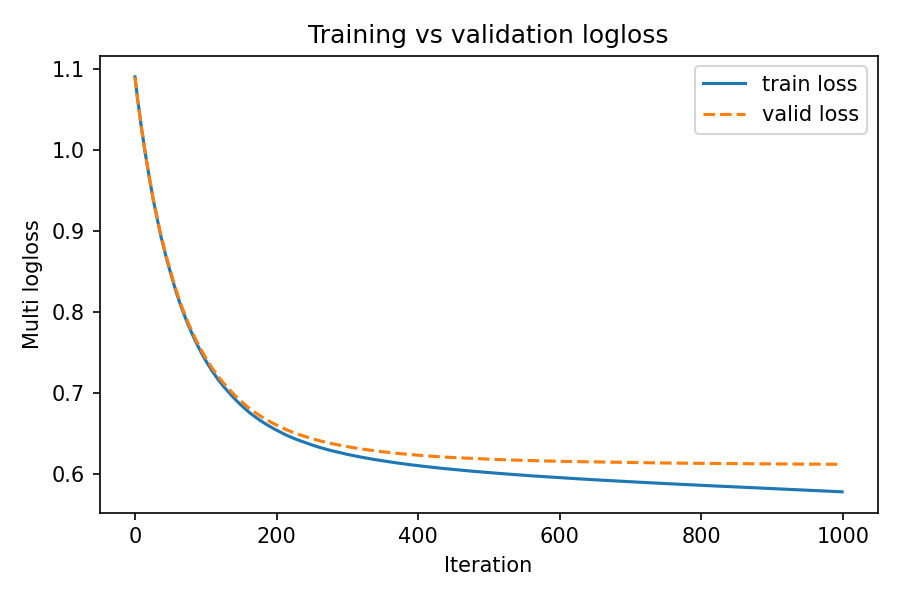
\includegraphics[width=0.50\linewidth]{Fig/training_curve_9.png}
  \caption{Évolution de la fonction de coût \textit{multi-logloss} sur les ensembles d’entraînement et de validation au cours de l’apprentissage LightGBM.}
  \label{fig:train-curve}
\end{figure}

\paragraph{Matrice de confusion.}

La matrice de confusion normalisée obtenue sur l’échantillon de test est représentée Figure~\ref{fig:cm}. Elle met en évidence des comportements sensiblement différents selon les espèces considérées et fournit une information plus riche que la seule accuracy globale.

\begin{itemize}
    \item \textbf{Pions $\pi^-$} : environ $48.8\,\%$ des événements sont correctement identifiés, tandis que $\sim47.9\,\%$ sont confondus avec des protons. La reconnaissance des pions constitue ainsi la principale difficulté du problème étudié.

    \item \textbf{Protons $p$} : la séparation est meilleure, avec $\sim68.6\,\%$ d’identifications correctes. L’erreur dominante correspond à une attribution erronée vers la classe pion ($\sim27.4\,\%$).

    \item \textbf{Kaons neutres $K^0_L$} : la classification est nettement plus performante, avec environ $86.0\,\%$ des événements correctement reconstruits, ce qui traduit une signature calorimétrique plus spécifique.
\end{itemize}

En supposant des classes de tailles comparables, ces résultats correspondent à une \textbf{accuracy globale} d’environ $68\,\%$. Cette valeur doit toutefois être interprétée avec prudence : elle traduit un niveau de performance global satisfaisant pour un problème hadronique multiclasse non trivial, mais masque des disparités importantes entre classes.

Le résultat le plus marquant n’est donc pas tant la valeur moyenne de l’accuracy que la structure des erreurs observées. La confusion massive entre pions et protons indique que ces deux espèces occupent des régions partiellement recouvrantes dans l’espace des variables utilisées, tandis que les $K^0_L$ se distinguent beaucoup plus nettement.

Cette dissymétrie justifie l’usage de métriques complémentaires telles que les rappels par classe, l’accuracy équilibrée ou les courbes ROC one-vs-rest, mieux adaptées pour caractériser finement les performances d’un classificateur multiclasse.

\begin{figure}[!ht]
  \centering
  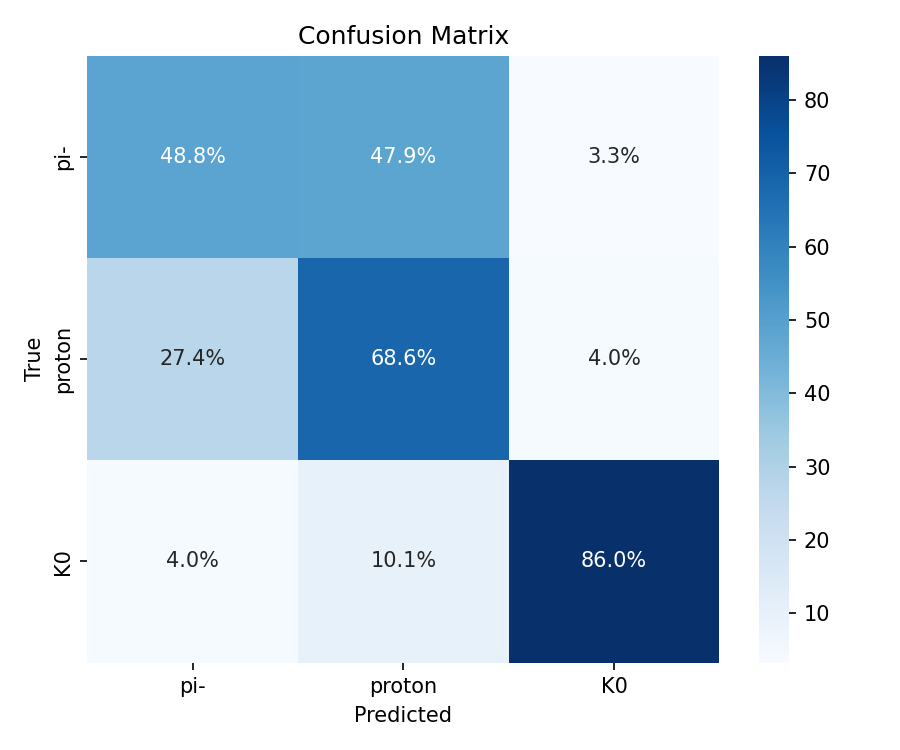
\includegraphics[width=0.50\linewidth]{Fig/confusion_matrix_9.png}
  \caption{Matrice de confusion normalisée (pourcentages par ligne). Les classes sont ordonnées selon \{$\pi^-$, $p$, $K^0_L$\}.}
  \label{fig:cm}
\end{figure}

\paragraph{Interprétation physique.}

La meilleure séparation observée pour les $K^0_L$ s’explique principalement par une dynamique hadronique différente de celle des pions et des protons, qui se répercute directement sur la morphologie des gerbes mesurées dans le SDHCAL.

Dans les interactions hadroniques se produisant dans l’absorbeur, les états finaux sont très souvent dominés par la production de pions. Ce comportement résulte conjointement :

\begin{itemize}
    \item de la faible masse des pions, qui les rend énergétiquement faciles à produire ;
    \item des symétries approximatives de l’interaction forte, notamment liées à l’isospin ;
    \item d’un espace de phase plus favorable ;
    \item de l’absence de création de quarks étranges supplémentaires.
\end{itemize}

À l’inverse, la production de kaons nécessite la création d’étrangeté (\(s\bar{s}\)) et implique des masses plus élevées. Elle est donc statistiquement moins probable aux énergies considérées ici. Les hadrons contenant de l’étrangeté, comme les $K^0_L$, présentent ainsi des modes d’interaction et des cascades secondaires en moyenne différents de ceux dominés par les pions.

Un rôle important est également joué par la production de mésons neutres $\pi^0$, qui se désintègrent quasi instantanément selon :

\[
\pi^0 \rightarrow \gamma\gamma.
\]

Ils alimentent alors la composante électromagnétique de la gerbe. Les fluctuations du nombre de $\pi^0$ produits influencent directement la compacité locale, la densité d’activité et le développement longitudinal observés dans le calorimètre. Les différences statistiques de production de ces composantes entre espèces contribuent donc au pouvoir discriminant du classificateur.

Les $K^0_L$ tendent ainsi à générer des signatures calorimétriques plus spécifiques, ce qui explique leur meilleure séparation expérimentale.

À l’inverse, les protons et les pions chargés présentent des comportements plus proches. Tous deux interagissent via l’interaction forte sans nécessiter de dynamique d’étrangeté, et leurs gerbes restent largement dominées par les fluctuations de première interaction nucléaire ainsi que par la variabilité de la composante électromagnétique secondaire. Il en résulte un recouvrement important dans l’espace des variables tabulaires utilisées ici, rendant leur frontière de séparation plus difficile à apprendre.

La confusion résiduelle pion/proton ne traduit donc pas une faiblesse particulière du modèle, mais reflète avant tout la proximité physique réelle de leurs signatures hadroniques dans le SDHCAL.

\paragraph{Probabilités prédites.}

Les histogrammes des probabilités de sortie du modèle (Figure~\ref{fig:hists}) confirment les tendances mises en évidence par la matrice de confusion et apportent une information complémentaire sur le degré de confiance des prédictions.

Les vrais $K^0_L$ reçoivent majoritairement des probabilités élevées pour leur classe correcte, avec une superposition limitée avec les distributions associées aux pions et aux protons. Cette séparation nette indique que le modèle identifie, pour une large fraction des événements, des signatures caractéristiques propres aux kaons neutres longs.

En revanche, les probabilités associées à la classe proton présentent un recouvrement significatif entre vrais protons et vrais pions. Une fraction non négligeable des événements des deux classes reçoit des scores intermédiaires, traduisant une zone d’ambiguïté où la décision du classificateur devient moins robuste.

Ce comportement est cohérent avec la proximité physique des signatures pion/proton dans le détecteur : pour certains événements, les observables de gerbe ne permettent pas une discrimination franche, même pour un modèle performant. La confusion observée ne provient donc pas uniquement de limites algorithmiques, mais également d’un recouvrement intrinsèque entre classes dans l’espace des variables utilisées.

Ces distributions suggèrent enfin qu’une exploitation probabiliste des sorties du modèle (seuils ajustés, calibration des scores, sélection d’événements de haute pureté) pourrait constituer une piste intéressante selon les besoins d’analyse.

\begin{figure}[!ht]
  \centering
  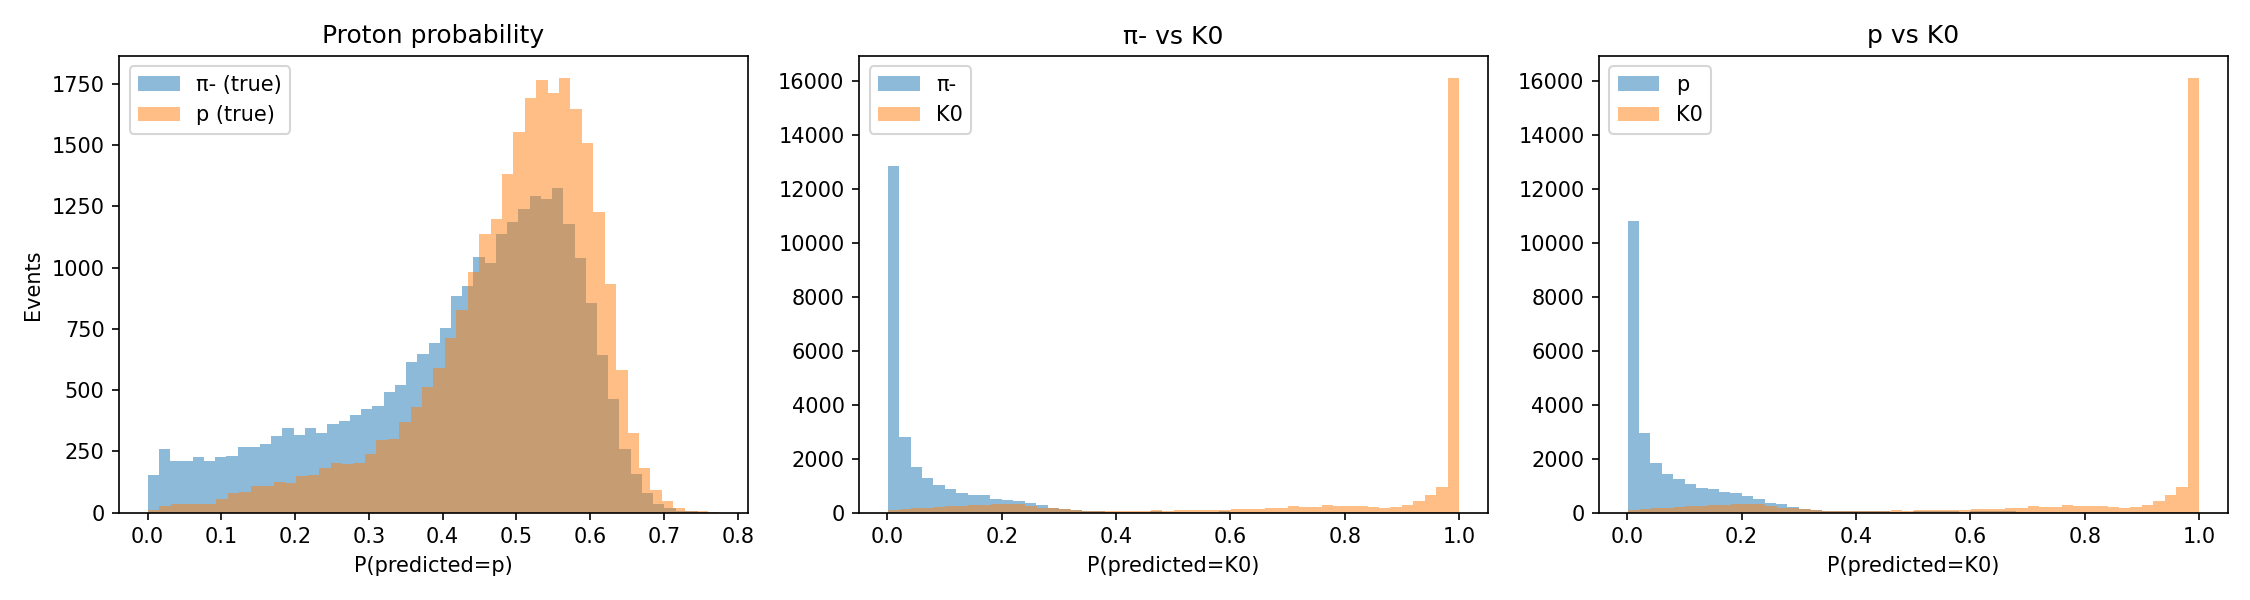
\includegraphics[width=\linewidth]{Fig/prob_hists_9.png}
  \caption{Histogrammes des probabilités prédites : (gauche) $P(\mathrm{classe}=p)$ pour vrais $\pi^-$ et vrais $p$ ; (centre) $P(\mathrm{classe}=K^0)$ pour vrais $\pi^-$ et vrais $K^0_L$ ; (droite) $P(\mathrm{classe}=K^0)$ pour vrais $p$ et vrais $K^0_L$.}
  \label{fig:hists}
\end{figure}

\paragraph{Bilan.}

Le classificateur LightGBM fournit ainsi une base solide pour l’identification hadronique tabulaire dans le SDHCAL. La séparation des $K^0_L$ apparaît robuste et bien maîtrisée, tandis que la confusion résiduelle entre protons et pions constitue la principale limitation actuelle du problème étudié.

L’accuracy globale d’environ $68\,\%$ doit ainsi être interprétée comme le résultat d’un compromis entre une excellente reconnaissance des $K^0_L$ et une séparation plus délicate du couple pion/proton, physiquement plus proche. Cette lecture détaillée est plus informative que la seule performance moyenne.

Ces observations motivent à la fois l’étude approfondie des variables discriminantes, l’usage de métriques par classe, ainsi que l’exploration de représentations plus fines des gerbes, notamment fondées directement sur les hits du détecteur.

\subsection{Corrélations et variables discriminantes}
\label{subsec:corr-perm}

Au-delà des performances globales du classificateur, il est important d’identifier quelles observables portent l’information la plus utile pour la séparation des particules. Cette analyse poursuit un double objectif : mieux comprendre les mécanismes physiques exploités par le modèle et repérer d’éventuelles redondances entre variables d’entrée.

Deux approches complémentaires ont été retenues :
\begin{itemize}
    \item l’étude des corrélations linéaires entre variables, à l’aide de la matrice de corrélation de Pearson ;
    \item l’analyse des importances internes du modèle LightGBM, estimées ici à partir du \emph{gain} cumulé apporté par chaque variable lors des coupures successives.
\end{itemize}

\paragraph{Matrice de corrélation.}

La Figure~\ref{fig:corr-matrix} présente la matrice de corrélation calculée sur l’ensemble des événements. Plusieurs groupes cohérents apparaissent naturellement.

\begin{itemize}
    \item \textbf{Activité globale et compacité de gerbe :} les variables \texttt{Thr1}, \texttt{Thr2}, \texttt{Thr3}, \texttt{NClusters}, \texttt{Nmax}, \texttt{AvgClustSize}, \texttt{MaxClustSize} et \texttt{Density} présentent des corrélations modérées à fortes. Cette structure est attendue, car ces observables mesurent toutes, sous des formes différentes, l’intensité locale ou globale de la gerbe.

    \item \textbf{Développement longitudinal :} \texttt{Begin}, \texttt{Zbary}, \texttt{Zrms}, \texttt{Xmax} et \texttt{z0\_fit} sont positivement corrélées. Elles décrivent conjointement la position de départ et l’évolution de la gerbe dans la profondeur du calorimètre.

    \item \textbf{Forme géométrique :} \texttt{\(\lambda_1\)}, \texttt{\(\lambda_2\)} et \texttt{eccentricity3D} apparaissent liées, ce qui reflète leur rôle commun dans la description de l’anisotropie spatiale.

    \item \textbf{Variables temporelles :} \texttt{tMin}, \texttt{tMean} et \texttt{tSpread} sont faiblement à modérément corrélées entre elles. Elles montrent également certains liens avec les variables longitudinales, suggérant une connexion entre chronologie du signal et profondeur d’initiation de la gerbe.
\end{itemize}

\begin{figure}[!ht]
  \centering
  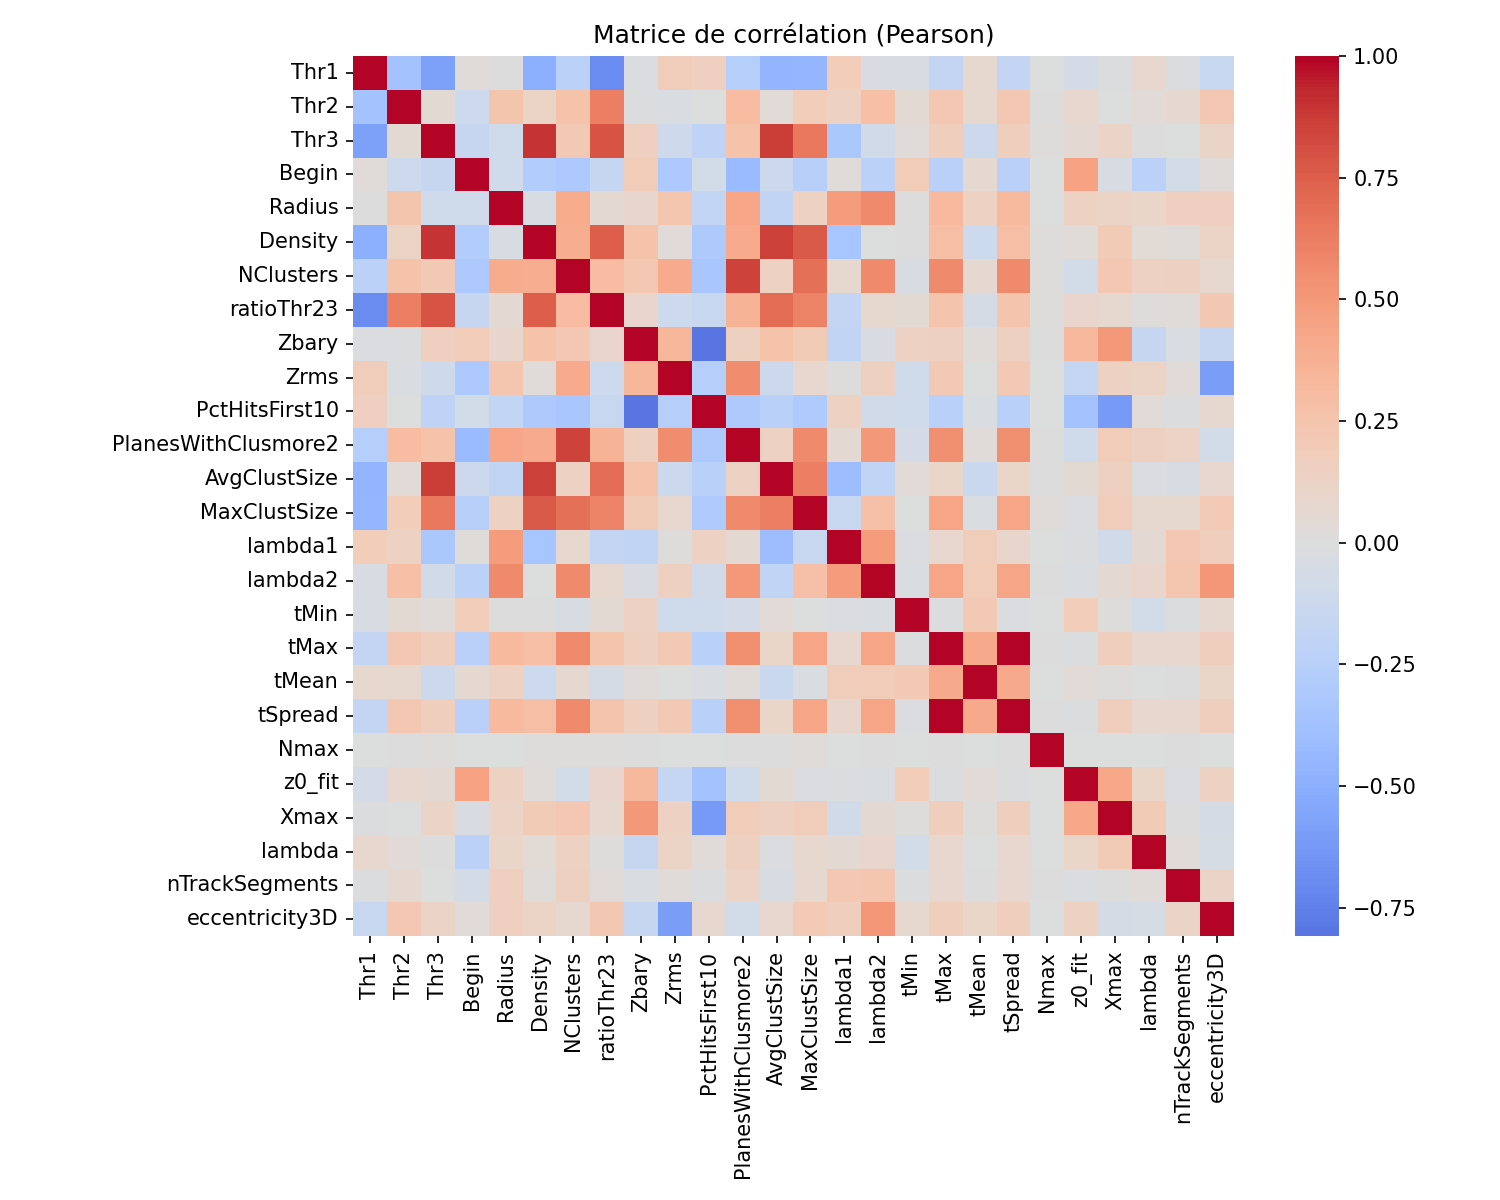
\includegraphics[width=0.75\linewidth]{Fig/correlation_matrix.png}
  \caption{Matrice de corrélation de Pearson des variables d’entrée utilisées pour la classification.}
  \label{fig:corr-matrix}
\end{figure}

Dans l’ensemble, cette organisation indique que plusieurs variables transportent une information partiellement redondante. Une sélection plus compacte des observables pourrait donc être envisagée sans perte majeure de performance.

\paragraph{Importances des variables dans LightGBM.}

La Figure~\ref{fig:perm-imp} présente les importances des variables estimées à partir du \emph{gain} cumulé de LightGBM. Cette quantité mesure la contribution totale de chaque variable à la réduction de la fonction de coût au cours de l’entraînement. Elle fournit ainsi une indication directe des observables les plus exploitées par le classificateur.

\begin{figure}[!ht]
  \centering
  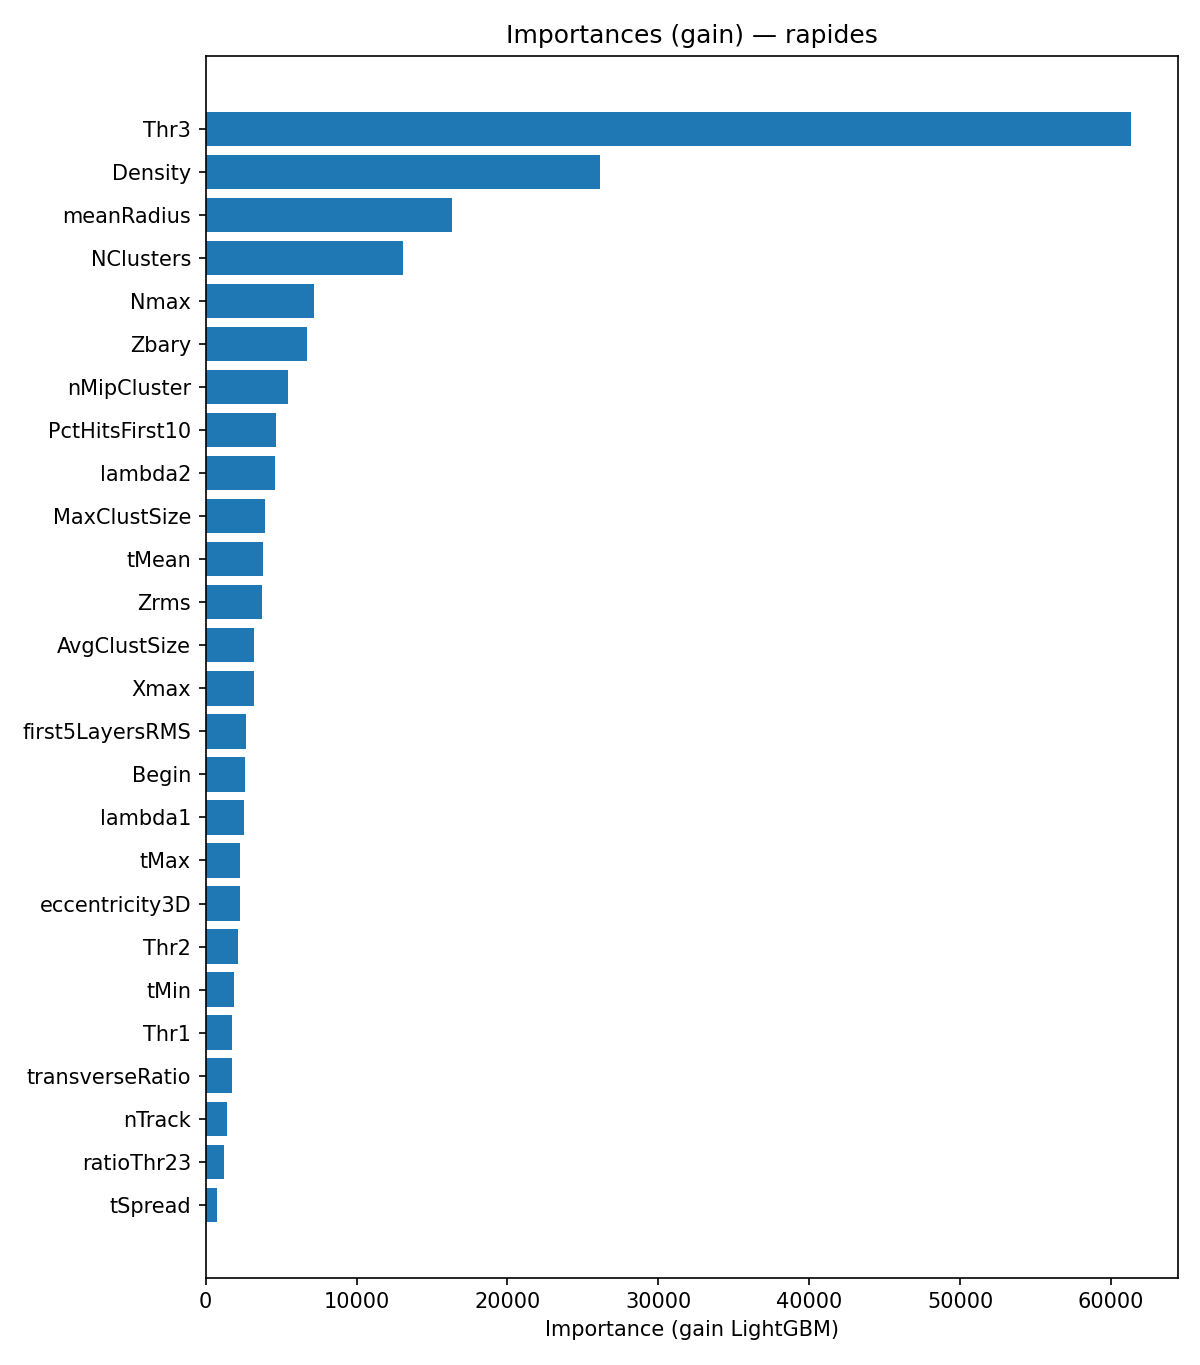
\includegraphics[width=0.90\linewidth,height=0.70\linewidth]{Fig/permutation_importances.png}
  \caption{Importances des variables extraites du modèle LightGBM à partir du gain cumulé.}
  \label{fig:perm-imp}
\end{figure}

\paragraph{Variables dominantes.}

La variable \texttt{Thr3}, correspondant au nombre de hits franchissant le seuil le plus élevé, apparaît comme la plus discriminante, nettement devant les autres. Ce résultat indique que les régions les plus denses de la gerbe jouent un rôle central dans la séparation des espèces. Il suggère que la structure des zones fortement actives constitue une signature importante de l’interaction hadronique.

Les variables \texttt{Density} et \texttt{meanRadius} figurent également parmi les contributions les plus élevées. Elles montrent que la compacité locale et l’extension transverse moyenne de la gerbe sont particulièrement informatives. Le classificateur semble donc s’appuyer fortement sur la morphologie spatiale de l’événement.

Un second groupe d’observables importantes regroupe \texttt{NClusters}, \texttt{Nmax}, \texttt{Zbary}, \texttt{nMipCluster} et \texttt{PctHitsFirst10}. Ces variables traduisent la fragmentation de l’activité, la multiplicité locale et le développement longitudinal de la gerbe, complétant l’information portée par les variables de densité et de compacité.

À l’inverse, les variables temporelles apparaissent ici à un rang plus secondaire. Dans cette configuration, le pouvoir discriminant du modèle est donc principalement porté par les observables décrivant l’intensité locale, la structure spatiale et le développement géométrique des gerbes, davantage que par leur chronologie.

\paragraph{Enseignements pour le PID.}

Cette analyse montre que la séparation des particules repose principalement sur trois familles d’information :
\begin{itemize}
    \item \textbf{la densité locale d’activité}, via \texttt{Thr3} et \texttt{Density} ;
    \item \textbf{la morphologie transverse}, via \texttt{meanRadius} ;
    \item \textbf{la structuration longitudinale et la fragmentation de la gerbe}, via \texttt{Zbary}, \texttt{NClusters} et \texttt{Nmax}.
\end{itemize}

Ces résultats sont cohérents avec la physique des gerbes hadroniques dans un calorimètre hautement granulaire : la compacité, la multiplicité secondaire et la répartition spatiale de l’activité constituent des signatures plus robustes que les seules variables temporelles.

\paragraph{Conséquences pratiques.}

Ces observations suggèrent plusieurs pistes d’amélioration :
\begin{itemize}
    \item réaliser des études d’ablation par groupes de variables (densité, longitudinal, transverse, temps) ;
    \item simplifier le jeu d’entrée en supprimant certaines variables redondantes ;
    \item approfondir l’interprétabilité du modèle à l’aide de méthodes locales telles que SHAP ;
    \item tester explicitement l’impact du retrait complet des variables temporelles.
\end{itemize}

\subsection{Discussion, robustesse et perspectives d'amélioration}

Les résultats obtenus montrent que l’approche par arbres de décision boostés constitue une base solide pour l’identification hadronique dans le SDHCAL. Les performances globales sont satisfaisantes, avec une séparation particulièrement nette des kaons neutres $K^0_L$, tandis que la confusion résiduelle entre protons $p$ et pions $\pi^-$ demeure la principale limitation du classificateur.

L’accuracy globale d’environ $68\,\%$ doit ainsi être interprétée comme un résultat encourageant pour un problème hadronique multiclasse non trivial, mais non comme une performance uniforme sur l’ensemble des classes. L’analyse détaillée par espèce reste donc indispensable.

\paragraph{Interprétation des performances observées.}

La bonne reconnaissance des $K^0_L$ est cohérente avec leur dynamique hadronique spécifique. La présence d’étrangeté, des canaux d’interaction distincts ainsi qu’une production secondaire différente de celle des pions et des protons peuvent modifier la fraction électromagnétique, la compacité locale ou encore le développement longitudinal de la gerbe.

À l’inverse, protons et pions chargés présentent des signatures plus proches. Tous deux interagissent fortement dans l’absorbeur et peuvent produire des cascades secondaires similaires, en particulier lorsque les fluctuations de première interaction dominent. Cette proximité physique se traduit directement par le recouvrement observé dans les distributions de probabilités prédites.

Il est également probable que cette difficulté de séparation dépende de l’énergie incidente : à basse énergie, la faible multiplicité de hits accentue les fluctuations statistiques, tandis qu’à plus haute énergie certaines signatures morphologiques deviennent plus marquées. Une étude différentielle par tranches d’énergie constituerait donc un prolongement naturel.

\paragraph{Robustesse vis-à-vis des effets instrumentaux.}

L’analyse des importances montre que les variables les plus utiles au modèle sont principalement liées à l’activité au seuil élevé, à la densité locale et à la géométrie de la gerbe. Cette hiérarchie apparaît physiquement plausible, mais doit être confirmée dans des conditions instrumentales réalistes.

Il sera notamment nécessaire d’évaluer la stabilité des performances en présence :

\begin{itemize}
    \item d’une résolution temporelle dégradée ;
    \item d’offsets de calibration entre couches ;
    \item de variations des conditions de prise de données ;
    \item d’inefficacités locales ou d’un bruit électronique résiduel ;
    \item de canaux défectueux ou instables.
\end{itemize}

De telles études permettraient de quantifier la sensibilité réelle du classificateur aux non-idéalités expérimentales et de mieux estimer sa transférabilité vers des données réelles.

\paragraph{Réduction et sélection de variables.}

La matrice de corrélation a montré que plusieurs observables transportent une information partiellement redondante, notamment au sein des variables décrivant l’activité globale et la compacité de la gerbe.

Une stratégie raisonnée de sélection de variables pourrait ainsi :

\begin{itemize}
    \item réduire la dimension du problème ;
    \item accélérer l’entraînement ;
    \item limiter la variance statistique ;
    \item améliorer l’interprétabilité physique du modèle.
\end{itemize}

Par exemple, conserver un représentant robuste par groupe corrélé (\texttt{Thr3} ou \texttt{Nmax}, \texttt{Density} ou \texttt{NClusters}, etc.) pourrait suffire sans perte notable de performance.

\paragraph{Améliorations possibles du modèle.}

Bien que LightGBM fournisse déjà de bons résultats, plusieurs axes d’optimisation restent envisageables :

\begin{itemize}
    \item ajustement fin des hyperparamètres (profondeur des arbres, taux d’apprentissage, régularisation L1/L2) ;
    \item pondération spécifique des classes ou des erreurs de classification ;
    \item calibration des probabilités de sortie (Platt scaling, isotonic regression) ;
    \item entraînement conditionné par tranches d’énergie ;
    \item validation croisée sur plusieurs découpages statistiques ;
    \item optimisation directe de métriques équilibrées plutôt que de la seule accuracy.
\end{itemize}

Un apprentissage par intervalles d’énergie pourrait être particulièrement pertinent, les signatures hadroniques évoluant sensiblement entre basse et haute énergie.

Des tests exploratoires de rééquilibrage des classes, notamment via SMOTE, peuvent également être envisagés. Néanmoins, l’intérêt réel de telles méthodes devra être mis en balance avec le risque d’introduire des événements synthétiques peu représentatifs de la physique simulée.

\paragraph{Systématiques liées à la simulation.}

Comme toute approche supervisée entraînée sur simulation, les performances mesurées dépendent du réalisme du modèle physique utilisé pour générer les gerbes hadroniques. Il conviendra donc d’évaluer l’impact :

\begin{itemize}
    \item du choix de la liste de physique utilisée dans Geant4 ;
    \item des paramètres de réponse du détecteur ;
    \item des inefficacités instrumentales ;
    \item de la modélisation temporelle des signaux ;
    \item d’éventuels écarts simulation / données réelles.
\end{itemize}

Une comparaison entre plusieurs configurations de simulation, ainsi qu’une confrontation future aux données expérimentales, permettrait d’estimer l’incertitude systématique associée au classificateur.

\paragraph{Vers des représentations plus fines.}

La principale limite de l’approche actuelle provient de l’utilisation d’un ensemble de variables agrégées. Bien que physiquement motivés, ces descripteurs ne restituent qu’une partie de la richesse spatiale et temporelle des hits bruts du détecteur.

Cela motive naturellement l’exploration de méthodes capables d’exploiter directement la structure native des événements, telles que :

\begin{itemize}
    \item les réseaux convolutifs 3D appliqués à une voxelisation des gerbes ;
    \item les réseaux de neurones graphiques (GNN) construits sur les graphes de hits ;
    \item des approches hybrides combinant descripteurs physiques et représentation brute.
\end{itemize}

\paragraph{Conclusion.}

Le classificateur LightGBM constitue ainsi une solution performante, rapide et interprétable pour l’identification hadronique tabulaire dans le SDHCAL. Ses principales limites actuelles proviennent moins de l’algorithme lui-même que du recouvrement physique entre certaines espèces, en particulier entre pions et protons.

Les progrès futurs passeront principalement par une meilleure maîtrise des effets instrumentaux, une validation approfondie sur conditions réalistes, des études différentielles en énergie et une exploitation plus directe de l’information spatio-temporelle complète des gerbes.

\section{Étude exploratoire : approche GNN}

\paragraph{Motivation.}

L’approche développée jusqu’à présent repose sur un ensemble de descripteurs globaux extraits à partir des hits du détecteur. Cette stratégie fournit une représentation compacte, physiquement interprétable et bien adaptée aux méthodes tabulaires. Elle ne conserve toutefois qu’une partie de l’information spatiale et temporelle contenue dans la topologie fine des gerbes hadroniques.

Or, le SDHCAL est un détecteur hautement granulaire, dont l’un des principaux atouts réside précisément dans la distribution détaillée des hits, couche par couche. Il est donc naturel d’explorer des méthodes capables d’exploiter directement cette information native, sans étape intermédiaire de réduction en variables agrégées.

Dans cette perspective, une étude exploratoire a été menée à l’aide de réseaux de neurones graphiques (\emph{Graph Neural Networks}, GNN).

\paragraph{Principe général.}

Un GNN représente chaque événement sous la forme d’un graphe :

\begin{itemize}
    \item les \textbf{nœuds} correspondent aux hits enregistrés dans le détecteur ;
    \item les \textbf{arêtes} relient des hits voisins ou compatibles selon des critères géométriques et temporels ;
    \item les \textbf{attributs des nœuds} peuvent inclure la position spatiale, le seuil franchi ou le temps associé au hit.
\end{itemize}

Le réseau apprend ensuite à propager et agréger localement l’information entre nœuds connectés afin de construire une représentation globale de la gerbe. Cette approche est particulièrement adaptée aux structures irrégulières, non cartésiennes et peu denses, typiques des calorimètres granulaires.

\paragraph{Cadre de l’étude réalisée.}

Dans le cadre de ce travail, cette méthode a été appliquée à une tâche ciblée de séparation binaire entre pions $\pi$ et protons $p$, sur des événements simulés entre 1 et 100~GeV. Les détails complets de la construction des graphes, du prétraitement des données et de l’architecture utilisée sont présentés en Annexe~\ref{app:gnn}.

Les résultats obtenus doivent être considérés comme préliminaires. Cette étude a été menée en fin de stage et n’a pas donné lieu à une campagne complète de validation systématique ni à l’ensemble des figures de synthèse disponibles pour les approches principales. Elle est donc présentée ici comme une preuve de concept destinée à évaluer le potentiel de cette famille de méthodes.

\paragraph{Résultats obtenus.}

Les premières observations mettent en évidence un rôle déterminant de l’information temporelle.

Lorsque les temps des hits sont conservés avec une précision quasi idéale issue de la simulation (résolution de l’ordre de $\sim10^{-6}$~ns), l’accuracy peut atteindre environ $90\,\%$. Une telle performance traduit principalement l’exploitation d’une information temporelle extrêmement discriminante, liée notamment aux différences de temps de vol entre pions et protons.

Il est important de noter qu’un comportement analogue est observé avec l’approche tabulaire fondée sur BDT lorsque le smearing appliqué à \texttt{tMin} est supprimé. Des performances du même ordre peuvent alors être obtenues. Cela indique que le gain observé provient en grande partie du caractère idéalisé de l’information temporelle disponible en simulation, plutôt que d’une supériorité intrinsèque du GNN sur ce problème de PID.

En revanche, lorsque la résolution temporelle est ramenée à une valeur plus réaliste, de l’ordre de $\sim10$~ps, la performance du GNN redescend autour de $60\,\%$, soit un niveau comparable à celui obtenu avec les méthodes tabulaires classiques.

Dans la configuration étudiée ici, aucun avantage net du GNN n’apparaît donc pour l’identification pion/proton en conditions réalistes.

\paragraph{Interprétation physique.}

La séparation proton/pion repose en partie sur la différence de masse entre les deux particules. À impulsion comparable, celle-ci se traduit par des temps de vol distincts, plus facilement exploitables lorsque la résolution temporelle devient extrêmement fine. Les excellentes performances observées sans smearing reflètent donc principalement l’accès à une information temporelle idéale, difficilement atteignable expérimentalement.

Par ailleurs, la structure locale des premières interactions hadroniques peut également différer subtilement entre les deux espèces. Un GNN est théoriquement capable de capter ce type de corrélations fines entre hits voisins, parfois peu visibles à travers des descripteurs globaux. Néanmoins, dans le cadre présent, cet avantage structurel ne se traduit pas encore par un gain clair dès lors que l’on adopte des conditions temporelles réalistes.

\paragraph{Limites actuelles.}

Cette approche présente plusieurs contraintes :

\begin{itemize}
    \item coût d’entraînement plus élevé que les méthodes tabulaires ;
    \item sensibilité accrue au choix des hyperparamètres ;
    \item besoin de jeux de données volumineux ;
    \item interprétabilité plus limitée ;
    \item dépendance marquée à la définition du graphe (voisinage, connectivité).
\end{itemize}

Dans le cadre présent, il s’agit donc davantage d’une étude exploratoire que d’une alternative immédiatement opérationnelle aux méthodes de boosting.

\paragraph{Perspectives.}

Même si le GNN ne semble pas apporter ici d’amélioration décisive pour le PID, il demeure une approche très prometteuse pour d’autres tâches où la structure détaillée des gerbes joue un rôle plus direct.

En particulier, il paraît potentiellement mieux adapté à la \textbf{reconstruction de l’énergie}, pour laquelle l’exploitation fine de la topologie complète des hits, de leurs corrélations spatiales et de leur organisation locale pourrait fournir un avantage plus marqué que dans une simple classification binaire.

Les GNN pourraient ainsi être particulièrement utiles pour :

\begin{itemize}
    \item la reconstruction d’énergie à partir de la structure complète de la gerbe ;
    \item la reconstruction simultanée PID + énergie ;
    \item les approches de type \emph{Particle Flow} ;
    \item la séparation de gerbes chevauchantes ;
    \item l’exploitation conjointe des informations spatiales et temporelles.
\end{itemize}

Des variantes plus avancées, fondées sur des mécanismes d’attention ou sur l’apprentissage différentiable de la connectivité, pourraient également améliorer les performances futures.

\paragraph{Bilan.}

Cette étude exploratoire montre que les réseaux de neurones graphiques constituent une voie crédible pour exploiter pleinement le potentiel du SDHCAL. Toutefois, dans le cas particulier du PID pion/proton étudié ici, les résultats actuels n’indiquent pas d’avantage clair par rapport au BDT lorsque l’on adopte des conditions temporelles réalistes. En revanche, leur capacité à exploiter directement la structure détaillée des hits en fait une piste particulièrement intéressante pour de futurs travaux consacrés à la reconstruction de l’énergie.


\section{Synthèse}

Ce chapitre a présenté une étude d’identification hadronique dans le SDHCAL fondée sur des méthodes d’apprentissage supervisé appliquées à des échantillons simulés de pions négatifs $\pi^-$, de protons $p$ et de kaons neutres longs $K^0_L$. L’objectif était d’exploiter la richesse spatiale, semi-digitale et géométrique du détecteur afin de distinguer automatiquement ces différentes espèces à partir de la topologie de leurs gerbes.

Parmi les approches testées, les arbres de décision boostés, implémentés via LightGBM, ont offert le meilleur compromis entre performance, rapidité d’entraînement et interprétabilité. Les résultats obtenus sur l’échantillon de test conduisent à une \textbf{accuracy globale d’environ $68\,\%$}. Cette valeur traduit un niveau de performance satisfaisant pour un problème hadronique multiclasse non trivial, mais masque des contrastes importants entre espèces : la séparation des $K^0_L$ apparaît robuste, tandis que la confusion résiduelle entre protons et pions constitue la principale limite actuelle du classificateur.

L’analyse des corrélations entre variables et des importances internes du modèle a permis d’identifier les observables les plus discriminantes. Les variables associées à la densité locale d’activité, au franchissement du seuil élevé (\texttt{Thr3}), à la compacité de la gerbe (\texttt{Density}) ainsi qu’à son extension transverse (\texttt{meanRadius}) apparaissent comme les contributions dominantes. Ce constat est cohérent avec la physique des interactions hadroniques, où la structuration spatiale et l’intensité locale des dépôts constituent des signatures particulièrement informatives.

Ces résultats montrent que le SDHCAL possède un réel potentiel pour l’identification hadronique, y compris dans le cadre d’approches tabulaires relativement simples. Ils soulignent plus largement l’intérêt des calorimètres hautement granulaires, capables de restituer finement la morphologie des gerbes et d’alimenter des méthodes d’analyse avancées.

Ils indiquent également que les limites actuelles proviennent autant de la proximité physique réelle entre certaines espèces hadroniques que du choix de l’algorithme lui-même. Dans le cas pion/proton, le recouvrement partiel des signatures de gerbe rend la séparation intrinsèquement plus délicate.

En parallèle, l’exploration préliminaire d’une approche par réseaux de neurones graphiques a confirmé l’intérêt des représentations construites directement à partir des hits du détecteur. Si aucun gain net n’a été mis en évidence ici pour le PID dans des conditions réalistes, ces méthodes apparaissent comme une piste prometteuse pour exploiter plus complètement la connectivité spatiale des événements, notamment en vue de la reconstruction de l’énergie.

L’ensemble de ces travaux constitue ainsi une base solide pour la suite de ce mémoire, consacrée à un second enjeu majeur de la calorimétrie hadronique : la reconstruction précise de l’énergie incidente.


\chapter{Reconstruction de l'énergie}
\label{sec:energy_reco}

\section{Enjeux de la reconstruction d’énergie dans le SDHCAL}
\label{subsec:energy_challenges}

La mesure de l’énergie des particules hadroniques constitue l’un des objectifs centraux d’un calorimètre hadronique. Dans un détecteur tel que le SDHCAL, cette tâche est rendue possible par l’enregistrement détaillé du développement spatial de la gerbe dans les couches successives du détecteur. Toutefois, contrairement au cas électromagnétique, la reconstruction de l’énergie hadronique demeure intrinsèquement plus délicate en raison de la complexité des interactions nucléaires mises en jeu.

Une gerbe hadronique présente en effet d’importantes fluctuations événement par événement. La profondeur de première interaction, la multiplicité des particules secondaires, la fraction électromagnétique de la gerbe, les pertes d’énergie invisibles liées aux processus nucléaires, ainsi que les fuites longitudinales ou latérales peuvent varier fortement pour une même énergie incidente. Ces effets dégradent à la fois la linéarité de la réponse et la résolution énergétique, et rendent difficile l’établissement d’une relation simple entre l’énergie vraie de la particule et les observables enregistrées dans le calorimètre.

Dans le cas du SDHCAL, la situation présente à la fois des limitations et des opportunités. D’un côté, la lecture semi-digitale ne mesure pas directement une énergie déposée continue, mais seulement le franchissement de trois seuils de charge. La réponse du détecteur est donc sensible aux effets de saturation locale dans les zones les plus denses de la gerbe, ainsi qu’à la non-compensation intrinsèque du calorimètre. D’un autre côté, la très forte granularité du détecteur fournit un accès détaillé à la morphologie des gerbes, à leur compacité, à leur développement longitudinal et à leur structure locale. Cette richesse d’information ouvre la possibilité de dépasser une simple reconstruction fondée sur le nombre total de hits.

Deux approches complémentaires peuvent alors être envisagées. La première consiste à utiliser une méthode paramétrique fondée sur les nombres de hits enregistrés aux différents seuils, avec des coefficients ajustés de manière à reproduire au mieux l’énergie incidente. Cette stratégie reste proche des méthodes classiques de calibration calorimétrique et conserve une bonne interprétabilité physique. La seconde repose sur des techniques d’apprentissage supervisé, capables d’exploiter simultanément un grand nombre d’observables décrivant la gerbe, et donc de capturer des dépendances non linéaires plus complexes entre la topologie de l’événement et l’énergie vraie.

Dans ce chapitre, nous comparons ces deux stratégies de reconstruction dans le SDHCAL. Nous étudions d’abord une méthode analytique par comptage de seuils, calibrée par minimisation du $\chi^2$, puis une approche de régression par arbres de décision boostés. L’objectif est d’évaluer dans quelle mesure l’enrichissement des observables et l’usage de méthodes d’apprentissage permettent d’améliorer la linéarité et la résolution énergétique.

L’étude se concentre principalement sur les pions et les protons. Les kaons neutres longs ont surtout été considérés, dans la partie PID, comme une classe de contrôle dont l’identification est relativement aisée. La reconstruction d’énergie présentée ici porte donc en priorité sur les espèces pour lesquelles l’enjeu méthodologique est le plus significatif, en particulier dans une chaîne d’analyse combinant identification et estimation d’énergie.

\section{Jeux de données et protocole d’évaluation}
\label{subsec:Data_protocol}

L’étude de reconstruction d’énergie présentée dans ce chapitre repose sur des échantillons simulés de pions négatifs \(\pi^-\) et de protons \(p\), qui constituent les deux espèces les plus pertinentes pour l’évaluation des performances énergétiques dans la chaîne d’analyse considérée. Les kaons neutres longs, déjà étudiés dans la partie identification, ne sont pas inclus ici, l’objectif étant de concentrer l’analyse sur les cas les plus exigeants du point de vue de la reconstruction.

\subsection*{Échantillon d’apprentissage}

Un jeu principal d’environ \(2\times10^5\) événements est utilisé pour l’apprentissage des modèles. Les énergies incidentes y sont réparties uniformément entre \SI{1}{GeV} et \SI{130}{GeV}, ce qui permet d’exposer les algorithmes à l’ensemble du domaine énergétique étudié. Cette distribution continue favorise l’apprentissage d’une réponse globale valable aussi bien aux basses qu’aux hautes énergies.

Pour les méthodes d’apprentissage supervisé, cet échantillon est subdivisé selon un schéma classique :

\begin{itemize}
    \item \(70\,\%\) des événements pour l’entraînement ;
    \item \(15\,\%\) pour la validation interne, utilisée pour le suivi de l’apprentissage, l’arrêt anticipé et le réglage des hyperparamètres ;
    \item \(15\,\%\) conservés comme sous-échantillon indépendant.
\end{itemize}

Cette séparation intervient uniquement dans la phase d’optimisation interne des modèles de type LightGBM.

\subsection*{Échantillon d’évaluation physique}

Afin d’obtenir des performances lisibles et directement comparables en fonction de l’énergie, les résultats reportés dans ce mémoire sont évalués sur un second jeu de données indépendant, construit spécifiquement pour l’analyse physique.

Cet échantillon contient \textbf{10\,000 événements par point d’énergie}, pour des valeurs discrètes :

\[
5,\ 10,\ 15,\ \dots,\ 100~\text{GeV}.
\]

Il s’agit donc d’un ensemble régulier, à statistique homogène, particulièrement adapté à l’étude de la linéarité et de la résolution calorimétrique.

Dans la suite du chapitre, ce jeu constitue la référence commune utilisée pour comparer les différentes méthodes de reconstruction, qu’il s’agisse :

\begin{itemize}
    \item de la méthode paramétrique par minimisation du \(\chi^2\) ;
    \item de la régression par arbres de décision boostés ;
    \item ou des comparaisons globales entre approches.
\end{itemize}

\subsection*{Observables de performance}

Les performances de reconstruction sont étudiées dans chaque bin d’énergie à l’aide de plusieurs indicateurs complémentaires.

\paragraph{Linéarité.}

Pour chaque énergie incidente \(E_{\mathrm{true}}\), on calcule la moyenne de l’énergie reconstruite :

\[
\langle E_{\mathrm{reco}} \rangle.
\]

Une réponse idéale correspond à :

\[
\langle E_{\mathrm{reco}} \rangle = E_{\mathrm{true}}.
\]

Les écarts à cette diagonale traduisent un défaut de calibration ou une non-linéarité résiduelle.

\paragraph{Biais relatif.}

Le biais est quantifié par :

\[
\delta(E)=
\frac{\langle E_{\mathrm{reco}}\rangle-E_{\mathrm{true}}}{E_{\mathrm{true}}}.
\]

Une valeur positive indique une surestimation systématique, tandis qu’une valeur négative traduit une sous-réponse.

\paragraph{Résolution énergétique.}

Pour chaque énergie, la distribution des résidus est ajustée par une loi gaussienne. La largeur extraite du fit, notée \(\sigma(E)\), permet de définir la résolution relative :

\[
\frac{\sigma(E)}{E}.
\]

Cette grandeur mesure la précision événement par événement de la reconstruction.

\subsection*{Intérêt du protocole}

L’utilisation d’un échantillon indépendant, équilibré en énergie et statistiquement homogène, permet une comparaison robuste des méthodes. Elle évite également qu’une surreprésentation de certaines énergies dans l’échantillon d’apprentissage n’influence artificiellement les performances reportées.

Ce protocole est particulièrement bien adapté à une étude calorimétrique, où la qualité de reconstruction dépend fortement de l’énergie incidente. Il permet d’identifier clairement les domaines d’énergie où chaque méthode est la plus performante, ainsi que les éventuelles limitations observées aux basses et hautes énergies.


\section{Méthode paramétrique par comptage de seuils}
\label{subsec:parametric_chi2}

Avant d’introduire des approches d’apprentissage automatique plus complexes, il est naturel de considérer une méthode de reconstruction fondée directement sur la physique de la réponse du détecteur. Dans le cas du SDHCAL, la lecture semi-digitale fournit, pour chaque cellule active, non pas une énergie déposée continue, mais l’information du franchissement de trois seuils de charge croissants. La reconstruction de l’énergie incidente doit donc être déduite de la distribution des hits entre ces différents niveaux de seuil.

\subsection*{Principe général}

Pour chaque événement, on définit :

\begin{itemize}
    \item $N_1$ : nombre de hits ayant franchi uniquement le premier seuil ;
    \item $N_2$ : nombre de hits associés au second seuil ;
    \item $N_3$ : nombre de hits associés au troisième seuil ;
\end{itemize}

ainsi que le nombre total de hits :

\[
N_{\mathrm{hit}} = N_1 + N_2 + N_3.
\]

Ces trois multiplicit\'es contiennent une information indirecte sur la quantit\'e d'\'energie d\'epos\'ee dans le calorim\`etre. En premi\`ere approximation :
\begin{itemize}
    \item les hits de seuil bas sont nombreux dans les régions peu ionisantes ;
    \item les hits de seuil élevé apparaissent préférentiellement dans les zones denses de la gerbe ;
    \item la répartition entre seuils reflète donc la structure locale du dépôt d’énergie.
\end{itemize}

Il est alors possible de construire une estimation de l’énergie incidente comme une combinaison pondérée des trois compteurs.

\subsection*{Formulation de la reconstruction}

L’énergie reconstruite est écrite sous la forme :

\[
E_{\mathrm{reco}}
=
\alpha(N_{\mathrm{hit}})\,N_1
+
\beta(N_{\mathrm{hit}})\,N_2
+
\gamma(N_{\mathrm{hit}})\,N_3,
\]

où $\alpha$, $\beta$ et $\gamma$ sont des coefficients effectifs dépendant du nombre total de hits.

Cette dépendance en $N_{\mathrm{hit}}$ est introduite afin de prendre en compte le fait que la réponse du calorimètre n’est pas strictement linéaire sur toute la gamme d’énergie. En particulier :

\begin{itemize}
    \item à basse énergie, les fluctuations statistiques dominent ;
    \item à haute énergie, des effets de saturation locale apparaissent ;
    \item la composition relative de la gerbe évolue avec l’énergie incidente.
\end{itemize}

Pour absorber ces effets, les coefficients sont paramétrés par des fonctions polynomiales de faible degré :

\[
\alpha(N_{\mathrm{hit}})=a_0+a_1N_{\mathrm{hit}}+a_2N_{\mathrm{hit}}^2,
\]

\[
\beta(N_{\mathrm{hit}})=b_0+b_1N_{\mathrm{hit}}+b_2N_{\mathrm{hit}}^2,
\]

\[
\gamma(N_{\mathrm{hit}})=c_0+c_1N_{\mathrm{hit}}+c_2N_{\mathrm{hit}}^2.
\]

Les neuf coefficients libres $(a_i,b_i,c_i)$ sont ensuite déterminés à partir des données simulées.

\subsection*{Motivation physique}

Cette méthode repose sur plusieurs idées simples :

\begin{itemize}
    \item le nombre total de hits croît globalement avec l’énergie incidente ;
    \item les seuils élevés transportent une information supplémentaire sur les zones très denses de la gerbe ;
    \item une pondération distincte des trois seuils permet de corriger partiellement les effets de non-linéarité du détecteur ;
    \item la dépendance en $N_{\mathrm{hit}}$ agit comme une calibration dynamique selon le régime énergétique.
\end{itemize}

Ainsi, bien qu’elle reste analytique et relativement simple, cette approche exploite déjà une partie importante de l’information spécifique au SDHCAL.

\subsection*{Intérêt et limites}

Cette stratégie présente plusieurs avantages :

\begin{itemize}
    \item interprétation physique directe ;
    \item nombre réduit de paramètres ;
    \item mise en œuvre rapide ;
    \item robustesse statistique ;
    \item référence naturelle pour comparer des méthodes plus avancées.
\end{itemize}

Elle reste toutefois limitée par sa forme fonctionnelle imposée. Les corrélations complexes entre variables, la topologie détaillée des gerbes ou certaines non-linéarités fines du détecteur ne peuvent être décrites que partiellement dans ce cadre paramétrique.

Pour cette raison, cette méthode constitue à la fois un outil de reconstruction performant et un point de comparaison essentiel avant l’introduction d’approches basées sur l’apprentissage supervisé.

%%%%%%%%%%%%%%

\section{Ajustement des paramètres par minimisation du \texorpdfstring{$\chi^2$}{chi²}}

Les coefficients intervenant dans la paramétrisation de l’énergie reconstruite ne sont pas fixés a priori. Ils doivent être déterminés à partir d’un échantillon de référence pour lequel l’énergie incidente vraie est connue. Dans cette étude, cette calibration est réalisée sur les données simulées en ajustant les paramètres de manière à minimiser l’écart entre l’énergie reconstruite et l’énergie générée.
Dans cette étude, la calibration paramétrique est réalisée séparément pour chaque espèce hadronique considérée. Un jeu de coefficients spécifique est donc ajusté pour les pions négatifs $\pi^-$ et un autre pour les protons $p$, afin de tenir compte des différences de développement des gerbes et de réponse calorimétrique entre espèces.

\subsection*{Fonction objectif}

Pour chaque événement $i$, on dispose :

\begin{itemize}
    \item de l’énergie vraie $E_i^{\mathrm{true}}$ imposée par la simulation ;
    \item des observables $(N_1,N_2,N_3)_i$ mesurées dans le calorimètre ;
    \item d’une énergie reconstruite $E_i^{\mathrm{reco}}(\vec{\theta})$ dépendant du vecteur de paramètres
    \[
    \vec{\theta}=(a_0,a_1,a_2,\; b_0,b_1,b_2,\; c_0,c_1,c_2).
    \]
\end{itemize}

Les paramètres sont obtenus en minimisant la quantité :

\[
\chi^2(\vec{\theta})
=
\sum_{i=1}^{N}
\left(
\frac{E_i^{\mathrm{reco}}(\vec{\theta})-E_i^{\mathrm{true}}}
{\sigma_i}
\right)^2,
\]

où $\sigma_i$ représente une incertitude effective associée à l’événement ou au bin d’énergie considéré.

Dans la pratique, cette minimisation revient à rechercher la combinaison de coefficients donnant la meilleure concordance moyenne entre énergie reconstruite et énergie vraie sur l’ensemble de calibration.

\subsection*{Choix du domaine d’ajustement}

L’ajustement est réalisé sur l’ensemble continu d’entraînement couvrant uniformément la gamme :

\[
1 \leq E_{\mathrm{true}} \leq 130~\mathrm{GeV}.
\]

Ce choix présente plusieurs avantages :

\begin{itemize}
    \item contraindre la calibration sur toute la dynamique accessible ;
    \item limiter les extrapolations aux hautes énergies ;
    \item lisser les fluctuations statistiques locales ;
    \item obtenir des coefficients utilisables sur un large domaine.
\end{itemize}

Les performances finales sont ensuite évaluées sur un échantillon indépendant constitué de points discrets tous les 5 GeV, ce qui permet une lecture claire de la linéarité et de la résolution.

\subsection*{Outil de minimisation}

La minimisation numérique est effectuée à l’aide de \texttt{Minuit}, largement utilisé en physique des particules pour les ajustements multi-paramètres. Cet outil permet :

\begin{itemize}
    \item la recherche efficace du minimum global ;
    \item l’estimation des incertitudes sur les paramètres ;
    \item l’accès à la matrice de covariance ;
    \item l’étude des corrélations entre coefficients ajustés.
\end{itemize}

Ces informations sont précieuses pour juger de la stabilité de la calibration et identifier d’éventuelles redondances entre paramètres.

\subsection*{Interprétation physique des paramètres}

Les coefficients ajustés déterminent le poids attribué à chaque seuil selon le régime de multiplicité de hits :

\begin{itemize}
    \item $\alpha(N_{\mathrm{hit}})$ pilote la contribution des hits de faible seuil ;
    \item $\beta(N_{\mathrm{hit}})$ corrige la réponse intermédiaire ;
    \item $\gamma(N_{\mathrm{hit}})$ valorise les régions denses associées aux hits de seuil élevé.
\end{itemize}

Leur variation avec $N_{\mathrm{hit}}$ permet d’adapter progressivement la reconstruction lorsque la topologie des gerbes change avec l’énergie.

\subsection*{Forces et limites de l’approche}

La minimisation du $\chi^2$ fournit une calibration simple, robuste et interprétable. Elle exploite directement la structure semi-digitale du détecteur tout en conservant un nombre limité de paramètres.

Ses limites principales proviennent cependant :

\begin{itemize}
    \item du choix imposé d’une forme polynomiale ;
    \item d’une description globale ne tenant pas compte de la topologie fine des gerbes ;
    \item de corrélations possibles entre paramètres ;
    \item d’une flexibilité réduite face aux non-linéarités complexes.
\end{itemize}

Malgré cela, cette méthode constitue une référence essentielle pour évaluer le gain potentiel apporté ensuite par les approches de régression basées sur l’apprentissage automatique.
%%%%%%%%%%%%%%%%%%
\section{Résultats de la méthode paramétrique}

Les performances de la méthode paramétrique fondée sur le comptage des trois seuils et la minimisation du $\chi^2$ sont évaluées sur l’échantillon indépendant de validation, constitué de $10\,000$ événements par point d’énergie entre 5 et 100~GeV. Les résultats sont présentés pour les deux espèces considérées dans cette étude de reconstruction : les pions négatifs $\pi^-$ et les protons $p$.

Deux observables principales sont étudiées :

\begin{itemize}
    \item la \textbf{linéarité}, mesurée à partir de la moyenne $\langle E_{\mathrm{reco}}\rangle$ en fonction de l’énergie incidente $E_{\mathrm{beam}}$ ;
    \item la \textbf{résolution relative}, définie par $\sigma(E)/E$, où $\sigma(E)$ est extraite d’un ajustement gaussien des distributions de résidus dans chaque bin d’énergie.
\end{itemize}

\subsection*{Linéarité de la réponse}

La Figure~\ref{fig:chi2-linearity} montre l’évolution de l’énergie reconstruite moyenne en fonction de l’énergie incidente, ainsi que le biais relatif :

\[
\delta(E)=
\frac{\langle E_{\mathrm{reco}}\rangle-E_{\mathrm{beam}}}
{E_{\mathrm{beam}}}.
\]

Globalement, la réponse suit correctement la diagonale idéale sur une large partie du domaine étudié, ce qui confirme que la calibration obtenue par minimisation du $\chi^2$ capture l’essentiel de la relation entre multiplicité de hits et énergie incidente.

Trois régimes peuvent être distingués :

\begin{itemize}
    \item \textbf{Basses énergies ($E \lesssim 15$ GeV)} : un biais positif apparaît, atteignant environ $+7$ à $+8\,\%$ pour les pions et $+4$ à $+5\,\%$ pour les protons. Cette surestimation est compatible avec les fortes fluctuations statistiques lorsque le nombre de hits reste faible.

    \item \textbf{Régime intermédiaire ($20$--$70$ GeV)} : la réponse devient très satisfaisante, avec un biais progressivement réduit autour de quelques pourcents.

    \item \textbf{Hautes énergies ($E \gtrsim 80$ GeV)} : le biais devient légèrement négatif, jusqu’à environ $-1\,\%$ pour les protons et $-1$ à $-2\,\%$ pour les pions à 100 GeV. Cette sous-réponse modérée peut refléter des effets de saturation semi-digitale ou de fuite longitudinale.
\end{itemize}

On observe également que les protons restent légèrement mieux calibrés que les pions sur la quasi-totalité du domaine.

\begin{figure}[!ht]
\centering
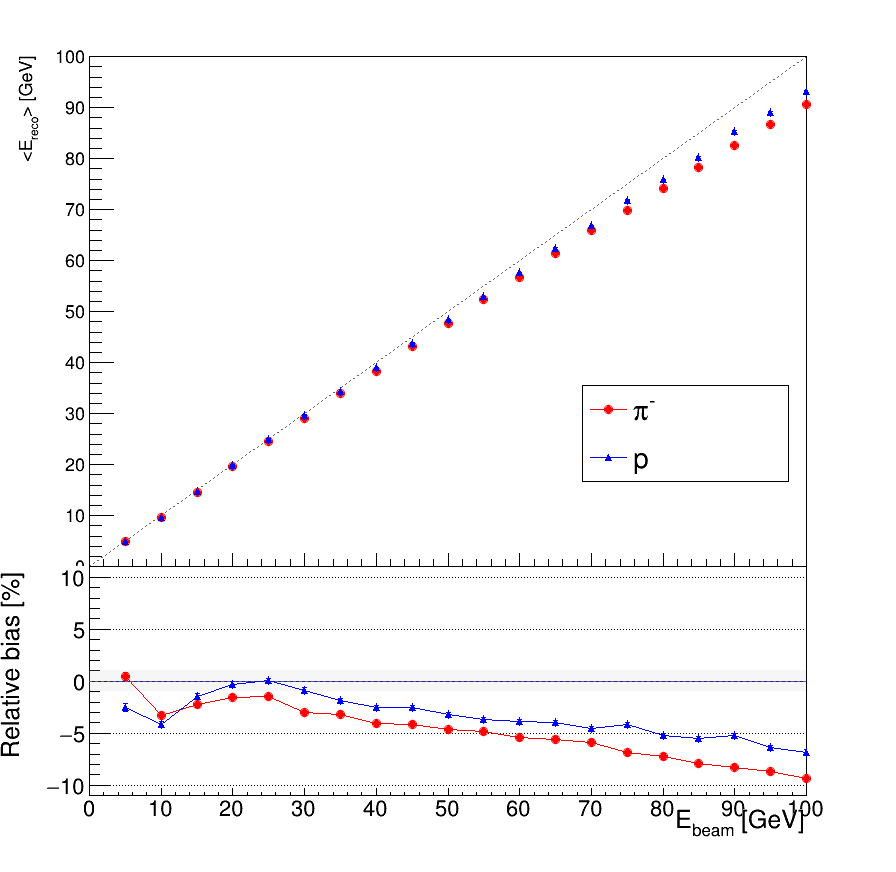
\includegraphics[width=0.78\linewidth]{Fig/no_PID_Lin_n_Dev_chi2.png}
\caption{Linéarité de la méthode paramétrique par minimisation du $\chi^2$. Haut : $\langle E_{\mathrm{reco}}\rangle$ en fonction de $E_{\mathrm{beam}}$. Bas : biais relatif.}
\label{fig:chi2-linearity}
\end{figure}

\subsection*{Résolution en énergie}

La Figure~\ref{fig:chi2-resolution} présente la résolution relative obtenue après ajustement gaussien des distributions de résidus.

Comme attendu pour un calorimètre hadronique, la résolution décroît rapidement avec l’énergie :

\begin{itemize}
    \item elle vaut environ $17$--$19\,\%$ vers 10 GeV ;
    \item elle passe sous $12\,\%$ vers 30 GeV ;
    \item elle atteint environ $8\,\%$ pour les pions et $7\,\%$ pour les protons à 100 GeV.
\end{itemize}

Cette évolution est compatible avec une loi dominée par un terme stochastique de type :

\[
\frac{\sigma(E)}{E}\approx\frac{a}{\sqrt{E}}\oplus b.
\]

Les protons présentent systématiquement une résolution légèrement meilleure que les pions, avec un gain typique de l’ordre de $0.5$ à $1$ point de pourcentage selon l’énergie. Cela suggère des fluctuations de gerbe un peu plus faibles ou une réponse plus stable dans le cadre de cette reconstruction.

\begin{figure}[!ht]
\centering
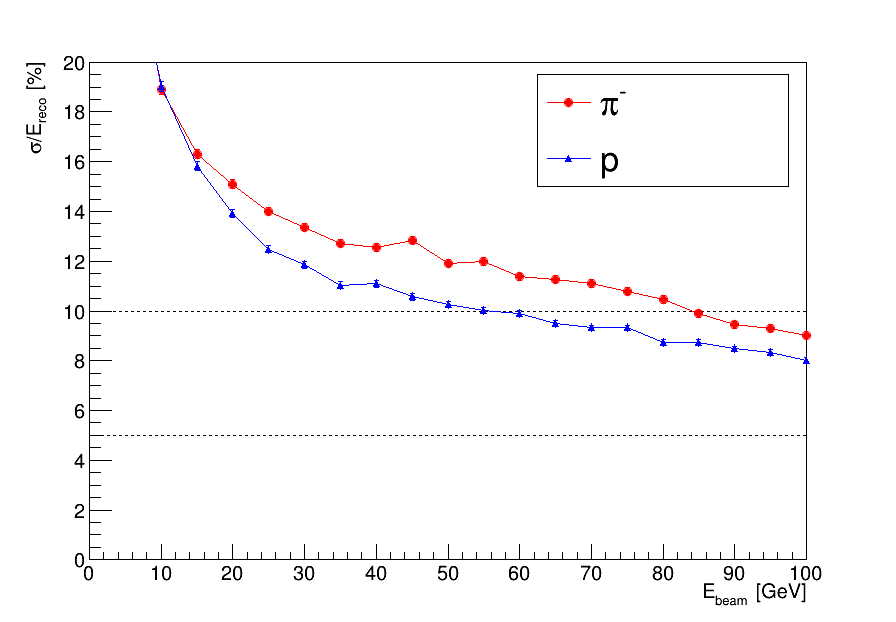
\includegraphics[width=0.78\linewidth]{Fig/no_PID_Resolution_relative_chi2.png}
\caption{Résolution relative obtenue avec la méthode paramétrique après fit gaussien des résidus.}
\label{fig:chi2-resolution}
\end{figure}

\subsection*{Discussion physique}

Ces résultats montrent que le simple comptage multi-seuils contient déjà une information calorimétrique riche. Malgré l’absence d’utilisation explicite de la topologie fine des hits, la combinaison pondérée de $N_1$, $N_2$ et $N_3$ permet :

\begin{itemize}
    \item une réponse globalement linéaire sur l’ensemble du domaine utile ;
    \item une résolution compétitive pour un calorimètre hadronique semi-digital ;
    \item une distinction visible entre espèces, en particulier au profit des protons.
\end{itemize}

Les écarts résiduels observés aux extrémités du domaine énergétique indiquent toutefois les limites intrinsèques d’une paramétrisation analytique simple. Les non-linéarités fines du détecteur et certaines corrélations complexes entre observables ne peuvent être décrites parfaitement par cette approche.

\subsection*{Bilan}

La méthode paramétrique calibrée par minimisation du $\chi^2$ constitue ainsi une base de reconstruction robuste, rapide et physiquement interprétable. Elle fournit déjà de bonnes performances entre 20 et 100 GeV, avec un biais limité et une résolution descendant jusqu’à $\sim7$--$8\,\%$ à haute énergie.

Elle sert naturellement de référence pour évaluer l’apport d’approches plus flexibles, en particulier la régression par arbres de décision boostés présentée dans la section suivante.

%%%%%%%%%%%%%%%%%

\section{Performances de la régression LightGBM}

Les performances de la régression par arbres de décision boostés sont évaluées sur le même échantillon indépendant que celui utilisé précédemment pour la méthode paramétrique, soit \(10\,000\) événements par point d’énergie entre 5 et 100~GeV. Cette procédure garantit une comparaison directe et équitable entre les deux approches.

Comme pour la calibration paramétrique, la régression supervisée est entraînée séparément pour chaque espèce étudiée. Deux modèles LightGBM indépendants sont ainsi construits : l’un dédié aux pions négatifs \(\pi^-\), l’autre aux protons \(p\), afin de tenir compte des différences de développement des gerbes hadroniques et d’optimiser la reconstruction dans chaque cas.

Les performances sont analysées selon deux critères principaux :

\begin{itemize}
    \item la \textbf{linéarité} de la réponse moyenne ;
    \item la \textbf{résolution relative}, extraite d’un ajustement gaussien des distributions de résidus.
\end{itemize}

\subsection*{Linéarité de la réponse}

La Figure~\ref{fig:bdt-linearity} présente la moyenne de l’énergie prédite en fonction de l’énergie incidente, ainsi que le biais relatif :

\[
\delta(E)=
\frac{\langle E_{\mathrm{pred}}\rangle-E_{\mathrm{beam}}}
{E_{\mathrm{beam}}}.
\]

La réponse suit globalement la diagonale idéale sur l’ensemble du domaine étudié. Entre 15 et 90~GeV, les écarts restent généralement limités à quelques pourcents, ce qui traduit une calibration satisfaisante sur la majeure partie de la gamme énergétique.

Trois régimes principaux peuvent être distingués :

\begin{itemize}
    \item \textbf{Très basses énergies :} un biais positif subsiste, lié aux fortes fluctuations statistiques lorsque la multiplicité de hits reste faible ;

    \item \textbf{Régime central :} la réponse devient très proche de la linéarité idéale, avec un biais voisin de zéro sur une large plage d’énergie ;

    \item \textbf{Hautes énergies :} une légère sous-réponse réapparaît, mais demeure modérée dans le domaine considéré.
\end{itemize}

Les protons conservent une réponse légèrement meilleure que les pions, bien que l’écart entre espèces reste limité.

\begin{figure}[!ht]
\centering
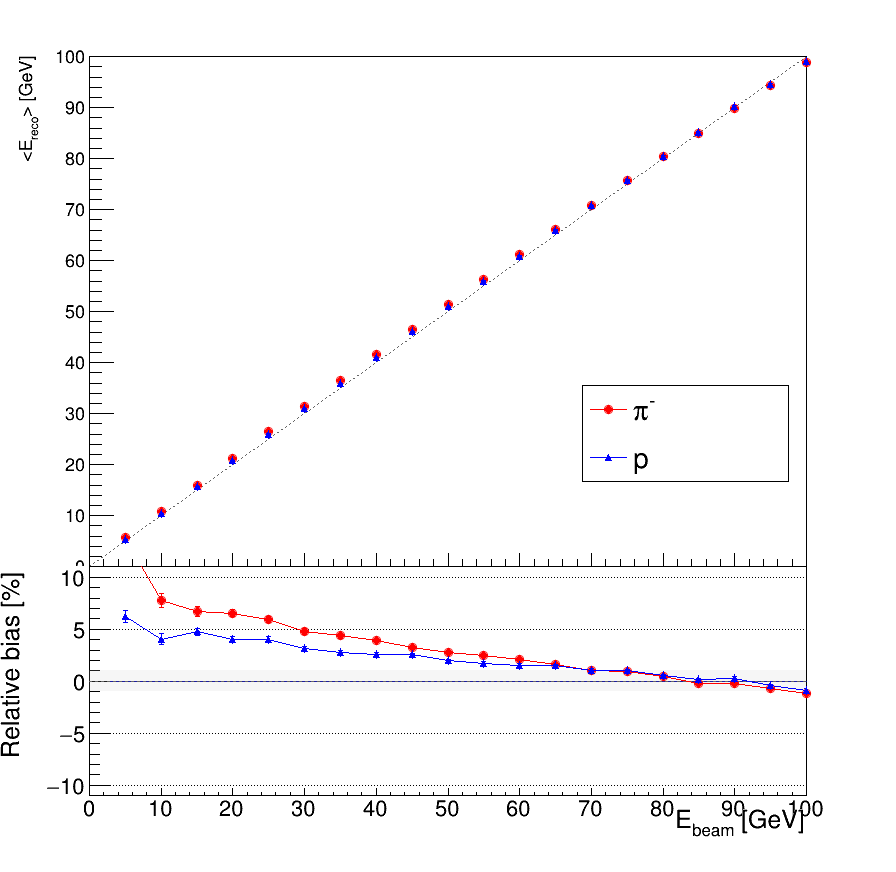
\includegraphics[width=0.78\linewidth]{Fig/no_PID_Lin_n_Dev_BDT.png}
\caption{Linéarité de la régression LightGBM. Haut : \(\langle E_{\mathrm{pred}}\rangle\) en fonction de \(E_{\mathrm{beam}}\). Bas : biais relatif.}
\label{fig:bdt-linearity}
\end{figure}

\subsection*{Résolution en énergie}

La Figure~\ref{fig:bdt-resolution} présente la résolution relative obtenue avec la régression LightGBM.

La tendance générale montre une amélioration progressive avec l’énergie :

\begin{itemize}
    \item environ \(19\,\%\) à 10~GeV ;
    \item proche de \(13\,\%\) vers 30~GeV ;
    \item de l’ordre de \(8\) à \(9\,\%\) à 100~GeV.
\end{itemize}

Les protons restent systématiquement mieux reconstruits que les pions, avec un avantage typique de quelques dixièmes à un point de pourcentage selon l’énergie.

Cette hiérarchie, déjà observée avec la méthode paramétrique, suggère que les fluctuations physiques propres aux gerbes hadroniques jouent un rôle réel, indépendamment de la méthode de reconstruction employée.

\begin{figure}[!ht]
\centering
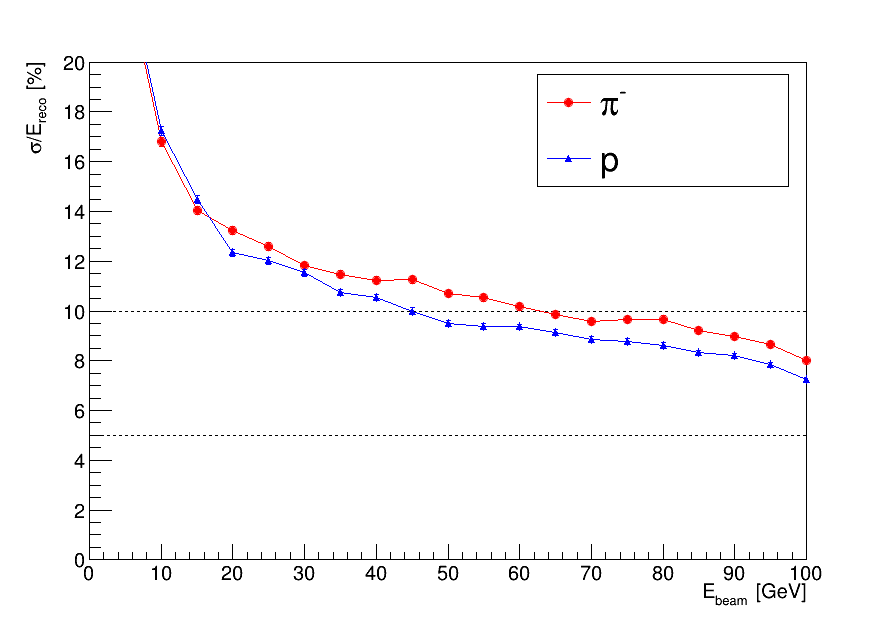
\includegraphics[width=0.78\linewidth]{Fig/no_PID_Resolution_relative_BDT.png}
\caption{Résolution relative obtenue avec la régression LightGBM après ajustement gaussien des résidus.}
\label{fig:bdt-resolution}
\end{figure}

\subsection*{Apport du modèle supervisé}

Par rapport à la méthode paramétrique, LightGBM apporte plusieurs bénéfices :

\begin{itemize}
    \item une plus grande flexibilité pour modéliser les non-linéarités de la réponse ;
    \item l’exploitation simultanée d’un grand nombre d’observables complémentaires ;
    \item une calibration stable sur la zone centrale en énergie ;
    \item des performances globalement comparables ou légèrement améliorées selon les bins considérés.
\end{itemize}

Le modèle apprend implicitement à combiner les informations longitudinales, spatiales et liées aux seuils afin de corriger certaines limites d’un simple comptage analytique.

\subsection*{Discussion physique}

Ces résultats confirment que la reconstruction de l’énergie ne dépend pas uniquement du nombre total de hits, mais également de la morphologie détaillée de la gerbe :

\begin{itemize}
    \item profondeur de première interaction ;
    \item densité locale ;
    \item étalement longitudinal ;
    \item compacité transverse ;
    \item répartition entre seuils.
\end{itemize}

Ces signatures supplémentaires sont naturellement exploitées par un modèle de boosting, ce qui explique ses bonnes performances et sa robustesse sur une large gamme d’énergie.

\subsection*{Bilan}

La régression LightGBM fournit ainsi une reconstruction performante, stable et compétitive sur l’ensemble du domaine étudié. Sans bouleverser l’ordre de grandeur des performances déjà obtenues par la méthode paramétrique, elle apporte une meilleure capacité d’adaptation aux structures complexes de la réponse calorimétrique.

Ces résultats motivent une comparaison directe avec la méthode analytique afin d’identifier plus précisément les domaines où chaque approche présente les meilleurs avantages.

\section{Comparaison entre méthode paramétrique et régression LightGBM}

Les deux approches étudiées dans ce chapitre poursuivent le même objectif : reconstruire l’énergie incidente à partir de la réponse du SDHCAL. Elles reposent toutefois sur des philosophies sensiblement différentes.

La méthode paramétrique s’appuie sur une formule analytique explicite fondée sur les compteurs multi-seuils \((N_1,N_2,N_3)\), dont les coefficients sont ajustés par minimisation du \(\chi^2\). À l’inverse, la régression LightGBM apprend directement, à partir des données simulées, la relation entre les observables de gerbe et l’énergie vraie.

Il est donc naturel de comparer leurs performances selon plusieurs critères complémentaires : linéarité, résolution, robustesse expérimentale et interprétabilité.

\subsection*{Linéarité de la réponse}

Les deux méthodes présentent une bonne linéarité globale sur l’intervalle 20--100~GeV, avec une réponse moyenne proche de la diagonale idéale.

La méthode paramétrique met en évidence :

\begin{itemize}
    \item une légère surestimation aux basses énergies ;
    \item une excellente stabilité dans la région intermédiaire ;
    \item une faible sous-réponse aux plus hautes énergies.
\end{itemize}

La régression LightGBM présente un comportement globalement comparable, avec par endroits une meilleure compensation locale des non-linéarités grâce à sa plus grande flexibilité.

En pratique, les deux approches offrent donc une calibration satisfaisante sur la majeure partie du domaine utile.

\subsection*{Résolution en énergie}

La différence la plus significative concerne la résolution relative.

La méthode paramétrique atteint déjà de bonnes performances, avec des valeurs typiques de :

\begin{itemize}
    \item \(17\) à \(19\,\%\) à basse énergie ;
    \item \(\sim 12\,\%\) vers 30~GeV ;
    \item \(\sim 7\) à \(8\,\%\) à 100~GeV.
\end{itemize}

La régression LightGBM fournit des performances du même ordre, avec selon les régions :

\begin{itemize}
    \item une amélioration modérée dans certains bins d’énergie ;
    \item une meilleure stabilité globale ;
    \item une exploitation plus complète des observables disponibles.
\end{itemize}

Le gain n’est donc pas spectaculaire, mais il reste réel et cohérent avec la richesse plus importante du modèle.

\subsection*{Dépendance à l’espèce hadronique}

Dans les deux approches, les protons sont légèrement mieux reconstruits que les pions sur l’ensemble du domaine énergétique.

Cette hiérarchie commune suggère qu’elle provient principalement des propriétés physiques des gerbes hadroniques, et non du choix de l’algorithme de reconstruction. Les fluctuations propres aux gerbes de pions semblent ainsi légèrement plus défavorables à la mesure calorimétrique.

\subsection*{Interprétabilité et simplicité}

La méthode paramétrique conserve plusieurs avantages pratiques :

\begin{itemize}
    \item formule explicite ;
    \item calibration rapide ;
    \item compréhension physique immédiate ;
    \item implémentation légère.
\end{itemize}

Elle constitue ainsi une solution robuste et facilement transférable.

À l’inverse, LightGBM offre :

\begin{itemize}
    \item une plus grande adaptabilité ;
    \item la prise en compte simultanée de nombreuses variables ;
    \item une calibration automatique plus puissante ;
    \item un potentiel de performance supérieur.
\end{itemize}

Son fonctionnement reste toutefois moins transparent qu’une paramétrisation analytique simple.

\subsection*{Robustesse expérimentale}

Dans une perspective expérimentale réelle, la méthode paramétrique peut se révéler plus simple à contrôler, car elle dépend d’un nombre limité de paramètres clairement identifiables.

La régression supervisée dépend davantage :

\begin{itemize}
    \item de la qualité des données simulées ;
    \item du domaine couvert par l’entraînement ;
    \item de la stabilité des variables d’entrée ;
    \item des dérives instrumentales éventuelles.
\end{itemize}

Une validation rigoureuse sur données réelles serait donc indispensable avant toute utilisation opérationnelle.

\subsection*{Synthèse comparative}

En résumé :

\begin{center}
\begin{tabular}{lcc}
\hline
Critère & Méthode \(\chi^2\) & LightGBM \\
\hline
Simplicité & Excellent & Bon \\
Interprétabilité & Excellent & Moyen \\
Linéarité & Très bonne & Très bonne \\
Résolution & Bonne & Très bonne \\
Flexibilité & Limitée & Excellente \\
Temps de développement & Faible & Plus élevé \\
\hline
\end{tabular}
\end{center}

\subsection*{Bilan}

La méthode paramétrique constitue une base robuste, rapide et physiquement lisible. La régression LightGBM permet d’aller plus loin en exploitant davantage l’information contenue dans les gerbes et en corrigeant plus finement certaines non-linéarités.

Le choix entre les deux dépend donc du contexte visé :

\begin{itemize}
    \item calibration simple et maîtrisable : avantage à la méthode paramétrique ;
    \item performance maximale : avantage à LightGBM ;
    \item stratégie hybride : combinaison des deux approches.
\end{itemize}

Ces résultats ouvrent naturellement la voie à une chaîne de reconstruction plus complète combinant identification des particules et estimation de l’énergie.

%%%%%%%%%%%%%%%%%%%%
\section{Discussion physique, limites et perspectives}

Les résultats obtenus dans ce chapitre montrent que le SDHCAL possède un potentiel réel pour la reconstruction de l’énergie hadronique, aussi bien à travers une calibration analytique simple qu’au moyen de méthodes modernes d’apprentissage supervisé. Les performances atteintes sont globalement satisfaisantes sur la gamme 5--100~GeV, avec une bonne linéarité moyenne et une résolution relative descendant sous les \(10\,\%\) aux plus hautes énergies.

Ces résultats doivent toutefois être replacés dans leur contexte physique et méthodologique.

\subsection*{Origine physique des limitations}

La reconstruction de l’énergie hadronique demeure intrinsèquement plus difficile que celle des gerbes électromagnétiques. Plusieurs mécanismes fondamentaux limitent la précision accessible :

\begin{itemize}
    \item fortes fluctuations de la première interaction nucléaire ;
    \item production variable de composantes neutres partiellement invisibles ;
    \item fraction électromagnétique fluctuante d’un événement à l’autre ;
    \item pertes d’énergie hors acceptance latérale ;
    \item fuites longitudinales aux plus hautes énergies.
\end{itemize}

Même avec un détecteur granulaire performant, ces fluctuations imposent une limite physique à la résolution mesurable.

\subsection*{Spécificités du SDHCAL}

Le SDHCAL présente néanmoins plusieurs atouts majeurs :

\begin{itemize}
    \item granularité fine permettant de suivre la topologie détaillée des gerbes ;
    \item lecture multi-seuils apportant une estimation locale de densité ;
    \item grand nombre de canaux améliorant la robustesse statistique ;
    \item potentiel d’exploitation conjointe des informations spatiales et temporelles.
\end{itemize}

En contrepartie, la lecture semi-digitale ne fournit pas une mesure continue de l’énergie déposée cellule par cellule. Une partie de l’information calorimétrique brute est donc perdue par rapport à un calorimètre entièrement analogique.

\subsection*{Limites de la méthode paramétrique}

La calibration par minimisation du \(\chi^2\) reste particulièrement attractive par sa simplicité, mais elle présente plusieurs limites :

\begin{itemize}
    \item dépendance à la forme fonctionnelle choisie ;
    \item difficulté à absorber des non-linéarités fines ;
    \item utilisation restreinte à un petit nombre d’observables ;
    \item sensibilité possible aux corrélations entre paramètres ajustés.
\end{itemize}

Elle constitue ainsi une excellente référence physique, sans nécessairement représenter l’optimum absolu en performance.

\subsection*{Limites de l’approche LightGBM}

La régression supervisée offre une flexibilité supérieure, mais introduit d’autres contraintes :

\begin{itemize}
    \item dépendance à la qualité et au réalisme des données simulées ;
    \item risque de perte de robustesse hors du domaine couvert par l’entraînement ;
    \item interprétation physique moins immédiate ;
    \item nécessité de contrôler la stabilité des variables d’entrée.
\end{itemize}

Une bonne performance sur simulation ne garantit donc pas automatiquement une performance identique sur données réelles.

\subsection*{Contrôles indispensables pour une application réelle}

Avant toute utilisation expérimentale, plusieurs validations seraient nécessaires :

\begin{itemize}
    \item comparaison détaillée simulation / données réelles ;
    \item étude de robustesse face au bruit électronique ;
    \item impact des inefficacités de détection ;
    \item variations de calibration entre couches ;
    \item dépendance au modèle hadronique utilisé en simulation.
\end{itemize}

Ces effets peuvent influencer directement la réponse reconstruite et doivent être maîtrisés.

\subsection*{Perspectives d’amélioration}

Plusieurs pistes naturelles se dégagent pour prolonger ce travail :

\begin{itemize}
    \item calibration dépendante de l’énergie ou de la topologie de la gerbe ;
    \item combinaison de la méthode \(\chi^2\) et du modèle LightGBM ;
    \item modèles spécialisés selon l’espèce hadronique ;
    \item exploitation plus poussée de l’information temporelle ;
    \item réseaux neuronaux 3D ou graphes de hits.
\end{itemize}

Une stratégie hybride paraît particulièrement prometteuse : utiliser la robustesse physique de la méthode paramétrique comme entrée supplémentaire d’un modèle supervisé plus flexible.

\subsection*{Lien avec le Particle Flow}

Dans une chaîne de reconstruction moderne, la mesure calorimétrique ne constitue qu’un élément d’un système global. Elle s’intègre naturellement aux approches de type \emph{Particle Flow}, où :

\begin{itemize}
    \item les particules chargées sont principalement mesurées par le trajectographe ;
    \item les photons par le calorimètre électromagnétique ;
    \item les hadrons neutres dépendent fortement des performances du HCAL.
\end{itemize}

Une reconstruction hadronique performante dans le SDHCAL revêt donc une importance stratégique, en particulier pour la mesure précise de la composante neutre des jets.

\subsection*{Bilan}

L’étude présentée ici montre qu’un calorimètre semi-digital hautement granulaire peut atteindre de très bonnes performances malgré les contraintes propres aux interactions hadroniques.

Les approches paramétriques assurent robustesse, rapidité et lisibilité physique, tandis que les méthodes supervisées ouvrent la voie à des gains supplémentaires. L’enjeu futur ne réside donc pas uniquement dans la performance brute, mais dans la capacité à transférer ces méthodes vers des conditions expérimentales réalistes et vers la reconstruction globale d’événements complexes.

%%%%%%%%%%%%%%
\section{Conclusion}

Ce chapitre était consacré à la reconstruction de l’énergie hadronique dans le SDHCAL à partir de gerbes simulées de pions négatifs $\pi^-$ et de protons, sur une gamme d’énergie comprise entre 5 et 100~GeV. L’objectif principal était d’évaluer dans quelle mesure la granularité fine et la lecture semi-digitale du détecteur permettent d’obtenir une mesure calorimétrique précise malgré les fluctuations intrinsèques des interactions hadroniques.

Deux approches complémentaires ont été étudiées.

La première repose sur une \textbf{méthode paramétrique} fondée sur les nombres de hits associés aux trois seuils semi-digitaux. Les coefficients de pondération sont ajustés par minimisation du $\chi^2$. Cette stratégie, simple et physiquement interprétable, fournit une réponse globalement linéaire sur la majeure partie du domaine étudié, avec une résolution relative atteignant environ $7$ à $8\,\%$ aux plus hautes énergies.

La seconde repose sur une \textbf{régression supervisée par arbres de décision boostés}, implémentée via LightGBM. En exploitant un ensemble plus riche d’observables décrivant la morphologie des gerbes, cette méthode apporte une plus grande flexibilité de calibration et permet des performances globalement comparables, voire légèrement supérieures selon les régions en énergie considérées.

La comparaison entre les deux approches met en évidence un résultat important : une part significative de l’information énergétique est déjà contenue dans les simples compteurs multi-seuils du SDHCAL. Toutefois, l’ajout de variables liées au développement longitudinal, à la densité locale ou à la compacité permet de mieux corriger certaines non-linéarités résiduelles et d’exploiter plus finement la structure des gerbes.

Les protons apparaissent légèrement mieux reconstruits que les pions sur l’ensemble du domaine étudié, ce qui suggère des fluctuations de gerbe plus favorables dans le cadre de cette mesure. Cette hiérarchie, observée de manière cohérente avec les deux méthodes, semble donc principalement liée aux propriétés physiques des interactions hadroniques plutôt qu’au choix de l’algorithme de reconstruction.

Au-delà des performances numériques, cette étude confirme que le concept de calorimètre hadronique semi-digital hautement granulaire constitue une solution crédible pour la calorimétrie de précision des futurs détecteurs. Il combine richesse topologique, robustesse instrumentale et fort potentiel pour les approches modernes d’apprentissage automatique.

Enfin, les résultats obtenus ici prolongent naturellement ceux du chapitre précédent consacré à l’identification des particules. Ils ouvrent la voie à une chaîne de reconstruction plus complète combinant \textbf{identification hadronique et estimation d’énergie} sur des échantillons mixtes, étape essentielle dans la perspective d’une reconstruction globale d’événements complexes et des futures analyses de type \emph{Particle Flow}.

\chapter{Analyse sur échantillons mixtes}
\label{sec:analyse_mixte}

\section{Motivation et cadre réaliste}
\label{sec:motivation_mixte}

Les chapitres précédents ont permis d’étudier séparément deux problématiques complémentaires : l’identification des particules hadroniques dans le SDHCAL, puis la reconstruction de leur énergie incidente. Dans ces études préliminaires, chaque espèce de particule était traitée indépendamment, ce qui revient à supposer connue a priori la nature de la particule entrant dans le calorimètre.

Une telle hypothèse constitue un cadre idéalisé, utile pour caractériser les performances intrinsèques des méthodes développées, mais elle reste insuffisante dans la perspective d’une utilisation expérimentale réaliste. En pratique, un détecteur reçoit simultanément différentes espèces de particules, et l’information disponible en amont ne permet pas toujours de distinguer immédiatement un pion, un proton ou un hadron neutre. La reconstruction de l’énergie doit alors être effectuée dans un contexte où l’identité de la particule n’est pas connue avec certitude.

Cette situation introduit un couplage direct entre les deux tâches étudiées précédemment :

\begin{itemize}
    \item \textbf{identifier} la particule incidente à partir de la topologie de sa gerbe ;
    \item \textbf{reconstruire} son énergie en appliquant la calibration la plus adaptée.
\end{itemize}

Autrement dit, la qualité de la reconstruction énergétique dépend désormais de la qualité du classificateur PID. Une erreur d’identification peut conduire à appliquer un estimateur optimisé pour une autre espèce, et donc introduire un biais systématique sur l’énergie reconstruite.

Cet enjeu est particulièrement important dans les approches modernes de type \emph{Particle Flow Algorithm} (PFA), où la reconstruction globale d’un événement repose sur la combinaison cohérente de plusieurs sous-détecteurs. Dans ce cadre, une bonne identification hadronique améliore non seulement la pureté des objets reconstruits, mais aussi la précision de la mesure énergétique associée.

L’objectif de ce chapitre est donc d’évaluer les performances d’une chaîne complète de reconstruction dans un environnement mixte, plus proche des conditions expérimentales réelles. Trois stratégies sont comparées :

\begin{itemize}
    \item une chaîne \textbf{PID + régression LightGBM}, où l’espèce prédite détermine le modèle d’énergie utilisé ;
    
    \item une chaîne \textbf{PID + méthode paramétrique}, fondée sur les calibrations analytiques spécifiques à chaque espèce ;
    
    \item une approche de référence consistant à appliquer une \textbf{calibration unique issue des pions} à toutes les particules, sans identification préalable.
\end{itemize}

La comparaison de ces scénarios permet de quantifier l’apport réel du PID sur la reconstruction calorimétrique, d’identifier les limitations dues aux confusions entre espèces, et d’évaluer quelles stratégies apparaissent les plus robustes pour une application future sur données réalistes.

%%%%%%%%%%%%%%%%%%%%%%%%%%%%%%%%%%%%%%%%%%%%%%%%%%%
\section{Chaîne complète : PID + régression BDT}
\label{subsec:mix_pid_bdt}

La première stratégie étudiée consiste à combiner le classificateur de particules présenté au chapitre précédent avec les modèles de régression LightGBM dédiés à la reconstruction d’énergie. Pour chaque événement du faisceau mixte, une étape d’identification est d’abord réalisée entre les classes pion \(\pi^-\) et proton \(p\). L’énergie est ensuite estimée à l’aide du modèle de régression correspondant à l’espèce prédite.

Cette approche reproduit un scénario réaliste dans lequel plusieurs calibrations spécialisées sont disponibles, mais où leur sélection dépend directement de la performance du PID.

\subsection*{Linéarité de la réponse}

La Figure~\ref{fig:linearite_pid_bdt_new} présente la moyenne de l’énergie reconstruite en fonction de l’énergie vraie, ainsi que le biais relatif défini par :

\[
\delta(E)=
\frac{\langle E_{\mathrm{reco}}\rangle-E_{\mathrm{true}}}{E_{\mathrm{true}}}.
\]

Globalement, la réponse reconstruite reste très proche de la diagonale idéale sur l’ensemble du domaine étudié. Les deux espèces suivent une évolution régulière, sans rupture visible, ce qui confirme la stabilité de la chaîne complète PID + régression.

À basse énergie, un léger biais positif est observé. Il atteint environ \(+10\,\%\) pour les pions autour de \SI{10}{GeV}, tandis qu’il reste plus modéré pour les protons (\(\sim +3\) à \(+4\,\%\)). Cette surestimation diminue progressivement avec l’énergie.

Entre \SIrange{40}{80}{GeV}, le biais devient faible pour les deux classes, généralement contenu dans une bande de quelques pourcents autour de zéro. Cette région correspond au domaine où les performances globales du modèle sont les meilleures.

À plus haute énergie, une légère sous-réponse apparaît. À \SI{100}{GeV}, elle reste toutefois modérée, de l’ordre de \(-1\) à \(-2\,\%\), ce qui traduit une excellente linéarité globale.

\begin{figure}[!ht]
\centering
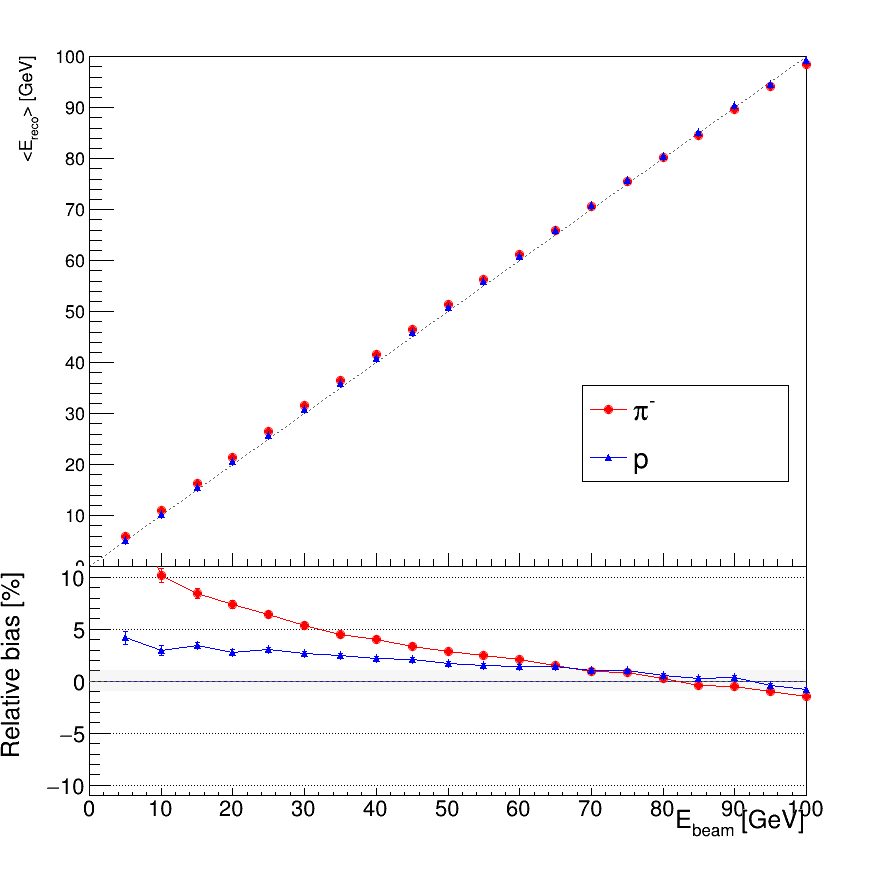
\includegraphics[width=0.78\linewidth]{Fig/PID_Lin_n_Dev_BDT.png}
\caption{Linéarité de la reconstruction d’énergie et biais relatif pour la chaîne complète \textbf{PID + BDT}. Les pions sont représentés en rouge et les protons en bleu.}
\label{fig:linearite_pid_bdt_new}
\end{figure}

\subsection*{Résolution énergétique}

La Figure~\ref{fig:resolution_pid_bdt_new} montre l’évolution de la résolution relative :

\[
\frac{\sigma_E}{E},
\]

extraite à partir d’un ajustement gaussien des distributions résiduelles dans chaque bin d’énergie.

Comme attendu pour un calorimètre hadronique, la résolution décroît rapidement lorsque l’énergie augmente. Elle passe d’environ \(19\,\%\) à basse énergie à des valeurs proches de \(8\,\%\) autour de \SI{100}{GeV}.

Les protons présentent systématiquement une résolution légèrement meilleure que celle des pions, avec un avantage typique de quelques dixièmes à un point de pourcentage selon l’énergie. Cette hiérarchie est cohérente avec les observations faites dans le cas idéal, où les gerbes protoniques apparaissaient légèrement plus stables.

À haute énergie, les deux courbes convergent vers des performances très proches, signe que l’impact des erreurs de PID devient secondaire lorsque la statistique de gerbe augmente.

\begin{figure}[!ht]
\centering
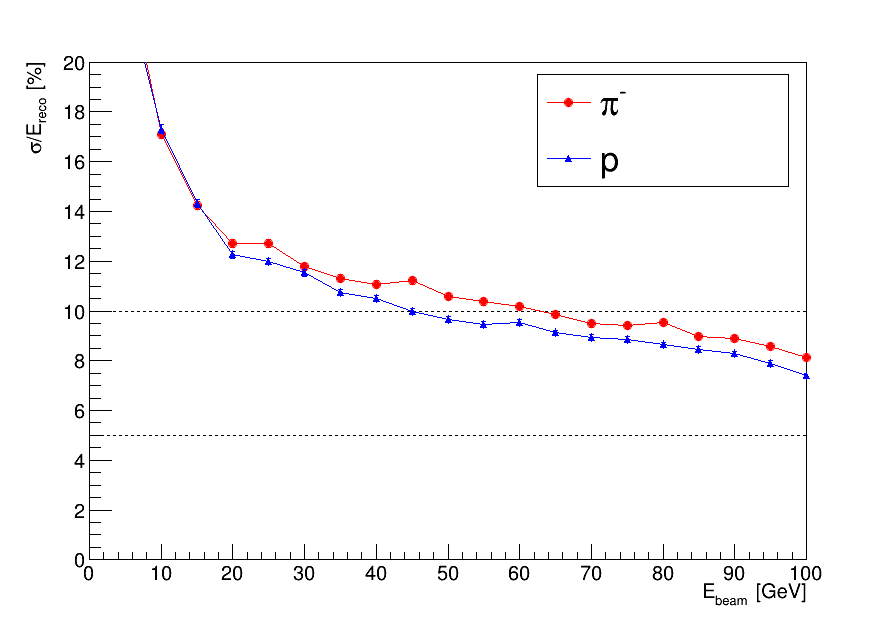
\includegraphics[width=0.78\linewidth]{Fig/PID_Resolution_relative_BDT.png}
\caption{Résolution relative \(\sigma(E)/E\) obtenue avec la chaîne \textbf{PID + BDT}.}
\label{fig:resolution_pid_bdt_new}
\end{figure}

\subsection*{Interprétation physique}

Ces résultats montrent que la combinaison d’un PID supervisé avec une régression dédiée par espèce permet de conserver l’essentiel des performances obtenues dans le scénario idéal où la particule est supposée connue.

Le biais positif observé à basse énergie peut s’expliquer par la faible multiplicité de hits et par les fluctuations importantes des premières interactions hadroniques, qui rendent simultanément l’identification et la régression plus délicates.

La légère supériorité des protons en résolution suggère que leurs gerbes sont, dans cette configuration, un peu mieux modélisées par les variables d’entrée utilisées pour la régression.

Enfin, la faiblesse des biais résiduels à moyenne et haute énergie indique que les erreurs de classification pion/proton n’induisent qu’une dégradation limitée sur la reconstruction finale.

\subsection*{Bilan}

Parmi les stratégies étudiées, la chaîne \textbf{PID + BDT} apparaît comme la plus performante et la plus robuste. Elle combine une excellente linéarité, une résolution compétitive sur tout le domaine énergétique, et une faible sensibilité aux confusions résiduelles du classificateur. Elle constitue ainsi une référence solide pour une reconstruction hadronique réaliste dans le SDHCAL.
%%%%%%%%%%%%%%%%%%%%%%%%%%%%%%%%%%%%%%%%%%%%%%%%%%%%%

\section{Chaîne complète : PID + reconstruction paramétrique}
\label{subsec:mix_pid_param}

La seconde stratégie consiste à conserver la même étape d’identification des particules, mais à remplacer la régression par arbres boostés par la méthode analytique fondée sur les compteurs semi-digitaux aux trois seuils. Une fois la particule classée comme pion \(\pi^-\) ou proton \(p\), les coefficients de calibration spécifiques à cette espèce sont appliqués afin d’estimer l’énergie incidente.

Cette approche est plus simple et plus interprétable que la régression BDT. Elle permet également d’évaluer dans quelle mesure une calibration paramétrique classique reste compétitive lorsqu’elle est couplée à une étape de PID.

\subsection*{Linéarité de la réponse}

La Figure~\ref{fig:linearite_pid_param_new} présente la réponse moyenne reconstruite ainsi que le biais relatif en fonction de l’énergie vraie.

La tendance générale reste linéaire sur l’ensemble du domaine étudié, mais un biais négatif apparaît progressivement lorsque l’énergie augmente. Après une zone relativement bien calibrée entre \SIrange{20}{50}{GeV}, les deux espèces présentent une sous-réponse croissante.

À \SI{100}{GeV}, le biais atteint environ \(-9\,\%\) pour les pions et \(-7\,\%\) pour les protons. Cette déviation est nettement plus marquée que dans le cas de la chaîne PID + BDT.

À basse énergie, la situation reste satisfaisante : les points les plus bas en énergie sont proches de la diagonale idéale, avec seulement de faibles écarts.

\begin{figure}[!ht]
\centering
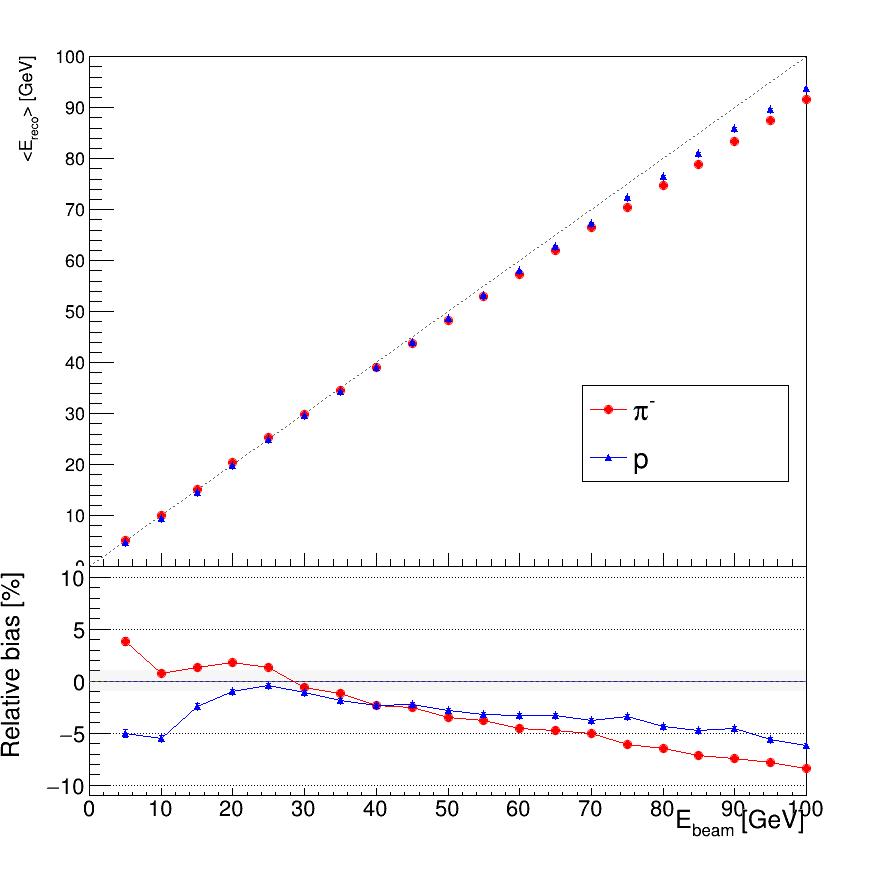
\includegraphics[width=0.78\linewidth]{Fig/PID_Lin_n_Dev_chi2.png}
\caption{Linéarité de la reconstruction et biais relatif pour la chaîne \textbf{PID + méthode paramétrique}.}
\label{fig:linearite_pid_param_new}
\end{figure}

\subsection*{Résolution énergétique}

La Figure~\ref{fig:resolution_pid_param_new} montre la résolution relative \(\sigma(E)/E\).

Le comportement suit la décroissance attendue avec l’énergie, passant d’environ \(19\,\%\) à basse énergie à des valeurs proches de \(9\,\%\) autour de \SI{100}{GeV}. Les performances restent donc globalement bonnes.

Les protons conservent une légère avance sur les pions sur la quasi-totalité du domaine énergétique, avec un écart modéré mais systématique. La hiérarchie observée est similaire à celle du cas BDT.

Cependant, à énergie élevée, la résolution reste légèrement moins bonne que celle obtenue avec la régression LightGBM.

\begin{figure}[!ht]
\centering
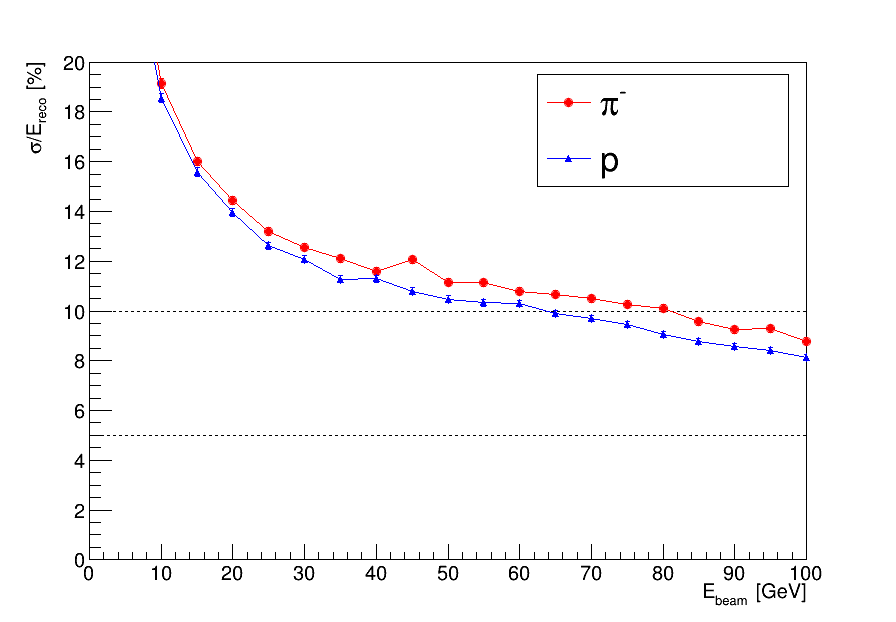
\includegraphics[width=0.78\linewidth]{Fig/PID_Resolution_relative_chi2.png}
\caption{Résolution relative \(\sigma(E)/E\) pour la chaîne \textbf{PID + méthode paramétrique}.}
\label{fig:resolution_pid_param_new}
\end{figure}

\subsection*{Interprétation physique}

Ces résultats montrent que la méthode paramétrique conserve une bonne robustesse statistique, même en présence d’une étape de PID en amont. Les performances restent proches de celles du scénario idéal, ce qui confirme la pertinence physique des observables basées sur les trois seuils semi-digitaux.

La sous-réponse croissante à haute énergie reflète néanmoins les limites intrinsèques de la paramétrisation analytique retenue. Lorsque les gerbes deviennent plus développées et plus fluctuantes, une combinaison polynomiale simple des compteurs \(N_1\), \(N_2\) et \(N_3\) ne suffit plus toujours à corriger les effets de saturation ou de non-linéarité.

La légère supériorité des protons suggère à nouveau une réponse plus régulière de leurs gerbes dans le calorimètre.

\subsection*{Bilan}

La chaîne \textbf{PID + méthode paramétrique} fournit une reconstruction d’énergie compétitive, simple à mettre en œuvre et physiquement interprétable. Elle reste toutefois limitée par un biais croissant aux hautes énergies et par une résolution légèrement inférieure à celle obtenue avec la stratégie PID + BDT. Elle constitue donc une solution robuste, mais moins performante que l’approche fondée sur l’apprentissage supervisé.
%%%%%%%%%%%%%%%%%%%%%%%%%%%%%%%%%%%%%%%%%%%%%%%%%%%%%
\section{Calibration pion appliquée à toutes les espèces}
\label{subsec:param_pion_to_all_new}

La troisième stratégie étudiée sert de référence simplifiée. Elle consiste à utiliser une unique calibration déterminée sur les pions \(\pi^-\), puis à l’appliquer indistinctement à tous les événements du faisceau mixte, y compris lorsqu’ils correspondent à des protons.

Une telle méthode ne nécessite aucune étape préalable d’identification des particules. Elle représente donc une solution opérationnellement simple, mais potentiellement sensible aux différences physiques entre espèces hadroniques.

L’objectif de cette étude est de quantifier le gain réel apporté par le PID en comparant cette calibration unique aux deux approches précédentes.

\subsection*{Linéarité de la réponse}

La Figure~\ref{fig:linearite_pion_all_new} montre la réponse moyenne reconstruite et le biais relatif obtenu avec cette calibration universelle.

Les pions, utilisés pour déterminer les coefficients, restent naturellement les mieux reconstruits. Leur biais reste modéré sur une large partie du domaine énergétique, avec une réponse proche de la diagonale idéale jusqu’aux énergies intermédiaires.

En revanche, les protons présentent un décalage systématique négatif beaucoup plus marqué. Après une région relativement correcte autour de \SIrange{20}{30}{GeV}, la sous-réponse augmente progressivement avec l’énergie pour atteindre environ \(-6\,\%\) à \SI{100}{GeV}.

Cette différence entre espèces met clairement en évidence qu’une calibration optimisée pour les pions ne peut être transposée sans perte aux protons.

\begin{figure}[!ht]
\centering
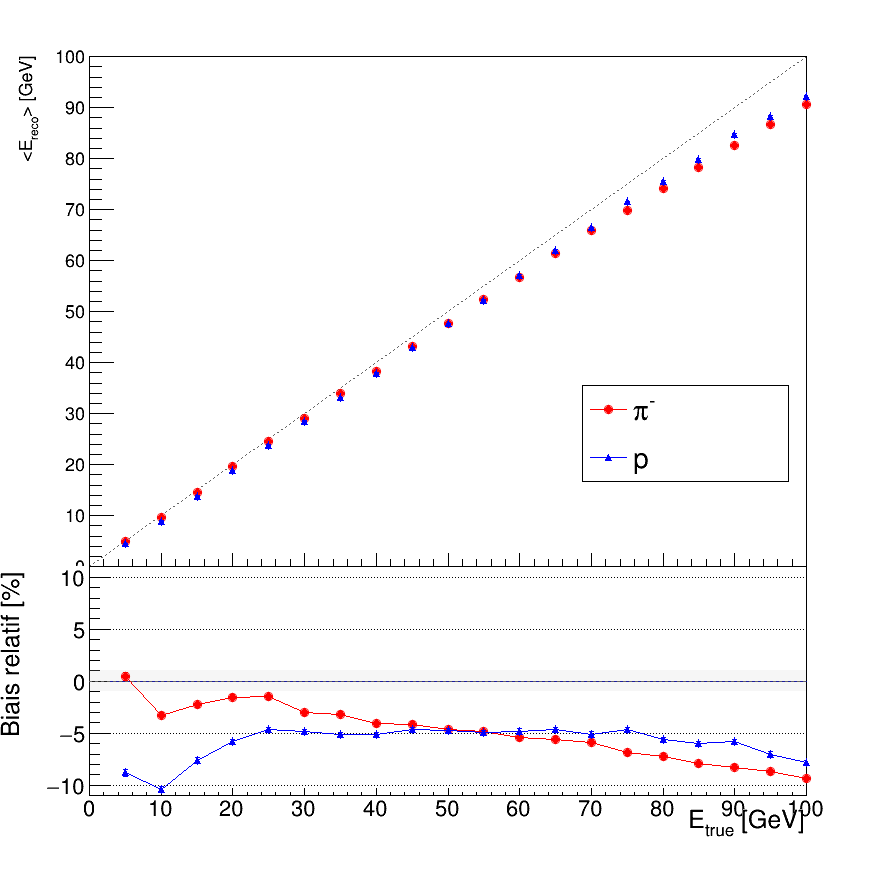
\includegraphics[width=0.78\linewidth]{Fig/PID_Lin_n_Dev_chi2_pion.png}
\caption{Linéarité de la reconstruction et biais relatif lorsqu’une calibration ajustée sur les pions est appliquée à toutes les espèces.}
\label{fig:linearite_pion_all_new}
\end{figure}

\subsection*{Résolution énergétique}

La Figure~\ref{fig:resolution_pion_all_new} présente la résolution relative \(\sigma(E)/E\).

Les performances restent globalement correctes et suivent la décroissance attendue avec l’énergie. À \SI{100}{GeV}, la résolution atteint des valeurs proches de \(8\) à \(9\,\%\), comparables aux autres approches.

Les protons gardent même une légère avance sur les pions en résolution pure, malgré leur biais systématique plus important. Cela montre qu’une bonne résolution ne garantit pas nécessairement une réponse correctement calibrée.

\begin{figure}[!ht]
\centering
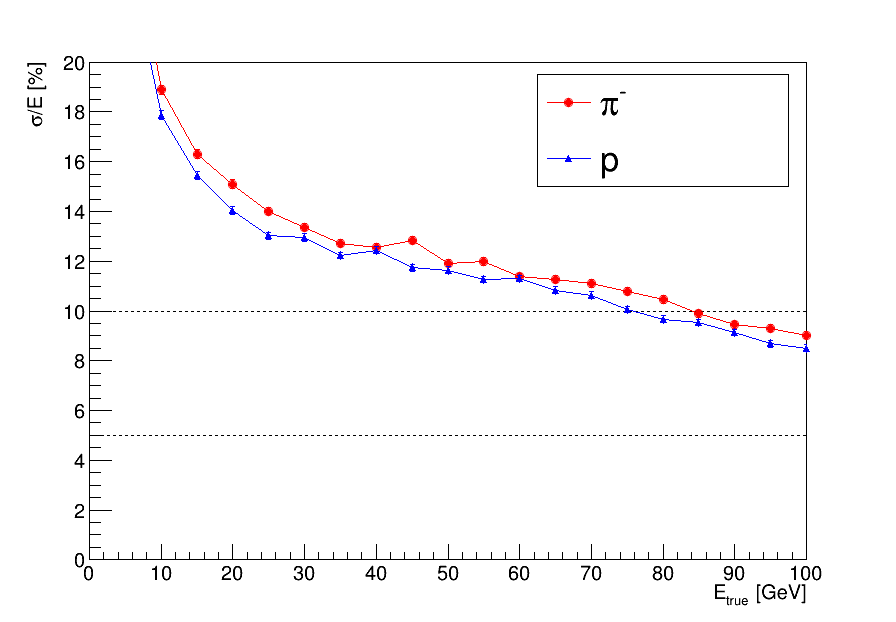
\includegraphics[width=0.78\linewidth]{Fig/PID_Resolution_relative_chi2_pion.png}
\caption{Résolution relative \(\sigma(E)/E\) obtenue avec une calibration pion appliquée à tous les événements.}
\label{fig:resolution_pion_all_new}
\end{figure}

\subsection*{Interprétation physique}

Ce comportement est cohérent avec les différences de développement des gerbes hadroniques selon l’espèce incidente. Les protons ne déposent pas leur énergie selon exactement les mêmes profils que les pions : profondeur moyenne d’interaction, fraction électromagnétique et densité locale peuvent différer.

Une calibration unique absorbe correctement la réponse moyenne des pions, mais ne capture pas ces spécificités pour les protons, d’où le biais observé.

Cette étude démontre ainsi que le PID n’améliore pas seulement l’étiquetage des événements : il permet aussi de sélectionner une calibration énergétique adaptée, ce qui réduit directement les biais systématiques.

\subsection*{Bilan}

L’approche par calibration unique constitue une base simple et raisonnablement performante en résolution, mais elle introduit un biais dépendant de l’espèce, particulièrement visible pour les protons aux hautes énergies.

Elle représente donc une solution de référence utile, mais inférieure aux stratégies exploitant explicitement l’identification des particules avant la reconstruction de l’énergie.
%%%%%%%%%%%%%%%%%%%%%%%%%%%%%%%%%%%%%%%%%%%%%%%%%%%%%%
\section{Comparaison globale des approches}
\label{subsec:comparaison_mixte}

Les trois stratégies étudiées permettent toutes de reconstruire l’énergie incidente avec des performances globalement satisfaisantes. Des différences nettes apparaissent toutefois lorsqu’on compare simultanément la linéarité de la réponse, la résolution énergétique et la robustesse vis-à-vis du mélange d’espèces.

L’intérêt de cette comparaison n’est donc pas uniquement de désigner la méthode la plus performante, mais d’identifier le meilleur compromis entre précision calorimétrique, simplicité de mise en œuvre et capacité d’adaptation à un environnement expérimental réaliste.

\subsection*{Linéarité et biais}

La chaîne \textbf{PID + LightGBM} fournit la réponse la plus proche du comportement idéal. Le biais reste faible sur la majeure partie du domaine énergétique, généralement contenu dans quelques pourcents, avec seulement une légère surestimation aux basses énergies et une faible sous-réponse à \SI{100}{GeV}.

La stratégie \textbf{PID + méthode paramétrique} conserve une bonne linéarité globale, mais présente une dérive négative progressive lorsque l’énergie augmente. Cette tendance traduit les limites d’une paramétrisation analytique fixe face à l’évolution de la morphologie des gerbes avec l’énergie.

Enfin, la \textbf{calibration pion appliquée à toutes les espèces} met en évidence un biais dépendant de la nature de la particule. Les pions restent correctement reconstruits, tandis que les protons subissent une sous-estimation systématique croissante avec l’énergie.

Ainsi, l’identification préalable des particules réduit clairement les biais de calibration inter-espèces et améliore la stabilité globale de la réponse.

\subsection*{Résolution énergétique}

Les trois approches présentent une décroissance régulière de la résolution relative avec l’énergie, conforme au comportement attendu d’un calorimètre hadronique.

La chaîne \textbf{PID + LightGBM} atteint les meilleures performances globales, avec une résolution proche de \(8\,\%\) aux plus hautes énergies.

La méthode \textbf{PID + paramétrique} reste légèrement en retrait, avec des valeurs proches de \(9\,\%\) autour de \SI{100}{GeV}.

La \textbf{calibration pion universelle} conserve une résolution du même ordre de grandeur, ce qui montre que la dispersion statistique reste correctement maîtrisée même lorsqu’un biais moyen subsiste.

Ces observations soulignent qu’une bonne résolution ne garantit pas, à elle seule, une reconstruction correctement calibrée : la maîtrise du biais constitue un critère tout aussi essentiel.

\subsection*{Apport spécifique du PID}

L’un des enseignements majeurs de cette étude est que le PID n’intervient pas uniquement comme outil de classification, mais également comme levier direct d’amélioration de la reconstruction calorimétrique.

En distinguant les pions des protons avant l’estimation de l’énergie, il devient possible d’appliquer une calibration cohérente avec la physique propre à chaque espèce. Le bénéfice se manifeste principalement par une réduction des biais systématiques, particulièrement visible dans la comparaison avec la calibration unique issue des pions.

Les erreurs résiduelles du classificateur limitent naturellement ce gain potentiel, mais leur impact reste modéré dans les performances observées ici.

\subsection*{Choix de la stratégie optimale}

Au regard des résultats obtenus :

\begin{itemize}
    \item la chaîne \textbf{PID + LightGBM} apparaît comme la solution la plus performante et la plus polyvalente dans le cadre de cette étude ;
    
    \item la chaîne \textbf{PID + paramétrique} constitue une alternative robuste, plus simple et plus directement interprétable ;
    
    \item la \textbf{calibration pion unique} peut servir de référence minimale ou de solution de secours, mais reste pénalisée par un biais dépendant de l’espèce incidente.
\end{itemize}

Le choix final dépend donc du contexte visé : recherche de performance maximale, besoin de simplicité opérationnelle, ou exigence de contrôle systématique renforcé.

\subsection*{Bilan}

Dans un environnement expérimental réaliste, la combinaison d’un PID supervisé et d’un estimateur d’énergie spécialisé apparaît comme la stratégie la plus pertinente. Elle permet d’exploiter simultanément la richesse topologique du SDHCAL pour identifier la particule incidente et améliorer la précision de la mesure énergétique.

Ces résultats confirment plus largement que, dans un calorimètre hautement granulaire, identification des particules et reconstruction d’énergie gagnent à être pensées conjointement plutôt que comme deux problèmes indépendants.
%%%%%%%%%%%%%%%%%%%%%%%%%%%%%%%%%%%%%%%%%%%%%%%%%%%%%
\section{Synthèse et conclusion}
\label{subsec:conclusion_mixte}

Ce chapitre avait pour objectif d’évaluer la reconstruction de l’énergie dans une configuration plus réaliste que les études précédentes, où l’espèce de la particule incidente n’est plus supposée connue a priori. Les événements considérés proviennent d’un faisceau mixte composé de pions \(\pi^-\) et de protons \(p\), de sorte que l’estimation de l’énergie repose sur une chaîne complète intégrant une étape préalable d’identification des particules.

Trois stratégies complémentaires ont été comparées :

\begin{itemize}
    \item un schéma \textbf{PID + régression LightGBM}, dans lequel le classificateur sélectionne un estimateur supervisé spécialisé ;
    
    \item un schéma \textbf{PID + méthode paramétrique}, fondé sur une calibration analytique dépendant de l’espèce reconstruite ;
    
    \item une \textbf{calibration unique ajustée sur les pions}, appliquée indistinctement à tous les événements.
\end{itemize}

Les résultats montrent que la chaîne \textbf{PID + LightGBM} fournit les meilleures performances globales dans le cadre de cette étude. Elle combine une excellente linéarité, des biais faibles sur l’ensemble du domaine énergétique, ainsi qu’une résolution atteignant environ \(8\,\%\) aux plus hautes énergies. Cette stratégie apparaît ainsi comme la plus efficace pour exploiter conjointement les informations de classification et de reconstruction disponibles dans le SDHCAL.

La méthode \textbf{PID + paramétrique} demeure compétitive et conserve l’avantage d’une interprétation physique directe. Ses performances restent solides sur l’ensemble du domaine étudié, bien qu’une sous-réponse croissante apparaisse aux hautes énergies, traduisant les limites d’une paramétrisation analytique fixe face à des gerbes plus développées et plus fluctuantes.

La \textbf{calibration pion universelle}, enfin, montre qu’une reconstruction globalement correcte peut être obtenue sans PID explicite, mais au prix d’un biais systématique pour les protons. Ce résultat met clairement en évidence l’intérêt d’une identification préalable des particules afin de sélectionner une calibration adaptée à la physique de l’espèce incidente.

Au-delà de la comparaison algorithmique, cette étude souligne un point essentiel : dans un calorimètre hadronique hautement granulaire, l’identification des particules et la reconstruction d’énergie ne doivent pas être considérées comme deux problèmes indépendants. Elles constituent au contraire deux étapes étroitement couplées d’une même chaîne d’analyse.

Le PID améliore directement la qualité de la mesure calorimétrique en réduisant les biais inter-espèces, tandis qu’une reconstruction d’énergie plus précise peut, en retour, renforcer certaines stratégies globales de reconstruction d’événements, notamment dans les approches de type \emph{Particle Flow}.

En conclusion, les résultats obtenus confirment que le SDHCAL possède un fort potentiel non seulement pour l’identification hadronique, mais également pour une reconstruction énergétique performante en environnement mixte. Ils ouvrent la voie à des développements futurs combinant simultanément PID, estimation d’énergie et exploitation directe des hits bruts au moyen de méthodes d’apprentissage plus avancées.
\chapter*{Conclusion générale}
\phantomsection
\addcontentsline{toc}{chapter}{Conclusion générale}

Ce mémoire avait pour objectif d’explorer le potentiel d’un calorimètre hadronique hautement granulaire de type SDHCAL pour deux problématiques majeures de la physique expérimentale des hautes énergies : l’identification des particules hadroniques et la reconstruction précise de leur énergie incidente. Ces deux enjeux sont centraux dans les détecteurs modernes, en particulier dans la perspective des futures expériences où la performance calorimétrique jouera un rôle déterminant pour la reconstruction globale des événements.

Le SDHCAL constitue, à ce titre, un démonstrateur particulièrement intéressant. Sa granularité fine permet d’accéder à la structure détaillée des gerbes hadroniques, tandis que sa lecture semi-digitale à trois seuils offre une information complémentaire sur la densité locale des dépôts d’énergie. L’exploitation optimale de cette richesse instrumentale nécessite cependant des méthodes d’analyse capables de combiner un grand nombre d’observables corrélées et non linéaires.

Dans une première partie, nous avons étudié l’identification de particules hadroniques à partir d’échantillons simulés de pions négatifs \(\pi^-\), de protons \(p\) et, dans une phase exploratoire, de kaons neutres longs \(K^0_L\). Plusieurs approches d’apprentissage supervisé ont été comparées, parmi lesquelles les perceptrons multicouches, les forêts aléatoires et les arbres de décision boostés. Les meilleurs résultats ont été obtenus avec LightGBM, qui s’est révélé particulièrement adapté aux données tabulaires extraites des gerbes.

Les performances atteignent une accuracy globale de l’ordre de \(68\,\%\) dans le cas multiclasse, avec une séparation très nette des \(K^0_L\), tandis que la principale difficulté demeure la confusion résiduelle entre pions et protons. L’analyse des corrélations et des importances de variables a montré que les observables liées au début de la gerbe, à sa densité locale et à certaines informations temporelles jouent un rôle déterminant dans la séparation des espèces. Ces résultats confirment que le SDHCAL possède un véritable potentiel d’identification hadronique, même dans le cadre d’une approche reposant sur des descripteurs globaux.

Dans une seconde partie, nous avons abordé la reconstruction de l’énergie incidente. Deux stratégies ont été étudiées et comparées : une méthode paramétrique fondée sur le comptage des hits aux trois seuils et une régression supervisée par arbres boostés. La première reproduit l’approche classique développée historiquement pour le SDHCAL, tandis que la seconde vise à exploiter un ensemble élargi de variables décrivant plus finement la morphologie des gerbes.

Les résultats montrent que les deux approches atteignent une bonne linéarité globale de la réponse et une résolution conforme aux attentes d’un calorimètre hadronique. Néanmoins, la régression LightGBM fournit les meilleures performances, avec des biais plus faibles et une résolution atteignant environ \(8\,\%\) à haute énergie. La méthode paramétrique conserve toutefois des atouts importants en termes de simplicité, de rapidité et d’interprétabilité physique.

Enfin, une étude sur faisceaux mixtes pion/proton a permis de replacer ces résultats dans un cadre plus réaliste, où l’espèce de la particule n’est plus connue a priori. Cette analyse a montré que l’identification préalable des particules améliore directement la reconstruction d’énergie, en permettant de sélectionner une calibration adaptée à chaque type de gerbe. Elle met ainsi en évidence le caractère profondément complémentaire du PID et de la mesure calorimétrique.

Au-delà des performances numériques obtenues, ce travail a permis de développer une chaîne d’analyse complète allant de la simulation des événements jusqu’à l’interprétation physique des résultats, en passant par l’extraction de variables, l’entraînement de modèles d’apprentissage automatique et l’évaluation systématique de leurs performances. Il illustre l’intérêt croissant des méthodes issues de la science des données dans la physique des particules expérimentale.

Plusieurs perspectives naturelles se dégagent de cette étude. L’exploitation directe des hits bruts via des réseaux convolutifs 3D ou des réseaux de neurones graphiques pourrait permettre de dépasser les limites des approches tabulaires actuelles. Une validation sur données expérimentales réelles constituerait également une étape essentielle pour quantifier les effets instrumentaux et les incertitudes de modélisation. Enfin, l’intégration conjointe du PID et de la reconstruction d’énergie dans des stratégies globales de type \emph{Particle Flow} représente une voie particulièrement prometteuse pour les futurs détecteurs granulaires.

En conclusion, ce travail confirme que les calorimètres hadroniques hautement granulaires, couplés à des méthodes modernes d’apprentissage supervisé, offrent des perspectives solides pour améliorer simultanément l’identification des particules et la mesure de leur énergie. Le SDHCAL apparaît ainsi comme un banc d’essai privilégié pour préparer les outils d’analyse des futures générations d’expériences en physique des hautes énergies.

\medskip


\chapter*{Perspectives}
\phantomsection
\addcontentsline{toc}{chapter}{Perspectives}

Les résultats présentés dans ce mémoire confirment le potentiel du SDHCAL pour l’identification hadronique et la reconstruction calorimétrique de précision. Ils ouvrent également plusieurs perspectives de développement, tant sur le plan méthodologique que sur le plan expérimental, en vue des futurs détecteurs hautement granulaires.

À court terme, une première direction naturelle consiste à approfondir l’optimisation des approches déjà mises en œuvre. Dans le cas de l’identification des particules, des études complémentaires pourraient être menées sur la séparation pion/proton, qui demeure la principale difficulté observée. L’enrichissement du jeu de variables, l’ajustement fin des hyperparamètres des modèles ou encore l’introduction de méthodes de calibration probabiliste permettraient probablement d’améliorer les performances obtenues.

Concernant la reconstruction d’énergie, plusieurs améliorations peuvent également être envisagées. Des corrections résiduelles dépendant de l’énergie reconstruite pourraient réduire les biais observés aux basses et hautes énergies. Une étude plus systématique des effets de saturation, des fuites longitudinales et des conditions de sélection des événements permettrait aussi de mieux comprendre les limites instrumentales actuelles.

À moyen terme, l’exploitation directe des données brutes du détecteur constitue une perspective particulièrement prometteuse. Les approches utilisées dans ce mémoire reposent principalement sur des variables agrégées résumant la morphologie des gerbes. Or, la granularité fine du SDHCAL contient une information beaucoup plus riche, distribuée hit par hit dans l’espace et éventuellement dans le temps.

Dans ce contexte, les réseaux convolutifs tridimensionnels (3D-CNN) pourraient apprendre automatiquement des signatures spatiales complexes à partir de représentations voxelisées des gerbes. Les réseaux de neurones graphiques (GNN), déjà explorés de manière préliminaire dans ce travail, apparaissent également très adaptés aux structures irrégulières et peu denses caractéristiques des calorimètres granulaires. Leur développement futur pourrait permettre de mieux exploiter la connectivité naturelle entre hits voisins.

Une autre perspective importante réside dans les approches multitâches. Plutôt que de traiter séparément l’identification des particules et la reconstruction d’énergie, il serait envisageable d’entraîner un modèle unique capable de prédire simultanément la nature de la particule incidente, son énergie et éventuellement d’autres propriétés physiques. Ce type d’apprentissage conjoint pourrait améliorer les performances globales en exploitant les corrélations entre tâches.

Sur le plan expérimental, la confrontation aux données réelles constituera une étape essentielle. Les modèles développés sur simulation devront être validés face aux effets instrumentaux non idéalisés : bruit électronique, inefficacités locales, désalignements, dérives temporelles ou imperfections de calibration. Des techniques de transfert de domaine entre simulation et données réelles pourraient alors jouer un rôle important pour préserver les performances des algorithmes appris.

À plus long terme, ces travaux s’inscrivent naturellement dans la perspective des futurs collisionneurs leptoniques ou hadroniques, pour lesquels la reconstruction fine des jets et des particules neutres représentera un enjeu majeur. Les calorimètres hautement granulaires sont au cœur des stratégies modernes de type \emph{Particle Flow}, où chaque sous-détecteur contribue de manière optimale à la reconstruction globale de l’événement.

Dans ce cadre, les méthodes développées ici pourraient être intégrées à des chaînes complètes combinant suivi de traces, identification des particules et calorimétrie intelligente. Le couplage entre instrumentation avancée et apprentissage automatique constitue ainsi l’une des voies les plus prometteuses pour repousser les performances expérimentales des prochaines décennies.

En définitive, ce mémoire représente une étape exploratoire mais structurante dans cette direction. Il montre que l’utilisation raisonnée des outils modernes de science des données appliqués à des détecteurs innovants peut ouvrir des perspectives concrètes pour la physique des hautes énergies de demain.


\chapter*{Remerciements}
\phantomsection
\addcontentsline{toc}{chapter}{Remerciements}

Je tiens à exprimer ma profonde gratitude à mes encadrants de stage, 
le Pr.~Imad Laktineh et le Pr.~Gerald Grenier, pour la confiance qu’ils m’ont accordée, 
la qualité de leur accompagnement scientifique et la pertinence de leurs conseils. 
J’ai énormément appris à leurs côtés ; leur exigence, leur disponibilité et leur bienveillance 
ont été déterminantes tout au long de ce travail.

Je souhaite également adresser mes remerciements chaleureux aux doctorants 
William Vaginey et Tanguy Pasquier, qui m’ont guidé au quotidien, 
répondu avec patience à mes nombreuses questions et partagé de précieux conseils pratiques.  

Enfin, je remercie l’ensemble de l’équipe «~Particules~» ainsi que tout l’IP2I 
pour leur accueil, leurs échanges stimulants et l’excellente ambiance de travail, 
qui ont rendu ce stage particulièrement enrichissant et agréable.


% ==========================
%     ANNEXES
% ==========================
\newpage
\appendix
\part*{Annexes}
\phantomsection
\addcontentsline{toc}{part}{Annexes}

\chapter{Calcul détaillé des descripteurs de gerbe avec \texttt{ShowerAnalyzer}}
\label{annexe:showeranalyzer}

\section{Introduction}

L’ensemble des études présentées dans ce mémoire repose sur l’extraction de variables physiques dérivées directement des hits enregistrés dans le calorimètre SDHCAL.  
Ces observables, appelées ici \emph{descripteurs de gerbe}, ont été calculées à l’aide d’un outil dédié développé en C++, nommé \texttt{ShowerAnalyzer}.

Le rôle de ce module est de transformer la description brute d’un événement,
constituée d’une liste de hits élémentaires :

\[
(I_i,\;J_i,\;K_i,\;x_i,\;y_i,\;z_i,\;t_i,\;\mathrm{thr}_i)
\]

en un ensemble réduit de variables synthétiques caractérisant :

\begin{itemize}
    \item la composition en seuils semi-digitaux ;
    \item la topologie spatiale de la gerbe ;
    \item son développement longitudinal ;
    \item sa compacité transverse ;
    \item sa structure temporelle ;
    \item la présence éventuelle de sous-structures internes.
\end{itemize}

Ces variables constituent ensuite les entrées des modèles de classification (PID) et de reconstruction d’énergie présentés dans les chapitres précédents.

\section{Principe général du pipeline}

Les fichiers simulés sont stockés au format \texttt{ROOT} sous forme d’arbres contenant, pour chaque événement, les branches natives du détecteur :

\begin{itemize}
    \item indices de cellule : \texttt{I}, \texttt{J} ;
    \item indice de couche : \texttt{K} ;
    \item positions physiques : \texttt{x}, \texttt{y}, \texttt{z} ;
    \item temps du hit : \texttt{time} ;
    \item seuil franchi : \texttt{thr} ;
    \item vérité Monte-Carlo : \texttt{particle1PDG}.
\end{itemize}

Le programme \texttt{computeParams\_parallel.cpp} lit chaque événement, instancie la classe :

\begin{center}
\texttt{ShowerAnalyzer analyzer(...);}
\end{center}

puis appelle :

\begin{center}
\texttt{analyzer.analyze();}
\end{center}

Les variables calculées sont ensuite ajoutées comme nouvelles branches dans un arbre enrichi.

\section{Variables produites}

Le pipeline génère automatiquement les observables suivantes :

\begin{center}
\begin{tabular}{llll}
\texttt{Thr1} & \texttt{Thr2} & \texttt{Thr3} & \texttt{Begin} \\
\texttt{Radius} & \texttt{Density} & \texttt{NClusters} & \texttt{ratioThr23} \\
\texttt{Zbary} & \texttt{Zrms} & \texttt{PctHitsFirst10} & \texttt{PlanesWithClusmore2} \\
\texttt{AvgClustSize} & \texttt{MaxClustSize} & \texttt{lambda1} & \texttt{lambda2} \\
\texttt{N1} & \texttt{N2} & \texttt{N3} & \texttt{tMin} \\
\texttt{tMax} & \texttt{tMean} & \texttt{tSpread} & \texttt{Nmax} \\
\texttt{z0\_fit} & \texttt{Xmax} & \texttt{lambda} & \texttt{nTrackSegments} \\
\texttt{eccentricity3D} & \texttt{nHitsTotal} & \texttt{sumThrTotal}
\end{tabular}
\end{center}

Dans les sections suivantes, chacune de ces familles de variables est détaillée physiquement et mathématiquement.

\section{Variables liées aux seuils semi-digitaux}
\label{annexe:thrvars}

Le SDHCAL repose sur une lecture \emph{semi-digitale} à trois seuils, permettant de distinguer différents niveaux de charge déposée dans une cellule active.  
Chaque hit est donc associé à une valeur discrète :

\[
\mathrm{thr}_i \in \{1,2,3\}
\]

où :

\begin{itemize}
    \item \textbf{seuil 1} : dépôt faible ;
    \item \textbf{seuil 2} : dépôt intermédiaire ;
    \item \textbf{seuil 3} : dépôt élevé.
\end{itemize}

Cette information constitue une approximation de la densité locale d’ionisation, donc indirectement de l’intensité du dépôt d’énergie.

\subsection{Comptages absolus}

Pour un événement contenant \(N_{\mathrm{hits}}\) coups enregistrés, on définit :

\[
N_1 = \#\{i \mid \mathrm{thr}_i = 1\}
\]

\[
N_2 = \#\{i \mid \mathrm{thr}_i = 2\}
\]

\[
N_3 = \#\{i \mid \mathrm{thr}_i = 3\}
\]

Ces trois variables mesurent la répartition brute des hits selon leur intensité.

Le nombre total de hits vaut :

\[
N_{\mathrm{hits}} = N_1 + N_2 + N_3
\]

et correspond dans le code à :

\begin{center}
\texttt{nHitsTotal}
\end{center}

\subsection{Fractions relatives}

Afin de rendre ces informations indépendantes de la multiplicité totale, on introduit :

\[
\texttt{Thr1} = 100 \times \frac{N_1}{N_{\mathrm{hits}}}
\]

\[
\texttt{Thr2} = 100 \times \frac{N_2}{N_{\mathrm{hits}}}
\]

\[
\texttt{Thr3} = 100 \times \frac{N_3}{N_{\mathrm{hits}}}
\]

Ces observables représentent la composition relative de la gerbe.

\subsection{Variable de dureté}

Une variable synthétique utile pour la discrimination hadronique est :

\[
\texttt{ratioThr23}=
\frac{\texttt{Thr2}+\texttt{Thr3}}{\texttt{Thr1}}
\]

Elle compare la fraction de hits ``énergétiques'' aux hits de faible amplitude.

Une valeur élevée traduit généralement :

\begin{itemize}
    \item une gerbe plus dense ;
    \item des dépôts plus localisés ;
    \item une composante électromagnétique plus marquée ;
    \item ou une interaction hadronique plus violente.
\end{itemize}

\subsection{Somme pondérée des seuils}

Le pipeline calcule également :

\[
\texttt{sumThrTotal}=N_1+2N_2+3N_3
\]

Cette quantité constitue un estimateur simple de l’énergie visible totale, supérieur au simple comptage \(N_{\mathrm{hits}}\), car elle valorise davantage les hits franchissant les seuils élevés.

\subsection{Interprétation physique}

Ces variables sont particulièrement utiles car elles conservent l’information spécifique au mode semi-digital du SDHCAL.  
Elles permettent de distinguer :

\begin{itemize}
    \item des gerbes diffuses riches en seuil 1 ;
    \item des gerbes compactes avec excès de seuils 2 et 3 ;
    \item des événements peu énergétiques contenant peu de hits ;
    \item des dépôts saturés à haute énergie.
\end{itemize}

Dans les modèles d’apprentissage supervisé présentés dans ce mémoire, \(N_1\), \(N_3\) et \texttt{sumThrTotal} figurent parmi les variables les plus importantes pour la reconstruction d’énergie.

\section{Descripteurs longitudinaux}
\label{annexe:longitudinal}

Le développement longitudinal d’une gerbe hadronique constitue une source majeure d’information physique.  
La profondeur de première interaction, la vitesse de croissance de la cascade et son étalement dans le détecteur diffèrent selon la particule incidente et son énergie.

Le \texttt{ShowerAnalyzer} calcule plusieurs observables basées sur l’indice de couche \(K\), utilisé comme proxy de la coordonnée en profondeur.

\section*{Barycentre longitudinal}

On définit la position moyenne des hits selon l’axe du calorimètre :

\[
Z_{\mathrm{bary}}=\frac{1}{N_{\mathrm{hits}}}\sum_{i=1}^{N_{\mathrm{hits}}} K_i
\]

Cette variable correspond à la profondeur moyenne de dépôt de la gerbe.

\begin{itemize}
    \item une valeur faible indique un développement précoce ;
    \item une valeur élevée traduit une interaction plus tardive ou une pénétration plus profonde.
\end{itemize}

Dans les arbres ROOT enrichis, cette variable est stockée sous :

\begin{center}
\texttt{Zbary}
\end{center}

\section*{Étalement longitudinal}

La dispersion autour du barycentre est donnée par :

\[
Z_{\mathrm{rms}}
=
\sqrt{
\frac{1}{N_{\mathrm{hits}}}
\sum_i
(K_i-Z_{\mathrm{bary}})^2
}
\]

Elle mesure la largeur longitudinale de la gerbe.

\begin{itemize}
    \item faible valeur : dépôt concentré ;
    \item grande valeur : gerbe étendue ou fluctuante.
\end{itemize}

Variable stockée :

\begin{center}
\texttt{Zrms}
\end{center}

\section*{Couche de début de gerbe}

La variable \texttt{Begin} estime la profondeur de première interaction hadronique.

Le code recherche la première couche \(L\) telle que quatre couches consécutives contiennent chacune au moins quatre hits :

\[
h(L),h(L+1),h(L+2),h(L+3)\ge 4
\]

où \(h(K)\) est le nombre de hits dans la couche \(K\).

Si aucune séquence n’est trouvée :

\[
\texttt{Begin}=48
\]

(valeur sentinelle).

Cette variable est particulièrement discriminante :

\begin{itemize}
    \item les pions interagissent souvent plus tôt ;
    \item les protons peuvent pénétrer davantage avant interaction ;
    \item les fluctuations hadroniques modulent fortement cette profondeur.
\end{itemize}

\section*{Fraction précoce des hits}

Le pourcentage de hits déposés dans les dix premières couches est défini par :

\[
\texttt{PctHitsFirst10}
=
100\times
\frac{
\#\{i \mid 0\le K_i\le 9\}
}{
N_{\mathrm{hits}}
}
\]

Cette observable quantifie la part initiale de la gerbe.

Une valeur élevée indique :

\begin{itemize}
    \item interaction rapide ;
    \item fort dépôt initial ;
    \item composante électromagnétique marquée.
\end{itemize}

\section*{Intérêt physique}

Ces variables longitudinales sont centrales pour :

\begin{itemize}
    \item l’identification pion/proton ;
    \item la séparation des espèces neutres/chargées ;
    \item la reconstruction d’énergie ;
    \item la détection de fuites longitudinales à haute énergie.
\end{itemize}

Dans les modèles LightGBM étudiés, \texttt{Begin}, \texttt{Zbary} et \texttt{PctHitsFirst10} apparaissent régulièrement parmi les descripteurs les plus informatifs.

\section{Descripteurs transverses et géométriques}
\label{annexe:transverse}

Au-delà du développement longitudinal, la forme transverse d’une gerbe contient également une information importante.  
Deux particules de même énergie peuvent présenter des signatures spatiales très différentes : gerbe compacte, diffuse, allongée, fragmentée ou multi-cœur.

Le \texttt{ShowerAnalyzer} extrait plusieurs observables géométriques visant à quantifier cette structure.

\section*{Rayon effectif transverse}

La variable \texttt{Radius} mesure l’écartement moyen des hits autour de l’axe principal de la gerbe.

\subsection*{Construction de l’axe}

Les barycentres des premières couches actives sont calculés, puis deux ajustements linéaires sont réalisés :

\[
x(z)=a_1 z+b_1
\]

\[
y(z)=a_2 z+b_2
\]

Ces droites définissent une trajectoire moyenne de la gerbe.

\subsection*{Distance des hits à l’axe}

Pour chaque hit, on calcule la distance transverse minimale à cet axe :

\[
d_i^2=(x_i-x_0)^2+(y_i-y_0)^2
\]

Le rayon effectif vaut alors :

\[
\texttt{Radius}
=
\sqrt{
\frac{1}{N_{\mathrm{hits}}}
\sum_i d_i^2
}
\]

\subsection*{Interprétation}

\begin{itemize}
    \item petite valeur : gerbe étroite et collimatée ;
    \item grande valeur : gerbe diffuse ou fortement latérale.
\end{itemize}

\section*{Covariance transverse}

Le barycentre dans le plan \((x,y)\) est :

\[
(\bar{x},\bar{y})
\]

Puis la matrice de covariance transverse est construite :

\[
\mathbf{C}=
\frac{1}{N_{\mathrm{hits}}}
\sum_i
\begin{pmatrix}
(x_i-\bar{x})^2 & (x_i-\bar{x})(y_i-\bar{y})\\
(x_i-\bar{x})(y_i-\bar{y}) & (y_i-\bar{y})^2
\end{pmatrix}
\]

Ses valeurs propres sont ordonnées :

\[
\lambda_1 \ge \lambda_2
\]

et stockées sous :

\begin{center}
\texttt{lambda1}, \texttt{lambda2}
\end{center}

\subsection*{Interprétation physique}

\begin{itemize}
    \item \(\lambda_1 \simeq \lambda_2\) : forme circulaire ;
    \item \(\lambda_1 \gg \lambda_2\) : structure allongée ;
    \item deux valeurs faibles : gerbe compacte.
\end{itemize}

\section*{Excentricité 3D}

Le code calcule également la matrice de covariance complète sur \((x,y,z)\).  
Ses valeurs propres \(e_1\le e_2\le e_3\) permettent de définir :

\[
\texttt{eccentricity3D}
=
\frac{e_3}{e_1+e_2+e_3}
\]

Cette grandeur varie entre 0 et 1.

\begin{itemize}
    \item proche de 1 : structure quasi linéaire ;
    \item plus faible : développement volumique étendu.
\end{itemize}

\section*{Utilité pour l’analyse}

Ces variables géométriques sont utiles pour :

\begin{itemize}
    \item distinguer une gerbe hadronique compacte d’une interaction diffuse ;
    \item repérer des événements contenant plusieurs sous-gerbes ;
    \item améliorer la reconstruction d’énergie via la corrélation forme/containment ;
    \item caractériser la direction dominante du dépôt.
\end{itemize}

Elles complètent les simples compteurs de hits en introduisant une information morphologique inaccessible aux variables globales classiques.

\section{Densité locale et structure en amas}
\label{annexe:densityclusters}

La simple multiplicité des hits ne suffit pas à décrire une gerbe hadronique.  
Deux événements possédant le même nombre total de coups peuvent présenter des organisations internes très différentes : dépôt compact, structure fragmentée, zones vides ou multiplicité de sous-cœurs.

Pour capturer cette information, le \texttt{ShowerAnalyzer} calcule des variables de densité locale et de clustering intra-couche.

\section*{Densité locale pondérée}

Pour chaque hit \(i\), on considère les cellules voisines dans un carré \(3\times3\) de la même couche, c’est-à-dire :

\[
|I_j-I_i|\le 1,\qquad |J_j-J_i|\le 1,\qquad K_j=K_i
\]

Les hits voisins contribuent avec un poids dépendant du seuil :

\[
w(\mathrm{thr})=
\begin{cases}
1 & \text{seuil 1}\\
45.45 & \text{seuil 2}\\
136.36 & \text{seuil 3}
\end{cases}
\]

La somme locale autour du hit \(i\) vaut :

\[
C_i=\sum_{j\in \mathcal{V}(i)} w(\mathrm{thr}_j)
\]

La densité moyenne de l’événement est ensuite :

\[
\texttt{Density}
=
\frac{\sum_i C_i}{\sum_i w(\mathrm{thr}_i)}
\]

\section*{Interprétation}

\begin{itemize}
    \item valeur élevée : zones denses, cœur marqué ;
    \item valeur faible : gerbe diffuse ;
    \item sensible aux concentrations locales d’énergie.
\end{itemize}

Cette variable s’est révélée importante dans plusieurs modèles de PID et de régression.

\section*{Clustering intra-couche}

Chaque couche active est traitée indépendamment comme une grille 2D.  
Les hits adjacents sont regroupés en amas par connexité directe (4-connexité) :

\[
(\Delta I,\Delta J)\in \{(\pm1,0),(0,\pm1)\}
\]

Le regroupement est réalisé par exploration de graphe (DFS).

\section*{Variables extraites}

\subsection*{Nombre total d’amas}

\[
\texttt{NClusters}
=
\sum_K N_{\mathrm{clusters}}(K)
\]

Il mesure la fragmentation globale de la gerbe.

\subsection*{Taille maximale}

\[
\texttt{MaxClustSize}
=
\max(\text{taille de tous les amas})
\]

Elle correspond à la taille du plus gros cœur local.

\subsection*{Taille moyenne}

\[
\texttt{AvgClustSize}
=
\frac{1}{N_{\mathrm{clusters}}}
\sum_c n_c
\]

où \(n_c\) est le nombre de hits de l’amas \(c\).

\subsection*{Plans multi-amas}

\[
\texttt{PlanesWithClusmore2}
\]

désigne le nombre de couches contenant au moins deux amas distincts.

\section*{Interprétation physique}

Ces variables permettent de distinguer :

\begin{itemize}
    \item gerbes compactes dominées par un seul cœur ;
    \item interactions secondaires multiples ;
    \item topologies fragmentées ;
    \item diffusion latérale importante.
\end{itemize}

Par exemple :

\begin{itemize}
    \item un proton peut produire une gerbe plus dense et structurée ;
    \item un pion peut présenter davantage de fluctuations et sous-amas ;
    \item des événements mal contenus montrent souvent plusieurs amas dispersés.
\end{itemize}

\section*{Intérêt pour les modèles ML}

Dans les arbres boostés utilisés dans ce travail, \texttt{AvgClustSize}, \texttt{MaxClustSize} et \texttt{Density} apparaissent régulièrement parmi les variables utiles, car elles relient directement morphologie locale et nature de la particule incidente.

\section{Variables temporelles}
\label{annexe:timevars}

L’un des atouts majeurs du SDHCAL simulé dans ce travail est la disponibilité d’une information temporelle hit par hit.  
Le temps d’arrivée des signaux contient en effet des informations complémentaires à la topologie spatiale :

\begin{itemize}
    \item temps de vol de la particule incidente ;
    \item chronologie du développement hadronique ;
    \item composantes retardées dues aux neutrons secondaires ;
    \item étalement temporel de la gerbe.
\end{itemize}

Le \texttt{ShowerAnalyzer} extrait quatre observables simples mais efficaces.

\section*{Temps minimal}

\[
\texttt{tMin}=\min_i(t_i)
\]

Il correspond au premier hit observé dans l’événement.

Cette variable s’est révélée particulièrement discriminante dans l’étude PID.

\subsection*{Interprétation physique}

\begin{itemize}
    \item sensible au temps de vol initial ;
    \item dépend de la masse de la particule à impulsion donnée ;
    \item corrélée à la profondeur de première interaction.
\end{itemize}

Dans les résultats obtenus, \texttt{tMin} figure parmi les variables les plus importantes.

\section*{Temps maximal}

\[
\texttt{tMax}=\max_i(t_i)
\]

Il représente le hit le plus tardif observé dans la gerbe.

Il est sensible aux composantes lentes, notamment :

\begin{itemize}
    \item diffusion neutronique ;
    \item interactions secondaires retardées ;
    \item traînes temporelles longues.
\end{itemize}

\section*{Temps moyen}

\[
\texttt{tMean}
=
\frac{1}{N_t}\sum_i t_i
\]

où \(N_t\) est le nombre de hits temporellement valides.

Cette grandeur résume la position moyenne de la distribution temporelle.

\section*{Largeur temporelle}

\[
\texttt{tSpread}=\texttt{tMax}-\texttt{tMin}
\]

Elle quantifie la durée totale de l’activité mesurée.

\begin{itemize}
    \item faible valeur : dépôt rapide et compact ;
    \item grande valeur : activité étalée dans le temps.
\end{itemize}

\section*{Intérêt physique pour l’identification}

Les différences pion/proton observées dans ce travail proviennent en partie de la masse différente :

\[
m_p \gg m_\pi
\]

À énergie comparable, cela peut produire des temps de vol distincts, donc des signatures temporelles différentes.

Les variables temporelles permettent également de sonder :

\begin{itemize}
    \item la rapidité de l’interaction primaire ;
    \item la richesse en secondaires neutres ;
    \item la structure interne de la cascade.
\end{itemize}

\section*{Remarque importante sur la simulation}

Dans les données simulées, la résolution temporelle native peut être extrêmement fine.  
Un \emph{smearing} gaussien a donc été appliqué dans plusieurs analyses afin de reproduire des conditions instrumentales plus réalistes.

Cela est particulièrement important pour \texttt{tMin}, dont une précision irréaliste peut artificiellement renforcer les performances de classification.

\section*{Rôle dans ce mémoire}

Les variables temporelles ont joué un rôle central :

\begin{itemize}
    \item pour le PID pion/proton ;
    \item pour l’étude exploratoire par GNN ;
    \item pour la régression d’énergie via LightGBM.
\end{itemize}

Elles montrent qu’un calorimètre hautement granulaire doté d’un timing précis peut dépasser le simple rôle d’instrument énergétique et devenir également un détecteur d’identification.

\section{Profil longitudinal avancé et ajustement de Gaisser--Hillas}
\label{annexe:gaisserhillas}

Au-delà des variables simples telles que \texttt{Begin} ou \texttt{Zbary}, il est possible de modéliser plus finement la forme longitudinale moyenne d’une gerbe hadronique.  
Pour cela, le \texttt{ShowerAnalyzer} reconstruit un profil couche par couche puis ajuste une fonction inspirée du formalisme de Gaisser--Hillas, largement utilisé pour les cascades atmosphériques et calorimétriques.

\section*{Construction du profil longitudinal}

Pour chaque couche \(K\), les hits sont sommés afin d’obtenir une estimation de l’activité locale :

\[
E(K)\propto \sum_{i\in K} \mathrm{thr}_i
\]

Le seuil semi-digital est ici utilisé comme proxy du dépôt d’énergie.

Le profil obtenu est donc une suite discrète :

\[
\{K,\;E(K)\}
\]

représentant l’évolution de la gerbe dans la profondeur du détecteur.

\section*{Détermination du point de départ}

Avant l’ajustement, un point de départ est estimé comme la première couche contenant une activité soutenue sur plusieurs plans successifs.

Cela évite :

\begin{itemize}
    \item les hits isolés dus au bruit ;
    \item les pré-coups marginaux ;
    \item les fluctuations non représentatives du cœur de gerbe.
\end{itemize}

\section*{Lissage}

Le profil peut être légèrement lissé par moyenne glissante afin de réduire les fluctuations statistiques couche à couche.

\section*{Fonction de Gaisser--Hillas}

Le profil est ajusté par :

\[
E(z)=
N_{\max}
\left(
\frac{z-z_0}{X_{\max}-z_0}
\right)^{
\frac{X_{\max}-z_0}{\lambda}
}
\exp\!\left(
\frac{X_{\max}-z}{\lambda}
\right)
\]

où :

\begin{itemize}
    \item \(z\) : profondeur ;
    \item \(z_0\) : point de départ effectif ;
    \item \(X_{\max}\) : position du maximum ;
    \item \(N_{\max}\) : amplitude maximale ;
    \item \(\lambda\) : paramètre d’extension.
\end{itemize}

\section*{Variables extraites}

Le fit fournit directement les paramètres :

\begin{center}
\texttt{Nmax}, \texttt{z0\_fit}, \texttt{Xmax}, \texttt{lambda}
\end{center}

\subsection*{\texttt{Nmax}}

Valeur maximale du profil.

\begin{itemize}
    \item corrélée à l’énergie incidente ;
    \item sensible à la compacité du cœur de gerbe.
\end{itemize}

\subsection*{\texttt{z0\_fit}}

Origine effective de la cascade.

Elle affine l’information de \texttt{Begin}.

\subsection*{\texttt{Xmax}}

Position du maximum longitudinal.

\begin{itemize}
    \item maximum précoce : interaction rapide ;
    \item maximum tardif : développement plus profond.
\end{itemize}

\subsection*{\texttt{lambda}}

Contrôle la largeur ou décroissance de la gerbe après le maximum.

\section*{Intérêt physique}

Ces paramètres condensent la structure complète du profil longitudinal.

Ils sont utiles pour :

\begin{itemize}
    \item l’identification des espèces hadroniques ;
    \item la reconstruction d’énergie ;
    \item la séparation gerbes compactes / étalées ;
    \item l’étude des fluctuations d’interaction.
\end{itemize}

\section*{Limites pratiques}

Les gerbes hadroniques réelles présentent des fluctuations fortes.  
Le fit peut donc être instable lorsque :

\begin{itemize}
    \item peu de couches sont actives ;
    \item l’énergie est faible ;
    \item la gerbe est tronquée par fuite ;
    \item plusieurs sous-cascades se superposent.
\end{itemize}

Dans ces cas, les variables plus robustes (\texttt{Begin}, \texttt{Zbary}, \texttt{PctHitsFirst10}) restent souvent plus performantes.

\section*{Usage dans ce mémoire}

Dans les analyses LightGBM, ces variables ont été testées parmi les features candidates.  
Leur pouvoir prédictif est généralement secondaire par rapport à \texttt{tMin}, \texttt{sumThrTotal}, \(N_1\), \(N_3\) ou \texttt{Density}, mais elles apportent une information complémentaire utile sur la morphologie profonde de la gerbe.

\section{Recherche de segments quasi-linéaires}
\label{annexe:tracksegments}

Les gerbes hadroniques ne sont pas uniquement constituées d’un dépôt diffus.  
Elles peuvent également contenir des structures localement rectilignes correspondant à :

\begin{itemize}
    \item traces de particules chargées secondaires ;
    \item fragments pénétrants ;
    \item trajectoires résiduelles du primaire ;
    \item sous-cascades collimatées.
\end{itemize}

Grâce à la très haute granularité du SDHCAL, ces signatures peuvent être identifiées géométriquement.  
Le \texttt{ShowerAnalyzer} introduit pour cela la variable :

\begin{center}
\texttt{nTrackSegments}
\end{center}

qui estime le nombre de segments quasi-linéaires présents dans un événement.

\section*{Étape 1 : clustering par couche}

Dans chaque couche, les hits voisins sont d’abord regroupés par connexité 2D (8-connexité) :

\[
|\Delta I|\le1,\qquad |\Delta J|\le1
\]

Chaque amas fournit un barycentre :

\[
(x_c,y_c,z_c)
\]

Ces barycentres servent ensuite de points représentatifs.

\section*{Étape 2 : rejet des amas non pertinents}

Les amas trop volumineux ou situés dans des zones trop denses sont supprimés afin d’éviter de confondre cœur de gerbe et trajectoire isolée.

On conserve donc préférentiellement :

\begin{itemize}
    \item petits clusters compacts ;
    \item structures localisées ;
    \item objets spatialement séparés du cœur principal.
\end{itemize}

\section*{Étape 3 : transformée de Hough}

Les barycentres restants sont projetés dans les plans :

\[
(z,x)\qquad \text{et}\qquad (z,y)
\]

Une transformée de Hough est appliquée afin de rechercher des alignements compatibles avec une droite.

Chaque maximum significatif de l’accumulateur correspond à une candidate trajectoire.

\section*{Étape 4 : validation topologique}

Les candidats sont ensuite filtrés selon plusieurs critères :

\begin{itemize}
    \item extension sur plusieurs couches ;
    \item continuité raisonnable ;
    \item absence de grands trous ;
    \item résidus faibles autour de la droite ajustée ;
    \item non concentration exclusive dans les premières couches.
\end{itemize}

Les structures validées sont comptabilisées.

\section*{Variable finale}

\[
\texttt{nTrackSegments}
=
\text{nombre total de segments retenus}
\]

\section*{Interprétation physique}

Une valeur élevée peut signaler :

\begin{itemize}
    \item plusieurs particules secondaires chargées énergétiques ;
    \item interactions hadroniques riches en fragments ;
    \item composante pénétrante importante ;
    \item topologie moins compacte.
\end{itemize}

Une valeur faible correspond souvent à :

\begin{itemize}
    \item gerbe dense sans trajectoires nettes ;
    \item dépôt fortement diffus ;
    \item énergie plus faible.
\end{itemize}

\section*{Intérêt pour l’identification}

Cette observable peut aider à distinguer certaines espèces :

\begin{itemize}
    \item les protons peuvent produire des topologies plus structurées ;
    \item les pions peuvent présenter davantage de fluctuations diffuses ;
    \item des événements neutres peuvent montrer moins de traces initiales nettes.
\end{itemize}

\section*{Limites}

La reconstruction de segments dans une gerbe dense reste difficile :

\begin{itemize}
    \item confusion avec le cœur hadronique ;
    \item superposition de trajectoires ;
    \item inefficacités locales ;
    \item sensibilité aux paramètres de clustering.
\end{itemize}

Il s’agit donc d’un indicateur morphologique, non d’un traqueur dédié.

\section*{Rôle dans ce mémoire}

Bien que moins dominante que les variables temporelles ou de comptage, \texttt{nTrackSegments} apporte une information complémentaire sur la micro-structure interne des événements et enrichit les modèles supervisés testés.

\section{Synthèse des variables utilisées dans les modèles d’apprentissage}
\label{annexe:synthesevars}

Les chapitres précédents ont montré que toutes les variables extraites par \texttt{ShowerAnalyzer} ne contribuent pas avec la même intensité aux tâches étudiées.  
Certaines dominent nettement la classification PID ou la reconstruction d’énergie, tandis que d’autres jouent un rôle plus secondaire ou complémentaire.

Cette section résume leur utilité pratique.

\section*{Variables majeures pour l’identification hadronique (PID)}

Dans les modèles LightGBM de séparation pion/proton, les variables les plus discriminantes sont :

\begin{itemize}
    \item \textbf{\texttt{tMin}} : première information temporelle, très sensible au temps de vol ;
    \item \textbf{\texttt{Begin}} : profondeur de première interaction ;
    \item \textbf{\texttt{Density}} : compacité locale ;
    \item \textbf{\texttt{PctHitsFirst10}} : activité précoce ;
    \item \textbf{\texttt{Zbary}} : profondeur moyenne ;
    \item \textbf{\texttt{AvgClustSize}} : structure locale de la gerbe.
\end{itemize}

Ces observables reflètent directement :

\begin{itemize}
    \item la cinématique de la particule incidente ;
    \item la chronologie de l’interaction ;
    \item la topologie interne de la cascade.
\end{itemize}

\section*{Variables majeures pour la reconstruction d’énergie}

Pour la régression par arbres boostés, les variables les plus utiles sont :

\begin{itemize}
    \item \textbf{\texttt{sumThrTotal}} ;
    \item \textbf{\texttt{N1}}, \textbf{\texttt{N3}} ;
    \item \textbf{\texttt{nHitsTotal}} ;
    \item \textbf{\texttt{Density}} ;
    \item \textbf{\texttt{Zbary}} ;
    \item \textbf{\texttt{tMin}}.
\end{itemize}

Ces quantités sont naturellement corrélées à l’énergie visible totale, au confinement de la gerbe et à son mode de développement.

\section*{Variables secondaires mais utiles}

Certaines variables ont un impact plus modeste seules, mais deviennent utiles combinées aux autres :

\begin{itemize}
    \item \texttt{Radius} ;
    \item \texttt{lambda1}, \texttt{lambda2} ;
    \item \texttt{Zrms} ;
    \item \texttt{NClusters} ;
    \item \texttt{MaxClustSize} ;
    \item \texttt{tSpread} ;
    \item \texttt{Xmax}, \texttt{lambda}.
\end{itemize}

Elles apportent principalement :

\begin{itemize}
    \item de la robustesse ;
    \item des corrélations non linéaires exploitables ;
    \item des signatures morphologiques fines.
\end{itemize}

\section*{Variables peu contributives dans cette étude}

Certaines observables testées se sont révélées moins performantes dans le contexte présent :

\begin{itemize}
    \item \texttt{tMax} ;
    \item \texttt{ratioThr23} ;
    \item certains paramètres instables du fit longitudinal ;
    \item \texttt{eccentricity3D} selon les jeux de données.
\end{itemize}

Cela ne signifie pas qu’elles soient inutiles en général, mais seulement qu’elles apportent peu d’information supplémentaire ici.

\section*{Lecture physique globale}

Les résultats montrent qu’un petit nombre de familles d’observables concentre l’essentiel de l’information :

\begin{enumerate}
    \item \textbf{Temps} : particulièrement puissant pour le PID ;
    \item \textbf{Comptage multi-seuils} : fondamental pour l’énergie ;
    \item \textbf{Début/profondeur de gerbe} : utile pour PID et énergie ;
    \item \textbf{Compacité locale} : bon complément discriminant.
\end{enumerate}

\section*{Conclusion}

Le \texttt{ShowerAnalyzer} permet donc de transformer les hits bruts du SDHCAL en un espace de variables physiquement interprétables et directement exploitable par des algorithmes modernes d’apprentissage supervisé.

Cette étape de \emph{feature engineering} a constitué un élément central de ce travail : elle combine connaissance détecteur, intuition physique et performance algorithmique.

\section{Conclusion de l’annexe}
\label{annexe:conclusion}

Cette annexe a détaillé l’ensemble des descripteurs construits à partir des hits élémentaires du SDHCAL grâce au module \texttt{ShowerAnalyzer}.  
À partir d’informations brutes locales --- position, couche, seuil franchi et temps --- il est possible de reconstruire un ensemble riche d’observables résumant la morphologie complète d’une gerbe hadronique.

Les variables introduites couvrent plusieurs dimensions complémentaires :

\begin{itemize}
    \item \textbf{intensité du dépôt} via les compteurs multi-seuils ;
    \item \textbf{développement longitudinal} via \texttt{Begin}, \texttt{Zbary}, \texttt{Xmax} ;
    \item \textbf{structure transverse} via \texttt{Radius}, \texttt{lambda1}, \texttt{lambda2} ;
    \item \textbf{densité locale et fragmentation} via les variables d’amas ;
    \item \textbf{chronologie de la gerbe} via \texttt{tMin}, \texttt{tSpread} ;
    \item \textbf{sous-structures internes} via \texttt{nTrackSegments}.
\end{itemize}

L’intérêt principal de cette approche est double :

\begin{enumerate}
    \item \textbf{Physique} : chaque observable possède une interprétation reliée aux mécanismes d’interaction hadronique dans la matière ;
    \item \textbf{Algorithmique} : ces variables fournissent un espace d’entrée compact, informatif et robuste pour les méthodes d’apprentissage supervisé.
\end{enumerate}

Les résultats obtenus dans ce mémoire montrent que plusieurs de ces descripteurs --- en particulier les variables temporelles, les compteurs de seuils et les observables de début de gerbe --- jouent un rôle déterminant dans l’identification des particules et la reconstruction d’énergie.

Enfin, cette stratégie illustre qu’un calorimètre hautement granulaire comme le SDHCAL ne se limite pas à mesurer une énergie totale : il fournit une véritable image 4D de l’événement, exploitable soit par des variables construites manuellement, soit directement par des approches avancées telles que CNN ou GNN.

\section{Tableau récapitulatif des descripteurs physiques}
\label{annexe:tableau_recap}

\begin{table}[!ht]
\centering
\small
\renewcommand{\arraystretch}{1.25}
\setlength{\tabcolsep}{5pt}

\begin{tabular}{|p{4.1cm}|p{5.4cm}|p{3.7cm}|}
\hline
\textbf{Variable} & \textbf{Signification physique} & \textbf{Usage principal} \\
\hline

\multicolumn{3}{|c|}{\textbf{Variables de seuils semi-digitaux}} \\
\hline

\texttt{N1, N2, N3} & Nombre de hits aux trois seuils & Reconstruction d’énergie \\
\texttt{Thr1, Thr2, Thr3} & Fractions relatives des seuils & PID / Morphologie \\
\texttt{sumThrTotal} & Somme pondérée des seuils & Énergie \\
\texttt{ratioThr23} & Dureté moyenne du dépôt & PID \\
\texttt{nHitsTotal} & Multiplicité totale & Énergie \\
\hline

\multicolumn{3}{|c|}{\textbf{Descripteurs longitudinaux}} \\
\hline

\texttt{Begin} & Première interaction visible & PID \\
\texttt{Zbary} & Profondeur moyenne de la gerbe & PID + Énergie \\
\texttt{Zrms} & Largeur longitudinale & PID \\
\texttt{PctHitsFirst10} & Fraction précoce des hits & PID \\
\texttt{Xmax} & Position du maximum longitudinal & Morphologie \\
\texttt{Nmax} & Intensité maximale de la gerbe & Énergie \\
\texttt{lambda} & Largeur du profil longitudinal & Morphologie \\
\hline

\multicolumn{3}{|c|}{\textbf{Descripteurs transverses}} \\
\hline

\texttt{Radius} & Rayon transverse effectif & PID \\
\texttt{lambda1, lambda2} & Axes principaux du dépôt & Morphologie \\
\texttt{eccentricity3D} & Allongement spatial global & Topologie \\
\hline

\multicolumn{3}{|c|}{\textbf{Densité et amas}} \\
\hline

\texttt{Density} & Compacité locale pondérée & PID + Énergie \\
\texttt{NClusters} & Nombre total d’amas & Topologie \\
\texttt{AvgClustSize} & Taille moyenne des amas & PID \\
\texttt{MaxClustSize} & Taille du plus grand amas & Morphologie \\
\texttt{PlanesWithClusmore2} & Plans contenant plusieurs amas & Fragmentation \\
\hline

\multicolumn{3}{|c|}{\textbf{Variables temporelles}} \\
\hline

\texttt{tMin} & Premier hit temporel & PID + Énergie \\
\texttt{tMax} & Dernier hit observé & Morphologie \\
\texttt{tMean} & Temps moyen de la gerbe & Complémentaire \\
\texttt{tSpread} & Durée totale de l’activité & PID \\
\hline

\multicolumn{3}{|c|}{\textbf{Sous-structures internes}} \\
\hline

\texttt{nTrackSegments} & Segments quasi-linéaires reconstruits & Topologie avancée \\
\hline

\end{tabular}

\caption{Résumé des principaux descripteurs calculés par \texttt{ShowerAnalyzer} et de leur intérêt physique dans les analyses présentées dans ce mémoire.}
\label{tab:recap_features}
\end{table}

\clearpage

\chapter{Configuration du classificateur PID par LightGBM}
\label{app:pid_lgbm}

\section{Introduction}

Cette annexe décrit le pipeline utilisé pour l’identification hadronique supervisée à l’aide de l’algorithme \texttt{LightGBM}. L’objectif est de classifier les particules incidentes à partir des descripteurs topologiques, spatiaux et temporels extraits des gerbes hadroniques reconstruites dans le SDHCAL.

Le pipeline complet repose sur :

\begin{itemize}
    \item la lecture des fichiers \texttt{ROOT} contenant les observables calculées par \texttt{ShowerAnalyzer},
    \item la préparation des jeux de données d’apprentissage, validation et test,
    \item le rééquilibrage statistique des classes par sur-échantillonnage,
    \item l’entraînement d’un classificateur \texttt{LGBMClassifier},
    \item l’évaluation via plusieurs métriques standard,
    \item la sauvegarde automatique des modèles et figures de contrôle.
\end{itemize}

La version initiale du pipeline a été développée en configuration multiclasse (\(\pi^-\), \(p\), \(K^0_L\)). Dans la suite du mémoire, l’étude physique réaliste a toutefois été recentrée sur la séparation pion/proton, plus directement pertinente pour la reconstruction d’énergie sur données mixtes.
\section{Jeux de données et variables d’entrée}
\label{app:pid_data}

Le classificateur est entraîné à partir de fichiers simulés au format \texttt{ROOT}, enrichis par les variables calculées avec \texttt{ShowerAnalyzer}. Chaque fichier correspond à une espèce hadronique donnée et contient un arbre nommé \texttt{paramsTree}.

Dans la version initiale multiclasse du pipeline, trois échantillons sont utilisés :

\begin{itemize}
    \item \texttt{130k\_pi\_E1to130\_params.root},
    \item \texttt{130k\_kaon\_E1to130\_params.root},
    \item \texttt{130k\_proton\_E1to130\_params.root}.
\end{itemize}

Chaque jeu contient environ \(1.3\times 10^5\) événements, avec une énergie primaire distribuée uniformément entre \SIrange{1}{130}{GeV}. Les événements des différents fichiers sont concaténés afin de former un ensemble global d’apprentissage.

\subsection*{Vérité générateur et labels}

L’identité vraie de la particule est fournie par la variable :

\begin{center}
\texttt{particlePDG}
\end{center}

Les codes PDG retenus sont :

\[
-211,\qquad 2212,\qquad 311
\]

correspondant respectivement à :

\[
\pi^-,\qquad p,\qquad K^0_L.
\]

Pour l’apprentissage supervisé, ces identifiants sont convertis en labels entiers :

\[
\pi^- \rightarrow 0,\qquad p \rightarrow 1,\qquad K^0_L \rightarrow 2.
\]

\subsection*{Variables d’entrée}

Les variables fournies au classificateur sont issues de l’analyse topologique et calorimétrique des gerbes. Le jeu complet utilisé dans le pipeline initial contient :

\begin{align*}
\mathcal{X} = \big[
&\texttt{Thr1},\texttt{Thr2},\texttt{Thr3},\texttt{Begin},\texttt{Radius},\texttt{Density},\\
&\texttt{NClusters},\texttt{ratioThr23},\texttt{Zbary},\texttt{Zrms},\\
&\texttt{PctHitsFirst10},\texttt{PlanesWithClusmore2},\\
&\texttt{AvgClustSize},\texttt{MaxClustSize},\\
&\texttt{lambda1},\texttt{lambda2},\\
&\texttt{tMin},\texttt{tMax},\texttt{tMean},\texttt{tSpread},\\
&\texttt{Nmax},\texttt{z0\_fit},\texttt{Xmax},\texttt{lambda},\\
&\texttt{nTrackSegments},\texttt{eccentricity3D}
\big].
\end{align*}

Ces observables décrivent plusieurs aspects physiques complémentaires :

\begin{itemize}
    \item composition en seuils et activité locale ;
    \item développement longitudinal de la gerbe ;
    \item compacité transverse ;
    \item fragmentation en amas ;
    \item structure temporelle ;
    \item présence éventuelle de traces secondaires internes.
\end{itemize}

L’intérêt de cette représentation est de condenser l’information brute hit-par-hit en un nombre limité de variables fortement discriminantes pour le PID.

\section{Nettoyage et prétraitement des données}
\label{app:pid_preprocessing}

Avant l’entraînement du classificateur, plusieurs opérations de préparation sont appliquées afin de garantir la qualité statistique des données et la stabilité numérique du modèle.

\subsection*{Suppression des valeurs invalides}

Les tableaux extraits depuis les fichiers \texttt{ROOT} sont d’abord inspectés afin d’identifier les valeurs non physiques ou non définies. Les valeurs infinies positives ou négatives sont remplacées par des valeurs manquantes, puis les événements incomplets sont supprimés.

En pratique :

\begin{itemize}
    \item remplacement de \(+\infty\) et \(-\infty\) par \texttt{NaN},
    \item suppression des lignes contenant au moins une valeur manquante,
    \item réindexation du tableau final.
\end{itemize}

Cette étape permet d’éviter la propagation d’erreurs numériques durant l’apprentissage.

\subsection*{Filtrage des espèces étudiées}

Après nettoyage, seuls les événements correspondant aux codes PDG retenus sont conservés :

\[
-211,\qquad 2212,\qquad 311.
\]

Les autres particules éventuellement présentes dans les arbres d’entrée sont exclues de l’analyse.

\subsection*{Smearing temporel}

Afin de rendre l’apprentissage plus robuste vis-à-vis des fluctuations instrumentales et d’éviter un sur-ajustement sur des temps parfaitement simulés, un bruit gaussien indépendant est ajouté aux variables temporelles :

\[
t \leftarrow t + \varepsilon,
\qquad
\varepsilon \sim \mathcal{N}(0,\sigma^2),
\]

avec :

\[
\sigma = 0.1.
\]

Le smearing est appliqué aux variables :

\begin{center}
\texttt{tMin}, \quad \texttt{tMax}, \quad \texttt{tSpread}.
\end{center}

La graine pseudo-aléatoire est fixée afin d’assurer la reproductibilité complète du pipeline.

\subsection*{Normalisation}

Aucune normalisation explicite des variables n’est nécessaire pour LightGBM. En effet, les méthodes basées sur des arbres de décision sont peu sensibles à l’échelle absolue des variables, contrairement aux réseaux de neurones ou aux méthodes à distance.

Le pipeline travaille donc directement sur les observables physiques brutes après nettoyage.

\section{Découpage des ensembles d’apprentissage}
\label{app:pid_split}

Afin d’évaluer correctement les performances du classificateur et d’éviter toute fuite d’information (\emph{data leakage}), les données sont séparées en trois sous-ensembles distincts :

\begin{itemize}
    \item un ensemble d’entraînement (\textit{train}),
    \item un ensemble de validation (\textit{validation}),
    \item un ensemble de test final (\textit{test}).
\end{itemize}

Le découpage est réalisé de manière \textbf{stratifiée}, c’est-à-dire en conservant les proportions relatives des différentes classes dans chaque sous-ensemble.

\subsection*{Étape 1 : séparation test}

Dans un premier temps, \(20\,\%\) des événements sont extraits aléatoirement pour constituer l’échantillon de test indépendant :

\[
\text{test} = 20\%, \qquad \text{reste} = 80\%.
\]

Cet ensemble n’intervient ni dans l’entraînement du modèle, ni dans le choix des hyperparamètres.

\subsection*{Étape 2 : séparation validation}

Les \(80\,\%\) restants sont ensuite redivisés afin d’extraire un ensemble de validation représentant \(20\,\%\) de cette portion :

\[
\text{validation} = 0.20 \times 80\% = 16\%,
\]

ce qui conduit à la répartition finale suivante :

\[
\text{train} = 64\%, \qquad
\text{validation} = 16\%, \qquad
\text{test} = 20\%.
\]

\subsection*{Rôle de chaque ensemble}

\begin{itemize}
    \item \textbf{Train} : utilisé pour ajuster les paramètres internes du modèle ;
    \item \textbf{Validation} : utilisé pendant l’apprentissage pour surveiller la convergence et déclencher l’\emph{early stopping} ;
    \item \textbf{Test} : utilisé une seule fois à la fin pour estimer les performances physiques réelles du classificateur.
\end{itemize}

\subsection*{Reproductibilité}

Le découpage repose sur une graine pseudo-aléatoire fixée :

\[
\texttt{random\_state}=42,
\]

ce qui garantit la reproductibilité exacte des ensembles utilisés d’un lancement à l’autre.

\section{Rééquilibrage des classes par SMOTE}
\label{app:pid_smote}

Bien que les échantillons simulés soient globalement de tailles comparables, de légères fluctuations statistiques peuvent apparaître après les étapes de nettoyage et de découpage. Afin d’éviter qu’une classe soit sous-représentée durant l’apprentissage, un rééquilibrage est appliqué sur l’ensemble d’entraînement.

\subsection*{Principe}

La méthode utilisée est \textbf{SMOTE} (\emph{Synthetic Minority Over-sampling TEchnique}). Elle consiste à générer artificiellement de nouveaux exemples dans les régions peu peuplées de l’espace des variables.

Pour une observation minoritaire \(\mathbf{x}_i\), un voisin proche \(\mathbf{x}_j\) de même classe est sélectionné, puis un point synthétique est construit par interpolation :

\[
\mathbf{x}_{\mathrm{new}}
=
\mathbf{x}_i
+
\lambda(\mathbf{x}_j-\mathbf{x}_i),
\qquad
\lambda \in [0,1].
\]

Ainsi, la densité de la classe minoritaire est renforcée sans simple duplication d’événements existants.

\subsection*{Application dans le pipeline}

Le rééquilibrage est appliqué \textbf{uniquement sur l’ensemble d’entraînement} :

\[
(\text{train}) \rightarrow \text{SMOTE}
\]

Les ensembles de validation et de test sont laissés inchangés afin de conserver une estimation réaliste des performances.

\subsection*{Avantages}

Cette stratégie présente plusieurs intérêts :

\begin{itemize}
    \item meilleure stabilité de l’apprentissage ;
    \item réduction du biais vers la classe majoritaire ;
    \item amélioration possible du rappel (\emph{recall}) des classes minoritaires ;
    \item absence de fuite d’information vers validation/test.
\end{itemize}

\subsection*{Remarque physique}

Dans le cas présent, les données simulées sont relativement équilibrées. L’utilisation de SMOTE agit donc surtout comme une mesure de robustesse méthodologique plutôt qu’une correction indispensable.

\section{Architecture du modèle LightGBM}
\label{app:pid_model}

Le classificateur utilisé dans ce travail est basé sur \texttt{LightGBM} (\emph{Light Gradient Boosting Machine}), une méthode d’apprentissage supervisé fondée sur l’agrégation séquentielle d’arbres de décision.

\subsection*{Principe général du boosting}

L’idée du \emph{gradient boosting} consiste à construire une somme de modèles faibles (arbres peu profonds), chacun venant corriger les erreurs résiduelles du précédent.

À l’itération \(m\), la prédiction s’écrit :

\[
F_m(\mathbf{x})
=
F_{m-1}(\mathbf{x})
+
\eta\,h_m(\mathbf{x}),
\]

où :

\begin{itemize}
    \item \(F_{m-1}\) est le modèle courant,
    \item \(h_m\) est le nouvel arbre ajouté,
    \item \(\eta\) est le taux d’apprentissage (\emph{learning rate}).
\end{itemize}

Le modèle final est donc une combinaison additive de nombreux arbres.

\subsection*{Spécificités de LightGBM}

\texttt{LightGBM} introduit plusieurs optimisations par rapport aux implémentations classiques :

\begin{itemize}
    \item croissance feuille par feuille (\emph{leaf-wise}) plutôt que niveau par niveau ;
    \item histogrammes rapides pour les coupures ;
    \item parallélisation efficace ;
    \item faible consommation mémoire ;
    \item excellente performance sur grands jeux tabulaires.
\end{itemize}

Ces propriétés en font un choix particulièrement adapté aux descripteurs physiques issus du SDHCAL.

\subsection*{Mode multiclasse}

Le modèle est utilisé sous la forme :

\begin{center}
\texttt{LGBMClassifier(objective = multiclass)}
\end{center}

avec :

\[
N_{\mathrm{classes}} = 3
\]

dans la version initiale :

\[
\pi^-,\quad p,\quad K^0_L.
\]

Pour chaque événement, le classificateur retourne un vecteur de probabilités :

\[
\mathbf{p} =
\left(
p_{\pi},
p_{p},
p_{K}
\right),
\qquad
\sum_k p_k = 1.
\]

La classe prédite est simplement :

\[
\hat{y} = \arg\max_k p_k.
\]

\subsection*{Pourquoi ce choix ?}

LightGBM présente plusieurs avantages dans ce contexte :

\begin{itemize}
    \item très performant sur données tabulaires structurées ;
    \item peu sensible à l’échelle des variables ;
    \item robuste aux corrélations entre observables ;
    \item rapide à entraîner ;
    \item interprétable via l’importance des variables ;
    \item facilement exportable pour une utilisation future.
\end{itemize}

Il constitue ainsi une excellente baseline pour le PID hadronique avant l’emploi éventuel de méthodes plus complexes (CNN, GNN, Transformers).

\section{Hyperparamètres d’entraînement}
\label{app:pid_hyperparams}

Les performances d’un modèle \texttt{LightGBM} dépendent fortement du choix de ses hyperparamètres, qui contrôlent à la fois sa capacité d’apprentissage et son niveau de régularisation.

Dans cette étude, les valeurs suivantes ont été retenues :

\begin{align*}
\texttt{learning\_rate} &= 0.01, \\
\texttt{n\_estimators} &= 1000, \\
\texttt{num\_leaves} &= 63, \\
\texttt{max\_depth} &= -1, \\
\texttt{min\_child\_samples} &= 30, \\
\texttt{subsample} &= 0.8, \\
\texttt{colsample\_bytree} &= 0.8, \\
\texttt{reg\_alpha} &= 0.1, \\
\texttt{reg\_lambda} &= 0.1.
\end{align*}

\subsection*{Interprétation physique et statistique}

\begin{itemize}
    \item \textbf{learning\_rate} : contrôle l’amplitude de correction apportée par chaque nouvel arbre. Une valeur faible améliore généralement la généralisation.

    \item \textbf{n\_estimators} : nombre maximal d’arbres construits durant l’apprentissage.

    \item \textbf{num\_leaves} : nombre maximal de feuilles par arbre. Plus cette valeur est grande, plus les séparations peuvent être fines.

    \item \textbf{max\_depth} : profondeur maximale. La valeur \(-1\) signifie non contrainte explicite.

    \item \textbf{min\_child\_samples} : nombre minimal d’événements requis dans une feuille terminale.

    \item \textbf{subsample} : fraction aléatoire d’événements utilisée à chaque itération.

    \item \textbf{colsample\_bytree} : fraction des variables candidate à chaque arbre.

    \item \textbf{reg\_alpha} et \textbf{reg\_lambda} : pénalisations \(L_1\) et \(L_2\), réduisant le surapprentissage.
\end{itemize}

\subsection*{Compromis retenu}

Le choix adopté privilégie :

\begin{itemize}
    \item une bonne puissance de séparation entre espèces ;
    \item une robustesse face au bruit statistique ;
    \item un temps d’entraînement raisonnable ;
    \item une bonne stabilité entre différents splits.
\end{itemize}

\subsection*{Recherche automatique optionnelle}

Le script permet également d’activer une recherche d’hyperparamètres par grille (\texttt{GridSearchCV}) sur plusieurs valeurs de :

\[
\texttt{num\_leaves},\quad
\texttt{max\_depth},\quad
\texttt{learning\_rate},\quad
\texttt{n\_estimators}.
\]

La métrique utilisée pour cette optimisation est le score :

\[
F1_{\mathrm{macro}},
\]

mieux adapté qu’une simple accuracy lorsque plusieurs classes sont présentes.

\section{Fonction de coût et arrêt anticipé}
\label{app:pid_loss}

L’apprentissage du classificateur repose sur la minimisation d’une fonction de coût adaptée au problème multiclasse. Cette optimisation est réalisée itérativement par ajout successif d’arbres de décision.

\subsection*{Log-vraisemblance multiclasse}

Pour un événement \(i\), le modèle prédit un vecteur de probabilités :

\[
\mathbf{p}_i =
(p_{i1},p_{i2},\dots,p_{iK}),
\qquad
\sum_{k=1}^{K} p_{ik}=1,
\]

où \(K\) est le nombre de classes.

La perte utilisée est la \textbf{cross-entropy multiclasse} (ou log-loss) :

\[
\mathcal{L}
=
-\frac{1}{N}
\sum_{i=1}^{N}
\sum_{k=1}^{K}
y_{ik}\log(p_{ik}),
\]

où :

\begin{itemize}
    \item \(y_{ik}=1\) si l’événement \(i\) appartient à la classe \(k\),
    \item \(y_{ik}=0\) sinon.
\end{itemize}

Cette quantité pénalise fortement les prédictions confiantes mais incorrectes.

\subsection*{Interprétation}

La minimisation de cette fonction conduit le modèle à :

\begin{itemize}
    \item augmenter la probabilité de la vraie classe ;
    \item réduire les ambiguïtés entre espèces proches ;
    \item mieux calibrer les probabilités de sortie.
\end{itemize}

Dans le contexte pion/proton, cela revient à apprendre les régions de l’espace des observables où les deux signatures hadroniques se chevauchent partiellement.

\subsection*{Arrêt anticipé (\emph{early stopping})}

Afin d’éviter le surapprentissage, la perte est suivie sur l’ensemble de validation au cours des itérations.

L’entraînement est interrompu si aucune amélioration de la métrique de validation n’est observée pendant :

\[
50
\]

itérations consécutives.

Le modèle conservé est alors celui correspondant à la meilleure performance observée sur validation.

\subsection*{Avantages}

Cette stratégie permet :

\begin{itemize}
    \item d’éviter une complexification inutile du modèle ;
    \item de limiter l’overfitting ;
    \item de réduire le temps de calcul ;
    \item de sélectionner automatiquement le nombre optimal d’arbres.
\end{itemize}

\subsection*{Suivi de convergence}

Le pipeline sauvegarde également les courbes :

\begin{center}
loss(train) \quad et \quad loss(validation)
\end{center}

en fonction du nombre d’itérations, ce qui permet de vérifier visuellement la qualité de l’apprentissage.

%
\section{Métriques d’évaluation}
\label{app:pid_metrics}

Les performances du classificateur sont évaluées exclusivement sur l’ensemble de test indépendant, jamais utilisé pendant l’apprentissage ni lors du réglage des hyperparamètres.

Plusieurs métriques complémentaires sont utilisées afin de caractériser à la fois la qualité globale de classification et le comportement probabiliste du modèle.

\subsection*{Accuracy}

L’accuracy mesure la fraction d’événements correctement classés :

\[
\mathrm{Accuracy}
=
\frac{1}{N_{\mathrm{test}}}
\sum_{i=1}^{N_{\mathrm{test}}}
\mathbf{1}(\hat{y}_i = y_i),
\]

où :

\begin{itemize}
    \item \(y_i\) est la vraie classe,
    \item \(\hat{y}_i\) la classe prédite.
\end{itemize}

Elle donne une mesure intuitive des performances globales.

\subsection*{Matrice de confusion}

La matrice de confusion permet d’identifier précisément les erreurs entre espèces.

Pour trois classes, elle s’écrit :

\[
C_{ij}
=
\#(\text{vraie classe}=i,\ \text{classe prédite}=j).
\]

Une normalisation ligne par ligne est généralement appliquée afin d’obtenir des probabilités conditionnelles.

Cette représentation est particulièrement utile pour visualiser :

\begin{itemize}
    \item les confusions \(\pi^- / p\),
    \item les confusions avec les \(K^0_L\),
    \item les asymétries entre classes.
\end{itemize}

\subsection*{AUC ROC One-vs-Rest}

La capacité de séparation probabiliste est quantifiée via l’aire sous la courbe ROC :

\[
\mathrm{AUC}.
\]

Dans le cas multiclasse, une approche \emph{One-vs-Rest} est utilisée : chaque classe est comparée au reste, puis les scores sont moyennés.

Une valeur :

\[
\mathrm{AUC}=0.5
\]

correspond à une séparation aléatoire, tandis que :

\[
\mathrm{AUC}=1
\]

correspond à une séparation parfaite.

\subsection*{Multi-logloss}

La log-vraisemblance négative sur test est également calculée :

\[
\mathrm{LogLoss}
=
-\frac{1}{N}
\sum_i \sum_k y_{ik}\log(p_{ik}).
\]

Contrairement à l’accuracy, cette métrique tient compte du niveau de confiance des probabilités prédites.

\subsection*{Pourquoi plusieurs métriques ?}

Aucune métrique unique ne résume complètement les performances :

\begin{itemize}
    \item l’accuracy mesure le taux de succès global ;
    \item la matrice de confusion localise les erreurs ;
    \item l’AUC mesure la séparabilité ;
    \item la log-loss mesure la calibration probabiliste.
\end{itemize}

L’utilisation combinée de ces observables donne donc une vision plus complète du comportement du PID.

\section{Sorties du pipeline et figures produites}
\label{app:pid_outputs}

Le script d’entraînement génère automatiquement plusieurs fichiers permettant le suivi des performances, la reproductibilité des résultats et l’analyse a posteriori du modèle.

\subsection*{Sauvegarde du modèle}

Le classificateur entraîné est exporté au format \texttt{joblib} :

\begin{center}
\texttt{results\_with\_time/models/lgbm\_model\_<run\_id>.joblib}
\end{center}

Chaque exécution reçoit un identifiant unique (\texttt{run\_id}), ce qui permet de conserver plusieurs versions du modèle.

\subsection*{Figures de contrôle}

Trois visualisations principales sont produites automatiquement.

\paragraph{1. Courbe d’apprentissage}

Évolution de la perte sur :

\begin{itemize}
    \item ensemble d’entraînement,
    \item ensemble de validation.
\end{itemize}

Cette figure permet de vérifier :

\begin{itemize}
    \item la convergence ;
    \item l’absence de divergence train/validation ;
    \item l’effet de l’early stopping.
\end{itemize}

\paragraph{2. Matrice de confusion}

Une matrice de confusion normalisée est générée afin de visualiser les migrations entre classes.

Elle permet d’identifier rapidement les canaux dominants de confusion, par exemple :

\[
\pi^- \leftrightarrow p.
\]

\paragraph{3. Histogrammes de probabilités}

Des distributions des probabilités prédites sont tracées pour plusieurs classes :

\begin{itemize}
    \item probabilité proton ;
    \item probabilité kaon ;
    \item comparaisons inter-classes.
\end{itemize}

Ces figures donnent une vision plus fine de la séparation probabiliste que la simple accuracy.

\subsection*{Fichiers de logs}

Le pipeline alimente automatiquement plusieurs fichiers CSV :

\begin{itemize}
    \item \texttt{run\_parameters.csv} : hyperparamètres utilisés ;
    \item \texttt{hadron\_performances.csv} : accuracy, AUC, logloss ;
    \item \texttt{run\_comments.csv} : remarques associées au run.
\end{itemize}

\subsection*{Export du jeu de test}

Les variables du jeu de test sont également sauvegardées :

\begin{center}
\texttt{X\_test\_<run\_id>.csv}
\end{center}

Cet export a été prévu pour des analyses futures d’interprétabilité du modèle, par exemple :

\begin{itemize}
    \item SHAP values ;
    \item importance locale des variables ;
    \item étude événement par événement.
\end{itemize}

\subsection*{Intérêt méthodologique}

Cette organisation systématique des sorties permet :

\begin{itemize}
    \item la traçabilité complète des résultats ;
    \item la comparaison rigoureuse entre différents entraînements ;
    \item la reproductibilité ;
    \item la préparation d’analyses avancées ultérieures.
\end{itemize}

\section{Discussion et remarques pratiques}
\label{app:pid_discussion}

L’utilisation de \texttt{LightGBM} pour le PID hadronique s’est révélée particulièrement adaptée au cadre de cette étude. Les données disponibles sont en effet structurées sous forme tabulaire, avec un nombre modéré de variables physiques déjà informatives.

\subsection*{Forces de l’approche}

Plusieurs avantages ont été observés en pratique :

\begin{itemize}
    \item temps d’entraînement très court, même sur de grands échantillons ;
    \item excellente stabilité numérique ;
    \item faible sensibilité à l’échelle des variables ;
    \item robustesse face aux corrélations entre observables ;
    \item bonnes performances sans réglages excessifs ;
    \item interprétabilité naturelle via l’importance des variables.
\end{itemize}

Ces propriétés en font un excellent choix comme baseline pour l’identification de particules dans le SDHCAL.

\subsection*{Limites}

Malgré ses performances, cette approche présente également certaines limitations.

\begin{itemize}
    \item Le modèle travaille uniquement sur des variables résumées, et non sur l’information hit-par-hit complète.
    \item Certaines corrélations spatiales fines entre cellules voisines peuvent être perdues.
    \item Les performances dépendent directement de la qualité des descripteurs construits en amont.
    \item L’interprétation physique globale reste plus indirecte qu’avec une paramétrisation analytique.
\end{itemize}

\subsection*{Confusions physiques attendues}

Les principales ambiguïtés observées concernent généralement la séparation :

\[
\pi^- \leftrightarrow p
\]

notamment à basse énergie, où les gerbes contiennent peu de hits et présentent des signatures proches.

À plus haute énergie, la multiplication des observables exploitables améliore naturellement la séparabilité.

\subsection*{Pourquoi LightGBM avant un réseau profond ?}

Dans ce travail, LightGBM constitue une étape méthodologiquement rationnelle avant l’usage de réseaux plus complexes :

\begin{itemize}
    \item mise en place rapide ;
    \item besoin réduit en ressources GPU ;
    \item interprétation plus simple ;
    \item benchmark solide pour comparer CNN ou GNN.
\end{itemize}

\subsection*{Perspectives}

Plusieurs extensions sont envisageables :

\begin{itemize}
    \item classification binaire pion/proton dédiée ;
    \item calibration des probabilités (\emph{Platt scaling}, isotonic regression) ;
    \item optimisation bayésienne des hyperparamètres ;
    \item utilisation conjointe avec un estimateur d’énergie ;
    \item fusion avec CNN/GNN dans une approche hybride.
\end{itemize}

\subsection*{Bilan}

En résumé, \texttt{LightGBM} fournit un compromis très favorable entre simplicité, rapidité et performance physique. Il constitue une solution robuste pour la chaîne PID utilisée dans ce mémoire.

\section{Conclusion}

Cette annexe a présenté le pipeline complet de classification hadronique basé sur \texttt{LightGBM}, utilisé comme brique principale d’identification des particules dans ce travail.

À partir des descripteurs extraits par \texttt{ShowerAnalyzer}, le modèle apprend à distinguer les signatures de gerbes associées aux différentes espèces hadroniques. Le pipeline inclut :

\begin{itemize}
    \item la préparation rigoureuse des jeux de données ;
    \item le nettoyage et le prétraitement des variables ;
    \item un découpage strict train / validation / test ;
    \item un rééquilibrage du train par \texttt{SMOTE} ;
    \item un entraînement régularisé avec arrêt anticipé ;
    \item une évaluation multi-métriques ;
    \item une sauvegarde systématique des résultats.
\end{itemize}

L’ensemble constitue une chaîne robuste, reproductible et facilement extensible.

Dans la suite du mémoire, ce classificateur joue un rôle central dans les scénarios réalistes sur données mixtes, où l’identification correcte de la particule conditionne directement la qualité de la reconstruction d’énergie.

Enfin, cette approche fournit également une base solide pour des développements futurs vers des méthodes plus avancées exploitant directement la granularité complète du détecteur, telles que les réseaux convolutifs 3D ou les réseaux de neurones sur graphes.

\clearpage
\chapter{Classification hadronique par réseau de neurones graphique}
\label{app:gnn}

\section{Introduction}

Les calorimètres hautement granulaires, tels que le SDHCAL, produisent une information événementielle naturellement structurée sous forme d’un ensemble discret de hits localisés dans l’espace et dans le temps. Chaque événement peut ainsi être décrit comme un nuage de points irrégulier, dont la topologie dépend directement du développement de la gerbe hadronique.

Dans ce contexte, les approches classiques fondées sur des variables globales résument l’événement à travers un nombre limité de descripteurs physiques (multiplicités, barycentres, densités, profils longitudinaux, etc.). Bien que performantes, ces méthodes ne conservent qu’une partie de l’information géométrique fine disponible dans le détecteur.

Les \emph{Graph Neural Networks} (GNN) constituent une alternative moderne particulièrement adaptée à ce type de données. Contrairement aux réseaux convolutifs classiques, qui nécessitent une représentation régulière sur grille, les GNN opèrent directement sur des structures irrégulières où chaque hit devient un nœud relié à ses voisins par des arêtes définissant la connectivité locale de la gerbe.

L’objectif de cette étude est d’évaluer la faisabilité d’une classification hadronique supervisée à l’aide d’un réseau de neurones graphique appliqué aux événements simulés du SDHCAL. Trois espèces sont considérées : les pions chargés \((\pi^-)\), les protons \((p)\) et les kaons neutres \((K^0)\).

Cette étude doit être considérée comme une \textbf{preuve de concept exploratoire}. Elle vise principalement à valider la chaîne complète de traitement (préparation des graphes, apprentissage, inférence, métriques) et à estimer le potentiel de cette famille de modèles pour de futures analyses sur des jeux de données plus volumineux.

\section{Jeu de données et construction des échantillons}

Les données utilisées proviennent de trois fichiers au format \texttt{CSV}, correspondant respectivement aux événements simulés de pions, protons et kaons. Chaque ligne représente un hit individuel du détecteur et contient notamment les coordonnées spatiales, l’information temporelle ainsi que le seuil semi-digital franchi.

Les trois classes sont encodées selon la convention suivante :
\[
\pi^- \rightarrow 0, \qquad
p \rightarrow 1, \qquad
K^0 \rightarrow 2.
\]

Afin de garantir l’indépendance statistique entre apprentissage et évaluation, les séparations \emph{train / validation / test} sont effectuées au niveau des \textbf{événements} et non au niveau des hits. Chaque événement reçoit un identifiant unique construit à partir du numéro d’événement et de l’espèce considérée. Cette précaution évite qu’une partie des hits d’un même événement apparaisse simultanément dans plusieurs sous-échantillons.

Le découpage est réalisé de manière stratifiée (\texttt{StratifiedShuffleSplit}) afin de conserver des proportions similaires entre classes dans chaque ensemble :

\begin{itemize}
    \item \textbf{Entraînement} : 70\,\% des événements ;
    \item \textbf{Validation} : 10\,\% des événements ;
    \item \textbf{Test} : 20\,\% des événements.
\end{itemize}

Les valeurs manquantes éventuelles sont supprimées avant la phase de construction des graphes. Par ailleurs, la variable temporelle est discrétisée au centième d’unité :

\[
t \longrightarrow \frac{\lfloor 100\,t \rfloor}{100},
\]

ce qui permet de limiter les fluctuations numériques trop fines tout en conservant l’information utile à la séparation des classes.

Chaque sous-échantillon est ensuite converti en une collection de graphes indépendants, un graphe représentant un événement complet du calorimètre.

\section{Prétraitement des nœuds}

Chaque événement est représenté par un graphe dont les nœuds correspondent aux hits enregistrés dans le calorimètre. Avant la construction des arêtes, un prétraitement est appliqué aux variables décrivant chaque hit afin d’homogénéiser les échelles numériques et de faciliter l’apprentissage.

Pour un hit donné, les informations brutes disponibles sont :

\[
(x,\; y,\; z,\; t,\; \mathrm{thr}),
\]

où \((x,y,z)\) désignent la position spatiale, \(t\) le temps associé au hit, et \(\mathrm{thr}\in\{1,2,3\}\) le seuil semi-digital franchi.

\subsection*{Normalisation spatiale}

Les coordonnées spatiales sont transformées à l’aide d’un \texttt{RobustScaler}, ajusté uniquement sur l’échantillon d’entraînement. Ce choix repose sur la médiane et l’intervalle interquartile, ce qui le rend moins sensible aux valeurs extrêmes qu’une standardisation classique.

On obtient ainsi :

\[
(x,y,z)\;\longrightarrow\;(x',y',z').
\]

\subsection*{Transformation temporelle}

La variable temporelle présente généralement des distributions non gaussiennes. Afin de la rendre plus régulière, un \texttt{QuantileTransformer} est appliqué, avec une sortie imposée suivant une loi normale centrée réduite :

\[
t \longrightarrow t'.
\]

Cette transformation améliore la stabilité numérique et limite l’influence d’éventuelles queues de distribution.

\subsection*{Encodage du seuil}

Le seuil semi-digital \(\mathrm{thr}\) est converti en représentation \emph{one-hot} sur trois composantes :

\[
1 \rightarrow (1,0,0), \qquad
2 \rightarrow (0,1,0), \qquad
3 \rightarrow (0,0,1).
\]

Cela évite d’introduire artificiellement une relation linéaire entre les trois seuils.

\subsection*{Vecteur final de caractéristiques}

Après transformation, chaque nœud est décrit par un vecteur de dimension 7 :

\[
\mathbf{x}_i =
(x'_i,\; y'_i,\; z'_i,\; t'_i,\; e^{(1)}_i,\; e^{(2)}_i,\; e^{(3)}_i).
\]

Ce vecteur constitue l’entrée du réseau neuronal graphique pour chaque hit du calorimètre.

\section{Construction du graphe}

Une fois les nœuds définis, chaque événement est converti en graphe orienté en reliant les hits selon un critère de proximité spatiale et de causalité longitudinale. L’objectif est de reconstruire une topologie cohérente avec la propagation de la gerbe hadronique dans le calorimètre.

\subsection*{Voisinage de type \(k\)-plus proches voisins}

Pour chaque nœud \(i\), on recherche ses \(k\) voisins les plus proches parmi les hits situés en amont du développement de la gerbe. Le paramètre utilisé dans cette étude est :

\[
k = 8.
\]

La distance entre deux hits \(i\) et \(j\) est calculée à partir des coordonnées spatiales normalisées :

\[
d_{ij}^{2} =
(x'_i-x'_j)^2 + (y'_i-y'_j)^2 + (z'_i-z'_j)^2.
\]

Les huit voisins minimisant cette distance sont retenus.

\subsection*{Contrainte causale en profondeur}

Afin de préserver un sens physique de propagation, seuls les hits vérifiant :

\[
z_j < z_i
\]

peuvent être connectés au hit \(i\). Ainsi, un nœud n’est relié qu’à des dépôts situés plus tôt dans la profondeur du détecteur.

Cette contrainte évite la création d’arêtes non physiques entre régions tardives et précoces de la gerbe.

\subsection*{Fenêtre temporelle}

Une sélection supplémentaire est appliquée sur la différence temporelle entre hits connectés :

\[
|t_i - t_j| < \Delta t,
\qquad
\Delta t = 2.0.
\]

Les arêtes incompatibles avec cette fenêtre sont supprimées. Cette étape renforce la cohérence spatio-temporelle du graphe.

\subsection*{Structure finale}

Le graphe obtenu pour chaque événement est donc défini par :

\begin{itemize}
    \item un ensemble de nœuds correspondant aux hits ;
    \item un vecteur de caractéristiques associé à chaque nœud ;
    \item un ensemble d’arêtes reliant localement les hits voisins compatibles en profondeur et en temps.
\end{itemize}

Cette représentation permet au réseau de neurones graphique d’exploiter directement la morphologie tridimensionnelle de la gerbe sans imposer de discrétisation régulière de l’espace.

\section{Architecture du modèle}

Le classificateur utilisé repose sur une architecture hybride combinant plusieurs opérateurs de convolution sur graphe. L’objectif est de capturer à la fois les corrélations locales entre hits voisins, les motifs directionnels de la gerbe ainsi que des structures plus globales à l’échelle de l’événement.

\subsection*{Projection initiale}

Le vecteur d’entrée de dimension 7 associé à chaque nœud est d’abord projeté dans un espace latent de dimension plus élevée au moyen d’une couche linéaire suivie d’une activation \texttt{GELU} :

\[
\mathbf{h}^{(0)} = \mathrm{GELU}(W_0 \mathbf{x} + b_0),
\]

avec une dimension cachée fixée à :

\[
d_{\mathrm{hidden}} = 64.
\]

\subsection*{Bloc d’attention graphique}

Une première couche \texttt{GATConv} (\emph{Graph Attention Network}) est ensuite appliquée avec quatre têtes d’attention. Ce mécanisme permet au réseau d’attribuer des poids différents aux voisins d’un nœud selon leur importance dans la structure locale de la gerbe.

La sortie est ensuite normalisée par une couche \texttt{GraphNorm}, puis activée par une fonction ReLU.

\subsection*{Bloc convolutif polynomial}

La seconde étape repose sur une couche \texttt{TAGConv} (\emph{Topology Adaptive Graph Convolution}), capable d’agréger l’information issue de plusieurs ordres de voisinage. Cette opération permet d’étendre le champ réceptif du réseau et de capturer des corrélations à moyenne portée.

La sortie est également suivie d’une normalisation \texttt{GraphNorm} puis d’une activation ReLU.

\subsection*{Bloc de convolution finale}

Une troisième couche \texttt{GraphConv} est utilisée pour raffiner la représentation latente des nœuds avant l’agrégation globale.

\subsection*{Lecture globale de l’événement}

Les embeddings de nœuds sont convertis en une représentation unique de l’événement par concaténation de deux opérations de pooling :

\[
\mathbf{g} =
\left[
\mathrm{MaxPool}(\mathbf{h}),
\;
\mathrm{MeanPool}(\mathbf{h})
\right].
\]

Le \emph{max pooling} capte les signatures locales dominantes, tandis que le \emph{mean pooling} encode l’activité moyenne de la gerbe.

\subsection*{Classifieur final}

Le vecteur global est transmis à un perceptron multicouche comprenant :

\begin{itemize}
    \item une couche linéaire,
    \item un \texttt{Dropout}(0.3),
    \item une activation \texttt{GELU},
    \item une couche de sortie à trois neurones.
\end{itemize}

La sortie finale est normalisée par une fonction \(\log\)-softmax produisant les probabilités des trois classes :

\[
(\pi^-,\, p,\, K^0).
\]

\subsection*{Résumé}

Cette architecture combine attention locale, propagation multi-échelle et agrégation globale, ce qui en fait un candidat naturel pour l’analyse de gerbes hadroniques dans un calorimètre fortement granulaire.

\section{Stratégie d'entraînement}

L’apprentissage du réseau est réalisé de manière supervisée à partir des graphes étiquetés correspondant aux trois espèces hadroniques considérées. Les paramètres du modèle sont ajustés par minimisation d’une fonction de coût multiclasses sur l’échantillon d’entraînement.

\subsection*{Fonction de coût}

La sortie du réseau étant exprimée sous forme de \(\log\)-probabilités, la perte utilisée est la \texttt{Negative Log-Likelihood Loss} :

\[
\mathcal{L}
=
-\frac{1}{N}
\sum_{i=1}^{N}
\log p_{\theta}(y_i \mid G_i),
\]

où \(G_i\) désigne le graphe de l’événement \(i\), \(y_i\) sa classe vraie, et \(p_{\theta}\) la probabilité prédite par le modèle paramétré par \(\theta\).

\subsection*{Optimiseur}

L’optimisation est effectuée avec l’algorithme \texttt{AdamW}, combinant descente de gradient adaptative et régularisation de type décroissance des poids :

\[
\mathrm{lr} = 10^{-3}, \qquad
\lambda_{\mathrm{wd}} = 10^{-4}.
\]

Ce choix offre en pratique une convergence stable pour les architectures profondes sur graphe.

\subsection*{Mini-lots et durée maximale}

Les graphes sont regroupés en mini-lots de taille :

\[
\texttt{batch\_size} = 64.
\]

Le nombre maximal d’époques est fixé à :

\[
N_{\mathrm{epochs}} = 50.
\]

L’entraînement est exécuté sur processeur graphique (\texttt{CUDA}) lorsque celui-ci est disponible.

\subsection*{Planification du taux d’apprentissage}

Un scheduler de type \texttt{ReduceLROnPlateau} est appliqué sur la perte de validation. Lorsque celle-ci cesse de diminuer pendant trois époques consécutives, le taux d’apprentissage est réduit d’un facteur deux :

\[
\mathrm{lr} \rightarrow \frac{\mathrm{lr}}{2}.
\]

Cette stratégie permet de raffiner l’optimisation à l’approche du minimum.

\subsection*{Early stopping}

Afin d’éviter le surapprentissage, un mécanisme d’arrêt anticipé est utilisé. Le meilleur modèle est défini comme celui maximisant l’accuracy sur l’échantillon de validation. Si aucune amélioration n’est observée pendant :

\[
10 \text{ époques}
\]

consécutives, l’apprentissage est interrompu.

Les poids correspondants à la meilleure époque sont sauvegardés puis rechargés pour l’évaluation finale sur l’ensemble de test.

\subsection*{Reproductibilité}

Les principales sources d’aléa sont fixées par une graine numérique constante :

\[
\texttt{seed} = 42.
\]

Les séparations des données, l’initialisation du réseau et les opérations stochastiques sont ainsi rendues reproductibles.

\section{Métriques d’évaluation et résultats obtenus}

Les performances du modèle sont évaluées exclusivement sur l’ensemble de test, totalement indépendant des données utilisées pour l’apprentissage et la validation. Plusieurs indicateurs complémentaires sont retenus afin de quantifier la qualité de la classification multiclasses.

\subsection*{Accuracy globale}

La métrique principale utilisée dans cette étude est l’accuracy :

\[
\mathrm{Acc}
=
\frac{1}{N}
\sum_{i=1}^{N}
\mathbf{1}\!\left(\hat{y}_i = y_i\right),
\]

où \(\hat{y}_i\) est la classe prédite et \(y_i\) la vérité générateur.

Elle mesure la fraction totale d’événements correctement identifiés parmi les trois espèces hadroniques.

\subsection*{Matrice de confusion}

Une matrice de confusion est également construite afin d’identifier les principales ambiguïtés entre classes. Elle permet notamment d’étudier :

\begin{itemize}
    \item la séparation pion / proton ;
    \item la confusion entre kaons neutres et autres hadrons ;
    \item les asymétries de classification entre espèces.
\end{itemize}

Cette représentation est particulièrement informative lorsque les classes présentent des signatures proches dans le calorimètre.

\subsection*{Courbes d’apprentissage}

Au cours de l’entraînement, les grandeurs suivantes sont enregistrées à chaque époque :

\begin{itemize}
    \item perte d’entraînement ;
    \item perte de validation ;
    \item accuracy de validation.
\end{itemize}

Leur évolution permet de vérifier la stabilité de l’optimisation ainsi que l’apparition éventuelle d’un surapprentissage.

\subsection*{Résultats globaux}

Les performances obtenues montrent qu’un réseau de neurones graphique est capable d’extraire une information discriminante directement à partir de la topologie des hits, sans recours explicite à des variables reconstruites manuellement.

Les résultats restent cependant modérés dans cette configuration exploratoire, ce qui s’explique par plusieurs facteurs :

\begin{itemize}
    \item taille limitée de l’échantillon d’apprentissage ;
    \item architecture volontairement compacte ;
    \item complexité intrinsèque de la séparation hadronique multiclasses ;
    \item recouvrement partiel des signatures calorimétriques entre espèces.
\end{itemize}

Néanmoins, la convergence observée et la capacité du modèle à dépasser une séparation aléatoire démontrent la pertinence de l’approche.

\subsection*{Interprétation}

Ces résultats doivent être interprétés comme une \textbf{preuve de faisabilité}. Ils montrent que les GNN constituent une voie crédible pour exploiter la granularité native du SDHCAL, en particulier dans des contextes où les méthodes fondées sur des observables globales atteignent leurs limites.

\section{Limites observées et perspectives d’amélioration}

Bien que fonctionnelle, l’implémentation présentée dans cette étude demeure volontairement exploratoire et plusieurs axes d’amélioration peuvent être identifiés. Les performances obtenues ne doivent donc pas être interprétées comme une limite intrinsèque des réseaux de neurones graphiques, mais comme un premier point de référence.

\subsection*{Volume statistique}

La performance d’un modèle profond dépend fortement de la taille de l’échantillon d’apprentissage. Dans le cas présent, l’augmentation du nombre d’événements disponibles constituerait l’un des leviers les plus directs pour améliorer la généralisation du réseau et réduire les fluctuations statistiques.

Une montée en statistique permettrait également l’emploi d’architectures plus expressives, actuellement susceptibles de surapprendre sur un jeu de données restreint.

\subsection*{Richesse des variables d’entrée}

Le modèle exploite uniquement les informations élémentaires associées à chaque hit : position, temps et seuil semi-digital. Des variables supplémentaires pourraient être introduites, par exemple :

\begin{itemize}
    \item indices de couche ou coordonnées discrètes \((I,J,K)\) ;
    \item informations locales de densité ;
    \item voisinages multi-rayons ;
    \item temps recalibrés ou résolus plus finement ;
    \item descripteurs hybrides issus de \texttt{ShowerAnalyzer}.
\end{itemize}

Une approche combinant features expertes et apprentissage profond pourrait offrir un compromis particulièrement performant.

\subsection*{Topologie du graphe}

Le schéma actuel repose sur un voisinage \(k\)-NN causal avec \(k=8\). D’autres constructions peuvent être envisagées :

\begin{itemize}
    \item graphes dynamiques recalculés à chaque couche ;
    \item rayon fixe en distance physique ;
    \item connectivité hiérarchique entre couches ;
    \item arêtes pondérées par distance ou compatibilité temporelle.
\end{itemize}

La définition optimale du graphe constitue souvent un facteur déterminant dans les performances finales.

\subsection*{Architecture neuronale}

Le réseau employé reste relativement compact. Des variantes plus avancées pourraient être testées :

\begin{itemize}
    \item architectures plus profondes ;
    \item blocs résiduels ;
    \item transformers sur graphes ;
    \item attention multi-échelle ;
    \item modèles spatio-temporels dédiés.
\end{itemize}

Ces approches sont particulièrement prometteuses pour les détecteurs hautement granulaires.

\subsection*{Objectifs physiques futurs}

Au-delà de la simple classification hadronique, les GNN pourraient être appliqués à des tâches plus ambitieuses :

\begin{itemize}
    \item identification pion / proton à haute énergie ;
    \item séparation hadrons / leptons ;
    \item régression directe de l’énergie ;
    \item reconstruction de sous-structures de gerbes ;
    \item Particle Flow dans les futurs collisionneurs.
\end{itemize}

\subsection*{Bilan}

Cette première étude valide l’intérêt méthodologique des réseaux de neurones graphiques pour le SDHCAL. Avec davantage de statistiques, une topologie optimisée et une architecture plus avancée, cette famille de modèles pourrait devenir une composante importante des futures chaînes de reconstruction calorimétrique.

\section{Conclusion}

Cette annexe a présenté la mise en œuvre d’un pipeline complet de classification hadronique fondé sur les réseaux de neurones graphiques appliqués à des événements simulés du SDHCAL. Chaque événement est représenté sous forme de graphe, les hits constituant les nœuds et leur voisinage physique définissant les arêtes.

L’étude montre qu’il est possible d’exploiter directement la structure tridimensionnelle et temporelle des gerbes sans recourir exclusivement à des variables globales construites manuellement. Cette propriété constitue l’un des principaux atouts des approches GNN dans le cadre des calorimètres hautement granulaires.

Les performances obtenues dans cette configuration demeurent exploratoires, mais elles confirment la faisabilité technique de la méthode ainsi que sa capacité à extraire une information discriminante pertinente. Elles doivent être considérées comme une première étape vers des développements plus ambitieux.

À moyen terme, l’augmentation de la statistique disponible, l’optimisation de la connectivité des graphes et l’utilisation d’architectures plus avancées devraient permettre d’améliorer significativement les résultats.

Ainsi, les réseaux de neurones graphiques apparaissent comme une voie particulièrement prometteuse pour les futures stratégies d’identification de particules et de reconstruction d’énergie dans les détecteurs calorimétriques de nouvelle génération.


\section{Tableau récapitulatif}

\begin{table}[H]
\centering
\caption{Résumé du pipeline de classification hadronique par réseau de neurones graphique.}
\begin{tabularx}{\textwidth}{>{\raggedright\arraybackslash}p{4.4cm}X}
\toprule
\textbf{Élément} & \textbf{Description} \\
\midrule

Objectif &
Classification supervisée de trois espèces hadroniques :
\(\pi^-\), proton, \(K^0\). \\

Type de données &
Événements SDHCAL convertis en graphes, un graphe par événement. \\

Nœuds &
Hits individuels du calorimètre. \\

Features des nœuds &
Coordonnées spatiales normalisées, temps transformé, encodage one-hot du seuil semi-digital. \\

Dimension d’entrée &
7 variables par nœud. \\

Construction des arêtes &
Voisinage \(k\)-NN causal avec \(k=8\), contrainte en profondeur et fenêtre temporelle \(\Delta t = 2.0\). \\

Prétraitement &
\texttt{RobustScaler} pour l’espace, \texttt{QuantileTransformer} pour le temps. \\

Architecture &
Projection linéaire + \texttt{GATConv} + \texttt{TAGConv} + \texttt{GraphConv}. \\

Pooling global &
Concaténation \texttt{global max pool} + \texttt{global mean pool}. \\

Classifieur final &
MLP avec \texttt{Dropout}(0.3) et sortie à trois classes. \\

Fonction de coût &
Negative Log-Likelihood multiclasses. \\

Optimiseur &
\texttt{AdamW}, taux initial \(10^{-3}\), weight decay \(10^{-4}\). \\

Régularisation &
Scheduler \texttt{ReduceLROnPlateau} + early stopping (patience = 10). \\

Découpage des données &
70\,\% entraînement, 10\,\% validation, 20\,\% test. \\

Métriques &
Accuracy, matrice de confusion, courbes d’apprentissage. \\

Forces &
Exploitation directe de la topologie 3D des gerbes, pas de features manuelles obligatoires. \\

Limites &
Étude exploratoire, statistique limitée, architecture compacte. \\

Perspective &
PID avancé, régression d’énergie, Particle Flow, modèles spatio-temporels. \\

\bottomrule
\end{tabularx}
\end{table}

\section*{Bilan de l’annexe}
\phantomsection
\addcontentsline{toc}{section}{Bilan de l’annexe}

Cette annexe a présenté une approche moderne d’identification hadronique reposant sur les réseaux de neurones graphiques, particulièrement adaptés aux calorimètres hautement granulaires tels que le SDHCAL.

Contrairement aux méthodes classiques fondées sur des variables globales construites manuellement, le GNN exploite directement l’organisation spatiale et temporelle des hits au sein de chaque événement. Cette propriété permet d’accéder à une information topologique riche, difficile à résumer par un nombre limité d’observables expertes.

L’étude réalisée ici constitue avant tout une preuve de faisabilité. Malgré une configuration volontairement compacte et un volume statistique limité, le modèle apprend des signatures discriminantes pertinentes entre pions, protons et kaons neutres.

Les résultats obtenus confirment donc plusieurs points essentiels :

\begin{itemize}
\item la pertinence d’une représentation en graphe pour les gerbes hadroniques ;
\item la capacité des GNN à traiter des événements de taille variable ;
\item le potentiel de ces méthodes pour dépasser les approches tabulaires classiques ;
\item l’intérêt stratégique de poursuivre ce développement sur des jeux de données plus vastes.
\end{itemize}

À plus long terme, les réseaux de neurones graphiques pourraient devenir des outils centraux pour l’identification de particules, la reconstruction d’énergie et les stratégies de \emph{Particle Flow} dans les futurs détecteurs de physique des hautes énergies.


\clearpage

% \chapter{Régression de l’énergie avec LightGBM}
\label{app:energy_lgbm}

\section{Introduction}

Cette annexe décrit le pipeline utilisé pour la reconstruction de l’énergie hadronique à l’aide de l’algorithme \texttt{LightGBM} en mode régression. L’objectif est d’estimer l’énergie incidente des particules à partir des descripteurs physiques extraits des gerbes reconstruites dans le SDHCAL.

Dans la version finale retenue pour ce mémoire, deux espèces sont considérées :

\[
\pi^- \qquad \text{et} \qquad p.
\]

Des modèles indépendants sont entraînés pour chaque espèce, afin d’adapter la régression aux différences physiques de développement de leurs gerbes dans le calorimètre.

Le pipeline complet comprend :

\begin{itemize}
    \item la lecture des fichiers \texttt{ROOT} contenant les observables reconstruites ;
    \item la sélection des variables d’entrée les plus pertinentes ;
    \item le nettoyage des événements invalides ;
    \item la séparation des données en ensembles d’entraînement, validation et test ;
    \item l’apprentissage d’un \texttt{LGBMRegressor} ;
    \item l’optimisation en espace logarithmique ;
    \item l’évaluation par métriques de régression ;
    \item la production automatique des figures de linéarité, biais, résolution et importance des variables.
\end{itemize}

L’intérêt principal de cette approche est sa capacité à exploiter simultanément un grand nombre de descripteurs corrélés, tout en conservant une bonne stabilité numérique et un coût d’entraînement modéré. Elle constitue ainsi une alternative naturelle à la méthode paramétrique fondée sur la minimisation du \(\chi^2\), présentée dans une autre annexe.

\section{Jeu de données et variables d’entrée}

Les données utilisées pour l’entraînement proviennent de fichiers \texttt{ROOT} distincts, générés à partir des simulations du SDHCAL puis enrichis par les paramètres reconstruits décrits dans les annexes précédentes. Deux échantillons indépendants sont exploités :

\begin{itemize}
    \item un échantillon de pions chargés \(\pi^-\) ;
    \item un échantillon de protons \(p\).
\end{itemize}

Chaque événement contient :

\begin{itemize}
    \item l’énergie vraie incidente de la particule primaire ;
    \item un ensemble de descripteurs géométriques, topologiques et semi-digitaux ;
    \item les variables temporelles extraites des hits ;
    \item les observables globales de gerbe.
\end{itemize}

L’énergie cible à prédire est stockée dans la variable :

\[
E_{\mathrm{true}} = \texttt{primaryEnergy}.
\]

Le modèle reçoit en entrée un vecteur de variables sélectionnées, parmi lesquelles :

\begin{center}
\small
\begin{tabular}{lll}
\toprule
\textbf{Catégorie} & \textbf{Variables} & \textbf{Interprétation} \\
\midrule
Morphologie &
\texttt{Radius}, \texttt{meanRadius}, \texttt{Zrms} &
extension spatiale de la gerbe \\

Début / profondeur &
\texttt{Begin}, \texttt{Xmax}, \texttt{Zbary} &
position longitudinale \\

Densité &
\texttt{Density}, \texttt{nhitDensity} &
compacité locale \\

Seuils &
\texttt{N3}, \texttt{sumThrTotal}, \texttt{ratioThr23} &
contenu énergétique semi-digital \\

Clusters &
\texttt{nCluster}, \texttt{MaxClustSize} &
structure interne \\

Temps &
\texttt{tMean}, \texttt{tMax} &
développement temporel \\

Forme globale &
\texttt{eccentricity3D}, \texttt{lambda1}, \texttt{lambda2} &
anisotropie de la gerbe \\
\bottomrule
\end{tabular}
\end{center}

Le choix de ces variables repose sur leur sens physique direct vis-à-vis du dépôt d’énergie hadronique. Certaines traduisent la quantité totale d’interactions visibles, tandis que d’autres permettent de corriger indirectement les fluctuations de développement de gerbe.

L’approche multi-variable utilisée par LightGBM permet d’exploiter simultanément ces corrélations non linéaires, ce qui serait difficile à reproduire avec une calibration analytique simple.

\section{Prétraitement des données}

Avant l’entraînement du modèle, plusieurs étapes de préparation sont appliquées afin de garantir la qualité statistique des échantillons et la stabilité numérique de la régression.

\subsection{Nettoyage des valeurs invalides}

Les tableaux extraits depuis les fichiers \texttt{ROOT} sont convertis en structures tabulaires \texttt{pandas}. Les événements contenant des valeurs non définies (\texttt{NaN}) ou infinies (\(\pm \infty\)) dans au moins une variable d’entrée sont supprimés.

Cette opération permet d’éviter :

\begin{itemize}
    \item des erreurs durant l’apprentissage ;
    \item des divisions non physiques ;
    \item des biais liés à des événements mal reconstruits.
\end{itemize}

On note alors :

\[
\mathcal{D}_{\mathrm{clean}} \subset \mathcal{D}_{\mathrm{raw}}
\]

l’ensemble nettoyé utilisé pour la suite.

\subsection{Séparation entraînement / validation / test}

Les événements sont divisés aléatoirement en trois sous-ensembles indépendants :

\begin{itemize}
    \item ensemble d’entraînement ;
    \item ensemble de validation ;
    \item ensemble de test final.
\end{itemize}

Le script applique d’abord une séparation globale :

\[
80\% \text{ apprentissage} \qquad 20\% \text{ test}
\]

puis extrait une fraction supplémentaire de validation à partir de l’ensemble d’apprentissage.

L’ensemble de test n’est jamais utilisé durant l’optimisation des hyperparamètres, ce qui garantit une estimation honnête des performances finales.

\subsection{Standardisation des variables}

Bien que les méthodes par arbres soient relativement peu sensibles à l’échelle des variables, une normalisation de type \texttt{StandardScaler} est appliquée dans cette version du pipeline :

\[
x' = \frac{x-\mu}{\sigma}
\]

où \(\mu\) et \(\sigma\) sont respectivement la moyenne et l’écart-type calculés sur l’échantillon d’entraînement uniquement.

Cette transformation améliore :

\begin{itemize}
    \item la stabilité numérique ;
    \item la comparabilité entre variables ;
    \item la robustesse lors de futures extensions hybrides.
\end{itemize}

Les paramètres du scaler sont sauvegardés afin de garantir l’application rigoureusement identique lors de l’inférence sur de nouvelles données.

\section{Apprentissage en espace logarithmique}

La reconstruction directe de l’énergie hadronique sur une large plage dynamique présente plusieurs difficultés : dispersion croissante avec l’énergie, asymétrie des distributions résiduelles et importance relative plus forte des erreurs aux basses énergies.

Afin de limiter ces effets, la cible de régression n’est pas apprise directement sous la forme \(E\), mais sous la transformation logarithmique :

\[
y = \log(E_{\mathrm{true}}).
\]

Le modèle apprend donc à prédire :

\[
\hat{y} = f(\mathbf{x}),
\]

où \(\mathbf{x}\) représente le vecteur des variables d’entrée. L’énergie reconstruite finale est ensuite obtenue par transformation inverse :

\[
E_{\mathrm{reco}} = \exp(\hat{y}).
\]

\subsection{Motivations physiques et numériques}

Ce choix présente plusieurs avantages importants :

\begin{itemize}
    \item réduction de la dynamique entre faibles et hautes énergies ;
    \item meilleure homogénéité des erreurs relatives ;
    \item stabilisation de l’apprentissage ;
    \item diminution de l’influence des événements extrêmes ;
    \item comportement plus proche d’une résolution proportionnelle.
\end{itemize}

En pratique, une erreur absolue constante sur \(\log(E)\) correspond approximativement à une erreur relative constante sur \(E\), ce qui est particulièrement adapté aux études de calorimétrie.

\subsection{Fonction de coût utilisée}

Durant l’entraînement, le modèle minimise principalement une perte quadratique en espace logarithmique, complétée par une métrique personnalisée évaluant la résolution relative après retour dans l’espace physique.

Cela permet d’orienter l’optimisation non seulement vers une bonne précision numérique, mais également vers une performance physiquement pertinente pour la reconstruction d’énergie.

\section{Modèle LightGBM utilisé}

La régression est réalisée avec l’algorithme \texttt{LightGBM} (\emph{Light Gradient Boosting Machine}), fondé sur l’agrégation séquentielle d’arbres de décision. Chaque nouvel arbre est entraîné pour corriger les résidus laissés par l’ensemble précédent.

Le prédicteur final s’écrit schématiquement :

\[
F_M(\mathbf{x}) = \sum_{m=1}^{M} \eta \, T_m(\mathbf{x}),
\]

où :

\begin{itemize}
    \item \(T_m\) est le \(m\)-ième arbre ;
    \item \(M\) est le nombre total d’arbres ;
    \item \(\eta\) est le taux d’apprentissage (\texttt{learning\_rate}).
\end{itemize}

\subsection{Pourquoi LightGBM ?}

Cet algorithme est particulièrement adapté à la reconstruction d’énergie calorimétrique car il permet :

\begin{itemize}
    \item de modéliser des dépendances non linéaires complexes ;
    \item d’exploiter efficacement les corrélations entre descripteurs ;
    \item de gérer naturellement des variables hétérogènes ;
    \item d’obtenir de bonnes performances avec peu de prétraitement ;
    \item de fournir les importances des variables.
\end{itemize}

Il constitue ainsi un excellent compromis entre performance, rapidité d’entraînement et interprétabilité.

\subsection{Hyperparamètres principaux}

La configuration retenue dans le script final repose sur les valeurs suivantes :

\begin{center}
\begin{tabular}{lc}
\toprule
\textbf{Paramètre} & \textbf{Valeur} \\
\midrule
\texttt{learning\_rate} & 0.05 \\
\texttt{n\_estimators} & 2000 \\
\texttt{num\_leaves} & 127 \\
\texttt{max\_depth} & illimité (\(-1\)) \\
\texttt{subsample} & 0.8 \\
\texttt{colsample\_bytree} & 0.8 \\
\texttt{min\_child\_samples} & 20 \\
\texttt{reg\_lambda} & 0.1 \\
\bottomrule
\end{tabular}
\end{center}

Ces paramètres assurent une bonne capacité d’apprentissage tout en limitant le sur-ajustement.

\subsection{Optimisation optionnelle}

Le script permet également, via une option dédiée, d’effectuer une recherche automatique d’hyperparamètres (\texttt{GridSearchCV}) sur plusieurs combinaisons de :

\begin{itemize}
    \item nombre de feuilles ;
    \item profondeur maximale ;
    \item taux d’apprentissage ;
    \item nombre d’arbres.
\end{itemize}

Cette étape n’est utilisée que lors des campagnes d’optimisation spécifiques.

\section{Stratégie d’entraînement}

L’apprentissage du modèle suit une procédure supervisée classique reposant sur trois ensembles distincts : entraînement, validation et test. Cette séparation permet d’optimiser les performances tout en contrôlant la capacité de généralisation du modèle.

\subsection{Ensemble d’entraînement}

L’ensemble d’entraînement est utilisé pour ajuster progressivement les paramètres internes des arbres de décision successifs. À chaque itération, un nouvel arbre est ajouté afin de corriger les erreurs résiduelles du modèle courant.

Le processus de boosting construit donc une approximation de plus en plus précise de la relation :

\[
\mathbf{x} \longrightarrow \log(E_{\mathrm{true}}).
\]

\subsection{Ensemble de validation}

L’ensemble de validation est utilisé pendant l’apprentissage pour suivre les performances sur des données indépendantes. Il sert à détecter l’apparition d’un sur-apprentissage lorsque la performance continue de s’améliorer sur l’entraînement mais se dégrade sur la validation.

Deux métriques principales sont surveillées :

\begin{itemize}
    \item la perte quadratique (\texttt{l2}) ;
    \item la métrique personnalisée de résolution relative.
\end{itemize}

\subsection{Early stopping}

Le script utilise un mécanisme d’arrêt anticipé (\emph{early stopping}). Si aucune amélioration significative n’est observée sur l’échantillon de validation après un certain nombre d’itérations consécutives, l’entraînement est interrompu automatiquement.

Dans la configuration finale :

\[
N_{\mathrm{patience}} = 50.
\]

Cette méthode évite :

\begin{itemize}
    \item l’ajout inutile d’arbres ;
    \item le sur-ajustement ;
    \item un temps de calcul excessif.
\end{itemize}

\subsection{Reproductibilité}

Afin d’assurer la reproductibilité des résultats, les graines pseudo-aléatoires sont fixées dans le script pour :

\begin{itemize}
    \item \texttt{numpy} ;
    \item les routines internes LightGBM ;
    \item les séparations train/test.
\end{itemize}

Ainsi, deux exécutions identiques conduisent aux mêmes partitions statistiques et à des performances comparables.
\section{Métriques d’évaluation}

Les performances du modèle sont évaluées exclusivement sur l’ensemble de test, resté totalement indépendant durant l’apprentissage. Plusieurs indicateurs complémentaires sont utilisés afin de caractériser la qualité de la reconstruction d’énergie.

\subsection{Erreur quadratique moyenne}

La racine de l’erreur quadratique moyenne (\texttt{RMSE}) mesure l’écart absolu typique entre l’énergie prédite et l’énergie vraie :

\[
\mathrm{RMSE} =
\sqrt{
\frac{1}{N}
\sum_{i=1}^{N}
\left(E_i^{\mathrm{reco}}-E_i^{\mathrm{true}}\right)^2
}.
\]

Cette métrique pénalise fortement les grandes erreurs.

\subsection{Erreur absolue moyenne}

L’erreur absolue moyenne (\texttt{MAE}) est définie par :

\[
\mathrm{MAE} =
\frac{1}{N}
\sum_{i=1}^{N}
\left|
E_i^{\mathrm{reco}}-E_i^{\mathrm{true}}
\right|.
\]

Elle est généralement plus robuste aux valeurs extrêmes que la RMSE.

\subsection{Coefficient de détermination}

Le coefficient \(R^2\) quantifie la fraction de variance expliquée par le modèle :

\[
R^2 = 1 - \frac{\sum (y_i-\hat y_i)^2}{\sum (y_i-\bar y)^2}.
\]

Une valeur proche de 1 indique une excellente capacité prédictive.

\subsection{Résolution énergétique relative}

La métrique la plus importante du point de vue physique reste la résolution énergétique :

\[
\frac{\sigma(E)}{E}.
\]

Dans le script, elle est estimée globalement à partir du résidu relatif :

\[
r_i = \frac{E_i^{\mathrm{reco}}-E_i^{\mathrm{true}}}{E_i^{\mathrm{true}}},
\]

puis :

\[
\frac{\sigma(E)}{E}
=
\sqrt{
\frac{1}{N}\sum_i r_i^2
}.
\]

Cette grandeur mesure directement la dispersion relative de la reconstruction.

\subsection{Études différentielles}

En complément des métriques globales, les performances sont étudiées en fonction de l’énergie incidente via un découpage en intervalles :

\begin{itemize}
    \item linéarité ;
    \item biais relatif ;
    \item résolution par bin d’énergie.
\end{itemize}

Ces observables sont les plus pertinentes pour comparer différentes méthodes de calibration calorimétrique.

\section{Productions graphiques automatiques}

Le pipeline génère automatiquement plusieurs figures permettant d’interpréter le comportement du modèle au-delà des seules métriques numériques globales. Ces représentations sont sauvegardées pour chaque campagne d’entraînement.

\subsection{Courbes d’apprentissage}

L’évolution de la fonction de coût sur les ensembles d’entraînement et de validation est tracée en fonction du nombre d’itérations :

\begin{itemize}
    \item perte \texttt{train} ;
    \item perte \texttt{valid}.
\end{itemize}

Ces courbes permettent d’identifier :

\begin{itemize}
    \item une convergence correcte ;
    \item un sous-apprentissage ;
    \item un sur-apprentissage ;
    \item l’instant optimal d’arrêt anticipé.
\end{itemize}

\subsection{Profil de linéarité}

La moyenne de l’énergie reconstruite est calculée dans des intervalles d’énergie vraie :

\[
\langle E_{\mathrm{reco}} \rangle \;\; \text{vs} \;\; E_{\mathrm{true}}.
\]

Une réponse idéale correspond à la droite :

\[
E_{\mathrm{reco}} = E_{\mathrm{true}}.
\]

Tout écart systématique à cette diagonale traduit un biais de calibration.

\subsection{Courbe de résolution}

La résolution énergétique est évaluée dans plusieurs intervalles d’énergie :

\[
\frac{\sigma(E)}{E}(E_{\mathrm{true}}).
\]

Cette courbe est essentielle pour juger la performance physique réelle du modèle sur toute la gamme d’énergie.

\subsection{Déviation relative}

Le biais moyen relatif est également tracé :

\[
\frac{\langle E_{\mathrm{reco}} \rangle - E_{\mathrm{true}}}{E_{\mathrm{true}}}.
\]

Cette représentation met clairement en évidence les zones de sur-estimation ou sous-estimation.

\subsection{Importance des variables}

Enfin, LightGBM fournit automatiquement l’importance des descripteurs utilisés, calculée à partir du gain total apporté par chaque variable lors des séparations des arbres.

Cela permet :

\begin{itemize}
    \item d’identifier les variables dominantes ;
    \item de simplifier d’éventuels futurs modèles ;
    \item d’interpréter physiquement la reconstruction.
\end{itemize}

\section{Sauvegarde des artefacts et traçabilité}

Afin d’assurer la reproductibilité complète des études, chaque exécution du pipeline génère automatiquement un identifiant unique (\texttt{run\_id}) associé à l’ensemble des fichiers produits.

\subsection{Modèles sauvegardés}

Pour chaque particule étudiée, les objets suivants sont enregistrés :

\begin{itemize}
    \item le modèle \texttt{LightGBM} entraîné ;
    \item le normaliseur \texttt{StandardScaler} utilisé en entrée ;
    \item les prédictions sur l’échantillon de test.
\end{itemize}

Les fichiers sont stockés dans une arborescence dédiée :

\begin{center}
\texttt{results\_*\_energy\_reco/}
\end{center}

avec des sous-dossiers séparés pour :

\begin{itemize}
    \item \texttt{models/}
    \item \texttt{plots/}
    \item \texttt{arrays/}
\end{itemize}

\subsection{Journalisation des paramètres}

Les hyperparamètres d’entraînement sont archivés dans des fichiers \texttt{CSV}, notamment :

\begin{itemize}
    \item taux d’apprentissage ;
    \item nombre d’arbres ;
    \item profondeur maximale ;
    \item fraction d’échantillonnage ;
    \item date d’exécution ;
    \item particule traitée.
\end{itemize}

Cela permet de retrouver précisément les conditions d’obtention d’un résultat donné.

\subsection{Historique des performances}

Les performances finales sont également enregistrées automatiquement :

\begin{itemize}
    \item RMSE ;
    \item MAE ;
    \item \(R^2\) ;
    \item résolution relative \(\sigma(E)/E\).
\end{itemize}

Un commentaire libre peut être associé à chaque campagne afin de documenter un test spécifique.

\subsection{Intérêt scientifique}

Cette traçabilité est essentielle dans une étude comparative impliquant plusieurs modèles, plusieurs jeux de variables ou plusieurs méthodes de calibration.

Elle permet :

\begin{itemize}
    \item la reproduction exacte d’un résultat ;
    \item la comparaison rigoureuse entre campagnes ;
    \item la sélection du meilleur modèle final ;
    \item l’industrialisation future de la chaîne d’analyse.
\end{itemize}

\section{Conclusion}

Cette annexe a présenté le pipeline complet de reconstruction d’énergie hadronique fondé sur une régression par \texttt{LightGBM}. Contrairement à une calibration analytique reposant sur un nombre limité d’observables, cette approche exploite simultanément un grand ensemble de descripteurs issus de la morphologie, de la topologie et de la composante temporelle des gerbes hadroniques.

L’apprentissage en espace logarithmique améliore la stabilité sur une large gamme d’énergie, tandis que le mécanisme de boosting permet de capturer des corrélations non linéaires complexes entre variables d’entrée et énergie incidente.

Les outils de validation intégrés au pipeline — métriques globales, profils de linéarité, courbes de résolution et importance des variables — offrent une vision complète des performances obtenues.

Cette méthode constitue ainsi une alternative moderne et performante à la calibration paramétrique traditionnelle. Elle représente également une base solide pour des développements ultérieurs reposant sur :

\begin{itemize}
    \item des ensembles multi-particules plus larges ;
    \item des calibrations conditionnées par le PID ;
    \item des architectures hybrides mêlant GNN et modèles tabulaires ;
    \item des approches entièrement end-to-end à partir des hits bruts.
\end{itemize}

Dans le cadre de ce mémoire, cette régression par arbres boostés a joué un rôle central dans l’étude comparative des différentes stratégies de reconstruction d’énergie du SDHCAL.

\clearpage
% \chapter{Reconstruction d’énergie par méthode paramétrique \texorpdfstring{$\chi^2$}{chi²}}
\label{app:chi2}

\section{Introduction}

Cette annexe décrit la méthode paramétrique utilisée pour reconstruire l’énergie hadronique à partir des informations semi-digitales du SDHCAL. Contrairement à l’approche par apprentissage supervisé présentée dans l’annexe précédente, cette méthode repose sur une calibration analytique explicite reliant les compteurs de hits aux trois seuils à l’énergie incidente.

L’idée générale est d’écrire l’énergie reconstruite comme une combinaison pondérée des multiplicités associées aux trois seuils :

\[
N_1,\qquad N_2,\qquad N_3,
\]

où les coefficients de pondération dépendent eux-mêmes du nombre total de hits dans l’événement. Cette dépendance permet d’introduire une correction non linéaire simple, adaptée à l’évolution de la réponse du calorimètre avec l’énergie.

Les paramètres libres du modèle sont déterminés par minimisation d’un \(\chi^2\) global construit à partir des événements simulés. La procédure est implémentée en \texttt{ROOT} avec \texttt{TMinuit}.

Dans la version finale utilisée dans ce mémoire, cette méthode a été appliquée aux deux espèces hadroniques principales considérées pour la reconstruction d’énergie :

\[
\pi^- \qquad \text{et} \qquad p.
\]

Elle constitue une référence importante, à la fois physiquement interprétable et historiquement proche des calibrations développées pour les calorimètres semi-digitaux.

\section{Principe de la reconstruction semi-digitale}

Dans un calorimètre analogique classique, l’énergie déposée est estimée à partir de la somme continue des signaux mesurés cellule par cellule. Dans le cas du SDHCAL, l’information disponible est discrétisée : chaque cellule active indique uniquement si le signal franchit un ou plusieurs seuils prédéfinis.

Chaque hit est ainsi classé en trois catégories d’amplitude croissante :

\[
\text{seuil 1}, \qquad \text{seuil 2}, \qquad \text{seuil 3}.
\]

Pour un événement donné, on définit alors :

\[
N_1 = \text{nombre de hits associés au seuil 1},
\]

\[
N_2 = \text{nombre de hits associés au seuil 2},
\]

\[
N_3 = \text{nombre de hits associés au seuil 3}.
\]

Ces trois observables contiennent une information plus riche qu’un simple comptage total. En particulier :

\begin{itemize}
\item \(N_1\) est sensible aux dépôts faibles et aux zones diffuses de la gerbe ;
\item \(N_2\) traduit des densités intermédiaires ;
\item \(N_3\) correspond préférentiellement aux régions très denses, proches du cœur de gerbe.
\end{itemize}

Le nombre total de hits est défini par :

\[
N_{\text{hit}} = N_1 + N_2 + N_3.
\]

Ce nombre total croît globalement avec l’énergie incidente, mais la relation n’est pas strictement linéaire en raison des effets de saturation locale, des fluctuations hadroniques et de la composante électromagnétique variable de la gerbe.

Pour tenir compte de ces non-linéarités, la reconstruction adoptée ne se limite pas à une combinaison linéaire fixe des trois compteurs. Les coefficients de pondération sont rendus dépendants de \(N_{\text{hit}}\), ce qui permet d’adapter dynamiquement la calibration selon la taille globale de la gerbe.

\section{Formalisme mathématique}

L’énergie reconstruite est modélisée comme une combinaison linéaire des trois multiplicités de hits :

\[
E_{\mathrm{reco}}=\alpha(N_{\mathrm{hit}})\,N_1+\beta(N_{\mathrm{hit}})\,N_2+\gamma(N_{\mathrm{hit}})\,N_3,
\]

où \(N_{\mathrm{hit}}=N_1+N_2+N_3\).

Les fonctions \(\alpha\), \(\beta\) et \(\gamma\) jouent le rôle de coefficients effectifs de calibration. Afin d’introduire une dépendance simple mais suffisamment flexible avec la taille de la gerbe, elles sont paramétrées sous forme polynomiale du second ordre :

\[
\alpha(N_{\mathrm{hit}})=a_0+a_1N_{\mathrm{hit}}+a_2N_{\mathrm{hit}}^2,
\]

\[
\beta(N_{\mathrm{hit}})=b_0+b_1N_{\mathrm{hit}}+b_2N_{\mathrm{hit}}^2,
\]

\[
\gamma(N_{\mathrm{hit}})=c_0+c_1N_{\mathrm{hit}}+c_2N_{\mathrm{hit}}^2.
\]

Le modèle comporte donc neuf paramètres libres :

\[
(a_0,a_1,a_2,b_0,b_1,b_2,c_0,c_1,c_2).
\]

Ce choix quadratique constitue un compromis entre simplicité et capacité descriptive :

\begin{itemize}
\item un ordre trop faible limiterait la correction des non-linéarités ;
\item un ordre trop élevé introduirait un risque de sur-ajustement et d’instabilité numérique.
\end{itemize}

Physiquement, cette écriture reflète le fait que la contribution relative des hits de faible, moyenne ou forte amplitude varie avec l’énergie incidente. À basse énergie, la gerbe reste peu développée, tandis qu’à haute énergie les zones denses deviennent plus importantes, ce qui modifie la pondération optimale des trois seuils.

\section{Fonction de minimisation \texorpdfstring{$\chi^2$}{chi²}}

Les neuf paramètres du modèle sont déterminés en comparant, pour chaque événement simulé, l’énergie reconstruite \(E_{\mathrm{reco}}\) à l’énergie vraie du faisceau \(E_{\mathrm{true}}\). L’ajustement repose sur la minimisation d’une fonction globale de type \(\chi^2\).

Pour un ensemble de \(N\) événements, la quantité minimisée est :

\[
\chi^2=\sum_{i=1}^{N}
\frac{\left(E_{\mathrm{reco},i}-E_{\mathrm{true},i}\right)^2}
{E_{\mathrm{true},i}}.
\]

Le terme au dénominateur introduit une pondération énergétique simple : les événements de haute énergie, naturellement associés à des écarts absolus plus grands, ne dominent pas artificiellement l’ajustement.

Pour chaque événement \(i\), on calcule :

\[
N_{\mathrm{hit},i}=N_{1,i}+N_{2,i}+N_{3,i},
\]

puis :

\[
E_{\mathrm{reco},i}
=
\alpha(N_{\mathrm{hit},i})N_{1,i}
+
\beta(N_{\mathrm{hit},i})N_{2,i}
+
\gamma(N_{\mathrm{hit},i})N_{3,i}.
\]

La minimisation est réalisée numériquement avec \texttt{TMinuit} via l’algorithme \texttt{MIGRAD}, largement utilisé en physique des particules pour les problèmes non linéaires.

Le nombre de degrés de liberté associé à l’ajustement vaut :

\[
\mathrm{ndf}=N-9,
\]

puisque neuf paramètres indépendants sont ajustés. Le rapport \(\chi^2/\mathrm{ndf}\) constitue alors un indicateur global de qualité de calibration.

Enfin, une pénalité numérique très grande est appliquée lorsque la fonction devient non définie ou non finie au cours de l’optimisation, ce qui stabilise la procédure de minimisation.

\section{Sélection des événements et prétraitement}

Avant l’ajustement, un ensemble de critères simples est appliqué afin de garantir la cohérence physique des événements utilisés pour la calibration.

Les fichiers d’entrée contiennent des échantillons simulés de pions négatifs et de protons dans la plage :

\[
1 \leq E_{\mathrm{true}} \leq 130~\mathrm{GeV}.
\]

Seuls les événements appartenant à cet intervalle énergétique sont conservés pour la minimisation.

\subsection*{Rejet des événements fuyants}

Une attention particulière est portée aux gerbes présentant une fuite longitudinale importante. Dans l’implémentation utilisée, les événements possédant au moins un hit dans la dernière couche instrumentée du détecteur sont rejetés.

Mathématiquement :

\[
\exists \; hit \text{ dans la couche finale}
\quad \Longrightarrow \quad
\text{événement exclu}.
\]

Ce critère vise à supprimer les interactions insuffisamment contenues, pour lesquelles une partie de l’énergie quitte le calorimètre et biaise la calibration.

\subsection*{Variables conservées}

Pour chaque événement retenu, seules quelques grandeurs sont nécessaires :

\begin{itemize}
\item \(N_1\) : nombre de hits au seuil 1 ;
\item \(N_2\) : nombre de hits au seuil 2 ;
\item \(N_3\) : nombre de hits au seuil 3 ;
\item \(E_{\mathrm{true}}\) : énergie primaire simulée.
\end{itemize}

Le nombre total de hits est ensuite reconstruit par :

\[
N_{\mathrm{hit}}=N_1+N_2+N_3.
\]

\subsection*{Intérêt de cette étape}

Ce prétraitement permet :

\begin{itemize}
\item d’éviter que les événements mal contenus dégradent l’ajustement ;
\item de travailler sur un domaine énergétique homogène ;
\item de limiter la calibration aux observables strictement nécessaires.
\end{itemize}

La méthode reste ainsi volontairement simple, robuste et directement interprétable.

\section{Procédure numérique avec \texttt{TMinuit}}

L’optimisation des neuf paramètres est réalisée à l’aide de la classe \texttt{TMinuit} de l’environnement \texttt{ROOT}. Cet outil est historiquement très utilisé en physique des hautes énergies pour les ajustements multiparamétriques non linéaires.

\subsection*{Initialisation}

Les paramètres :

\[
(a_0,a_1,a_2,b_0,b_1,b_2,c_0,c_1,c_2)
\]

sont initialisés à partir de valeurs de départ différentes selon l’espèce considérée (\(\pi^-\) ou proton). Cette stratégie améliore la convergence en plaçant l’algorithme dans une région réaliste de l’espace des paramètres.

Chaque coefficient est défini avec :

\begin{itemize}
\item une valeur initiale ;
\item un pas numérique d’exploration ;
\item éventuellement des bornes physiques ou numériques.
\end{itemize}

\subsection*{Minimisation}

La commande principale utilisée est l’algorithme \texttt{MIGRAD}, fondé sur une méthode quasi-newtonienne exploitant les gradients locaux de la fonction \(\chi^2\).

Son objectif est de rechercher :

\[
\min \chi^2(a_0,\dots,c_2).
\]

À convergence, \texttt{TMinuit} fournit :

\begin{itemize}
\item les valeurs optimales des paramètres ;
\item leurs incertitudes estimées ;
\item la valeur minimale \(\chi^2_{\min}\) ;
\item un indicateur d’état de la matrice de covariance.
\end{itemize}

\subsection*{Indicateur de convergence}

Le code récupère également le statut \texttt{istat}, généralement interprété comme :

\begin{itemize}
\item \(0\) : matrice de covariance indisponible ;
\item \(1\) : approximation grossière ;
\item \(2\) : matrice définie positive ;
\item \(3\) : estimation fiable et précise.
\end{itemize}

Une valeur élevée indique donc une convergence plus robuste.

\subsection*{Pourquoi cette méthode ?}

Le choix de \texttt{TMinuit} est particulièrement adapté ici car :

\begin{itemize}
\item le nombre de paramètres reste modéré ;
\item la fonction objectif est continue ;
\item les résultats sont facilement interprétables physiquement ;
\item la méthode est rapide sur de grands échantillons.
\end{itemize}

\section{Calcul final de l’énergie reconstruite}

Une fois les paramètres optimisés obtenus, la reconstruction d’énergie est appliquée événement par événement sur l’ensemble des données sélectionnées.

Pour chaque interaction hadronique, on calcule d’abord :

\[
N_{\mathrm{hit}} = N_1 + N_2 + N_3.
\]

Les coefficients dépendants de la multiplicité totale sont ensuite évalués :

\[
\alpha = a_0 + a_1 N_{\mathrm{hit}} + a_2 N_{\mathrm{hit}}^2,
\]

\[
\beta = b_0 + b_1 N_{\mathrm{hit}} + b_2 N_{\mathrm{hit}}^2,
\]

\[
\gamma = c_0 + c_1 N_{\mathrm{hit}} + c_2 N_{\mathrm{hit}}^2.
\]

L’énergie reconstruite finale devient alors :

\[
E_{\mathrm{reco}}=\alpha N_1+\beta N_2+\gamma N_3.
\]

Cette opération est répétée pour tous les événements du jeu étudié, ce qui permet de produire les distributions nécessaires à l’évaluation des performances.

\subsection*{Interprétation physique}

Cette écriture attribue un poids différent aux hits selon leur seuil :

\begin{itemize}
\item les hits de seuil 1 représentent les dépôts les plus faibles ;
\item les hits de seuil 2 traduisent des zones plus denses ;
\item les hits de seuil 3 correspondent généralement au cœur énergétique de la gerbe.
\end{itemize}

La dépendance en \(N_{\mathrm{hit}}\) permet d’ajuster automatiquement ces pondérations lorsque la taille globale de la gerbe augmente avec l’énergie incidente.

\subsection*{Avantage pratique}

La méthode reste très rapide en phase d’inférence : après calibration, aucune minimisation supplémentaire n’est requise. La reconstruction consiste uniquement en quelques évaluations polynomiales suivies d’une combinaison linéaire.

\section{Observables de performance produites}

Après reconstruction de l’énergie pour chaque événement, plusieurs observables standards sont calculées afin d’évaluer la qualité de la calibration obtenue.

\section*{Distribution globale des énergies}

Deux histogrammes sont comparés :

\begin{itemize}
\item la distribution de l’énergie vraie du faisceau \(E_{\mathrm{true}}\) ;
\item la distribution de l’énergie reconstruite \(E_{\mathrm{reco}}\).
\end{itemize}

Cette comparaison fournit une première vérification qualitative de la cohérence globale de la méthode.

\section*{Linéarité}

La linéarité mesure la capacité du reconstructeur à restituer en moyenne l’énergie incidente :

\[
\langle E_{\mathrm{reco}} \rangle \approx E_{\mathrm{true}}.
\]

Elle est visualisée de deux manières :

\begin{itemize}
\item un profil moyen \(\langle E_{\mathrm{reco}} \rangle\) en fonction de \(E_{\mathrm{true}}\) ;
\item un nuage de points \(E_{\mathrm{reco}}\) versus \(E_{\mathrm{true}}\), comparé à la droite idéale \(y=x\).
\end{itemize}

\section*{Résolution relative}

La résolution énergétique est déterminée dans des intervalles d’énergie vraie. Pour chaque bin, on étudie :

\[
\Delta E = E_{\mathrm{reco}} - E_{\mathrm{true}}.
\]

La largeur \(\sigma\) de cette distribution est extraite par ajustement gaussien, puis rapportée au centre du bin :

\[
\frac{\sigma}{E}.
\]

Cette grandeur est tracée en fonction de l’énergie incidente.

\section*{Biais relatif}

Un estimateur complémentaire du biais moyen est donné par :

\[
\frac{\langle E_{\mathrm{reco}} \rangle - E_{\mathrm{true}}}{E_{\mathrm{true}}}.
\]

Il permet d’identifier d’éventuelles sous-estimations ou surestimations systématiques selon l’énergie.

\section*{Intérêt global}

Ces indicateurs sont exactement ceux utilisés dans le corps principal du mémoire pour comparer :

\begin{itemize}
\item la méthode paramétrique \(\chi^2\) ;
\item la régression LightGBM ;
\item les scénarios avec ou sans identification préalable des particules.
\end{itemize}

\section{Forces et limites de la méthode}

La reconstruction paramétrique par ajustement \(\chi^2\) constitue une approche simple, rapide et physiquement interprétable. Elle présente cependant des limites naturelles face aux méthodes modernes d’apprentissage automatique.

\subsection*{Forces}

\begin{itemize}
\item \textbf{Interprétabilité directe :} chaque terme de la formule possède un sens physique clair, lié aux trois seuils de lecture du SDHCAL.

\item \textbf{Calibration compacte :} seuls neuf paramètres sont ajustés, ce qui rend la méthode légère et robuste.

\item \textbf{Rapidité d’exécution :} une fois calibrée, la reconstruction événement par événement est quasi instantanée.

\item \textbf{Stabilité statistique :} avec peu de paramètres, le risque de sur-ajustement reste limité.

\item \textbf{Référence expérimentale solide :} ce type de paramétrisation a historiquement été utilisé pour les calorimètres semi-digitaux.
\end{itemize}

\subsection*{Limites}

\begin{itemize}
\item \textbf{Information restreinte :} la méthode exploite essentiellement \(N_1\), \(N_2\), \(N_3\) et \(N_{\mathrm{hit}}\), sans utiliser la structure détaillée de la gerbe.

\item \textbf{Capacité descriptive limitée :} une forme quadratique ne peut modéliser que des non-linéarités relativement simples.

\item \textbf{Peu sensible à la topologie :} les informations spatiales, temporelles ou morphologiques fines sont ignorées.

\item \textbf{Calibration spécifique :} les coefficients optimaux peuvent dépendre du type de particule, du domaine en énergie ou de la géométrie du détecteur.

\item \textbf{Performance plafond :} à haute statistique, les méthodes supervisées non linéaires surpassent généralement ce type d’approche.
\end{itemize}

\subsection*{Positionnement dans ce mémoire}

Pour ces raisons, la méthode \(\chi^2\) est utilisée ici comme \textbf{baseline physique de référence}. Elle permet :

\begin{itemize}
\item d’établir un niveau de performance interprétable ;
\item de quantifier le gain apporté par LightGBM ;
\item d’évaluer l’intérêt d’un couplage entre PID et reconstruction d’énergie.
\end{itemize}

\section{Conclusion}

La méthode de reconstruction d’énergie par ajustement \(\chi^2\) repose sur une idée simple : exploiter les trois compteurs semi-digitaux \(N_1\), \(N_2\) et \(N_3\) au moyen de coefficients dépendant de la multiplicité totale \(N_{\mathrm{hit}}\).

Malgré son formalisme compact, cette approche permet déjà de corriger une partie importante des non-linéarités de réponse du calorimètre et de fournir une estimation réaliste de l’énergie incidente sur une large gamme énergétique.

Ses principaux atouts sont :

\begin{itemize}
\item une calibration rapide ;
\item une interprétation physique immédiate ;
\item une mise en œuvre robuste ;
\item un coût de calcul très faible à l’inférence.
\end{itemize}

Elle constitue donc une excellente méthode de référence pour les détecteurs semi-digitaux.

Néanmoins, la richesse informationnelle du SDHCAL dépasse largement les seuls compteurs multi-seuils. Les descripteurs topologiques, spatiaux et temporels introduits dans ce travail ouvrent la voie à des modèles plus puissants, capables d’exploiter la structure complète des gerbes hadroniques.

C’est précisément ce qui motive l’utilisation des approches supervisées modernes, en particulier la régression par LightGBM présentée dans le corps principal du mémoire, dont les performances dépassent cette baseline paramétrique.

\section{Tableau récapitulatif}

\begin{table}[H]
\centering
\caption{Résumé de la méthode paramétrique de reconstruction d’énergie par ajustement \(\chi^2\).}
\begin{tabularx}{\textwidth}{>{\raggedright\arraybackslash}p{4.2cm}X}
\toprule
\textbf{Élément} & \textbf{Description} \\
\midrule

Type de méthode &
Calibration analytique semi-digitale fondée sur les compteurs de hits aux trois seuils. \\

Variables principales &
\(N_1\), \(N_2\), \(N_3\), avec \(N_{\mathrm{hit}}=N_1+N_2+N_3\). \\

Formule de reconstruction &
\(E_{\mathrm{reco}}=\alpha N_1+\beta N_2+\gamma N_3\). \\

Dépendance des coefficients &
\(\alpha\), \(\beta\), \(\gamma\) paramétrés par des polynômes quadratiques en \(N_{\mathrm{hit}}\). \\

Nombre de paramètres &
9 paramètres libres :
\((a_0,a_1,a_2,b_0,b_1,b_2,c_0,c_1,c_2)\). \\

Optimisation &
Minimisation numérique avec \texttt{TMinuit} via l’algorithme \texttt{MIGRAD}. \\

Échantillons utilisés &
Événements simulés de \(\pi^-\) et protons entre 1 et 130 GeV. \\

Prétraitement &
Rejet des événements présentant des hits dans la dernière couche instrumentée (fuite longitudinale). \\

Observables de sortie &
Linéarité, biais relatif, résolution \(\sigma(E)/E\), distributions reconstruites. \\

Forces &
Rapide, robuste, interprétable, faible coût de calcul. \\

Limites &
N’utilise pas la topologie détaillée des gerbes ni les corrélations complexes. \\

Rôle dans ce mémoire &
Méthode baseline de référence comparée aux approches LightGBM. \\

\bottomrule
\end{tabularx}
\end{table}

\chapter*{Bilan de l’annexe}
\addcontentsline{toc}{chapter}{Bilan de l’annexe}

Cette annexe a présenté en détail la méthode historique de reconstruction d’énergie utilisée comme référence dans ce travail. Fondée sur une calibration paramétrique des compteurs semi-digitaux, elle exploite directement la logique multi-seuil du SDHCAL tout en conservant une interprétation physique claire.

L’étude montre qu’une modélisation relativement simple permet déjà d’obtenir des performances crédibles sur une large gamme énergétique. Cela confirme la pertinence intrinsèque du concept semi-digital pour la calorimétrie hadronique.

Cependant, cette approche reste limitée face à la richesse réelle des données disponibles : géométrie fine des gerbes, densités locales, corrélations spatiales, signatures temporelles ou fluctuations événement par événement.

C’est pourquoi elle constitue ici un point de comparaison essentiel plutôt qu’un aboutissement. Les méthodes d’apprentissage automatique introduites dans le mémoire permettent d’aller au-delà de cette description compacte et d’exploiter une fraction beaucoup plus large de l’information contenue dans le détecteur.

En ce sens, la calibration \(\chi^2\) représente à la fois :

\begin{itemize}
\item une base solide issue des approches classiques ;
\item un benchmark robuste ;
\item un témoin quantitatif du gain apporté par les méthodes modernes.
\end{itemize}

\clearpage


% ==========================
%     BIBLIO
% ==========================
\printbibliography

\end{document}
